\section{PID controller design}
\label{sec:test-1-pid}

% Process of tuning the PIDs
% Graphs from test-controller
% Analysis of error

The person-following mechanism relies on two PID controllers to obtain velocity outputs from the positions calculated by the image detection. These controllers need to be tuned to perform their function; that is, appropriate coefficients for the particular system need to be selected for $K_P$, $K_I$ and $K_D$. These coefficients will be chosen experimentally for the project. Even though, as discussed in \ref{subsec:pid-tools}, it is not possible to obtain the theoretical optical values with this method, it is still the simplest way of achieving a good enough behaviour from the closed-loop system to validate the follow control solution. For each of the parameters, several values will be tested. The objective is to find a balance between the more aggressive controller (larger gains) that leads to faster control and the more robust control of smaller gains.

The procedure will be as follows. First, the sign of the process gain is selected. For the controller to work as expected, a positive output results in an increase in the input. If the system works in the opposite way, the feedback will lead to unstable behaviour where the process variable grows exponentially. This behaviour can be fixed by inverting the sign of the output of the controller before it feeds back to the process.

The second step is selecting the control parameters defined in Equation \ref{eq:pid}. Initially, the controller will be operated as a pure P-controller, with the I-portion and the D-portion turned off to select the proportional gain ($K_D)$. To reach a good parameter, different values of $K_P$ are tested, starting with a low enough gain that the process variable changes slowly and gradually increasing until there is a clear overshoot that quickly subsides and before there starts to be a noticeable oscillation.

With a P-only controller, there is always a remaining control deviation so that the setpoint will never be hit exactly. To fix this remaining error, it is necessary to add an integral gain that compensates the error over time. In this step, the proportional gain will be set to the value already selected, and the integral gain will be increased gradually until the control deviation is compensated. As before, a too-aggressive setting will lead to unwanted oscillations.

Finally, to improve the controller further, a derivative gain can be added to dampen the initial overshoot in the process variable, following the same gradually increasing procedure. A good value to start is about a tenth of the integral gain \cite{pid-tuning}. 

%------------------------------------------------

\subsubsection{The testing environment}

The method outlined will be applied to the yaw and forward controllers independently by only enabling flight control in one direction at a time.
The custom tool developed for this project and described in Section \ref{subsec:pid-tools} will be used to facilitate testing many values for the controller parameters and comparing them. This tool allows selecting which controller will be enabled for testing (yaw or forward) and which values will be iterated for the parameters. To tune each gain independently, two of the parameters will be set with one fixed value, and the other will have several values that will be applied sequentially.

To obtain the step response of the controller under focus, the vehicle and the person model in the simulation environment are situated in an offset position from the reference position to which the controller is defined, i.e., the position at which the input at the controller matches its setpoint.
In the coordinate system of the simulation environment (AirSim), with the vehicle located at $x=0, y=0$ on the ground plane, the reference position for the person model is $x=600, y=0$. By situating the person at an offset position along either the y or x-axis, a step response according to the chosen parameters will be triggered on the yaw or forward controller, respectively.
Figure \ref{fig:tune-start-pos} shows the reference position for the controllers.

At the end of the process, the results are visualized in several graphs plotted by the program. The available graphs show the controller input over time and output over time, as well as the actual change in position and velocity measured by the autopilot telemetry over time. The exact telemetry variables depicted depend on the specific controller analysed. The yaw controller graphs focus on the heading in degrees and yaw speed. The forward controller graphs focus on the position along the forward axis in meters and the ground speed.
Due to the noise introduced by the image detection mechanisms, it is often more useful to tune the controllers by looking at the measured position than the controller input, as the internal autopilot controller helps to smooth the resulting curves.


%-------------------------------------------------

\begin{figure}[H]
  \centering
  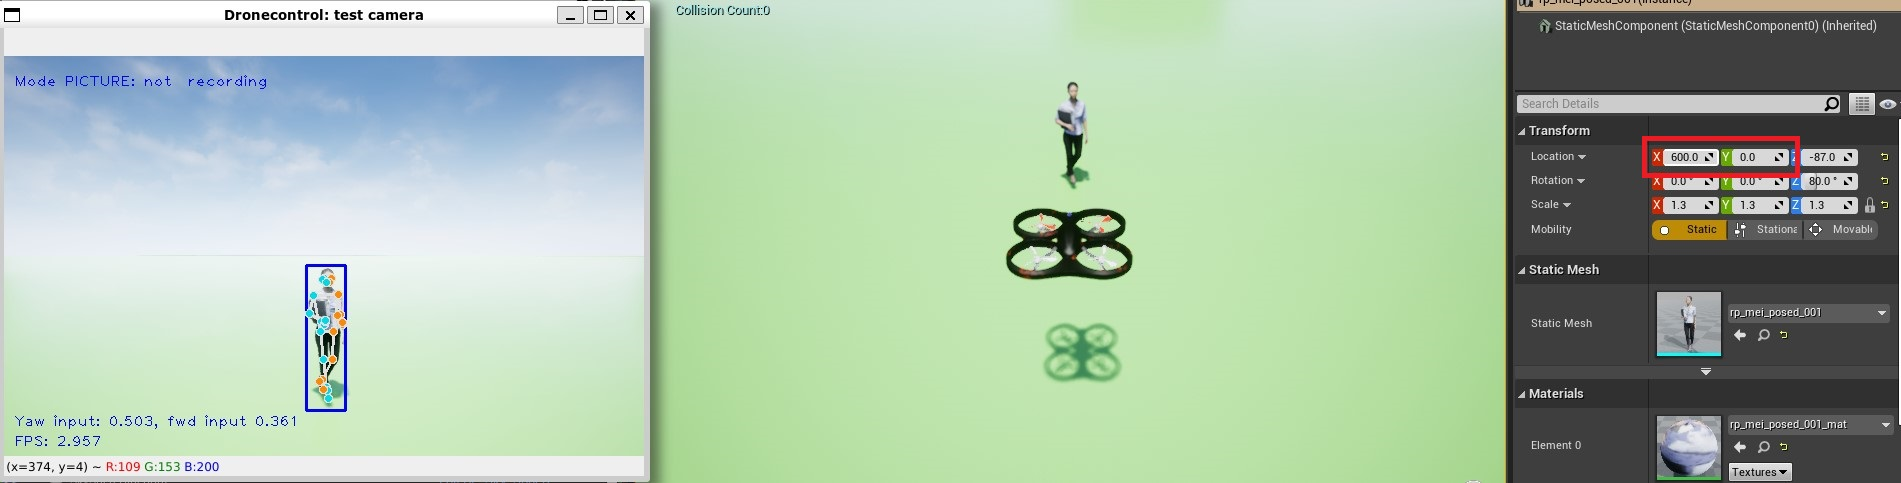
\includegraphics[width=\textwidth, keepaspectratio]{img/pid/tune-ref-pos.jpg}
  \caption{Reference position for the yaw and forward PID controllers. From left to right, the panels show the DroneVisionControl application window, the AirSim simulator world view and the world location of the human model in the simulator. The distance between the vehicle and the person is 600 units in the x direction and 0 units in the y direction.}
  \label{fig:tune-start-pos}
\end{figure}


\subsection{Yaw controller}
The first controller to tune will be the yaw controller. As mentioned, the first step is to select the sign of the process gain. In this case, the process variable or input to the controller is the normalized position of the detected person in the horizontal axis of the camera field of view, with 0 being the person situated on the left edge of the field of view and 1 on the right edge. A positive output on the controller produces a positive yaw velocity, which causes the vehicle to rotate towards the right. In response, the person moves to the left in the camera field of view, resulting in a decreasing input to the controller. Since positive outputs should cause increasing inputs, the sign of the output velocity needs to be inverted to avoid exponentially growing behaviour.

Once the sign is selected and before any parameters are tested, the starting position needs to be decided. In the starting position, the target person model is offset from the reference position shown in Figure \ref{fig:tune-start-pos} to provoke a step response in the controller. For the yaw controller, the offset will be 100 units in the y-axis. With the vehicle situated in the origin in the simulation environment, the person model should be situated at $x=500, y=100$. Figure \ref{fig:tune-ref-pos-yaw} shows the starting position in the simulation.

\begin{figure}[H]
  \centering
  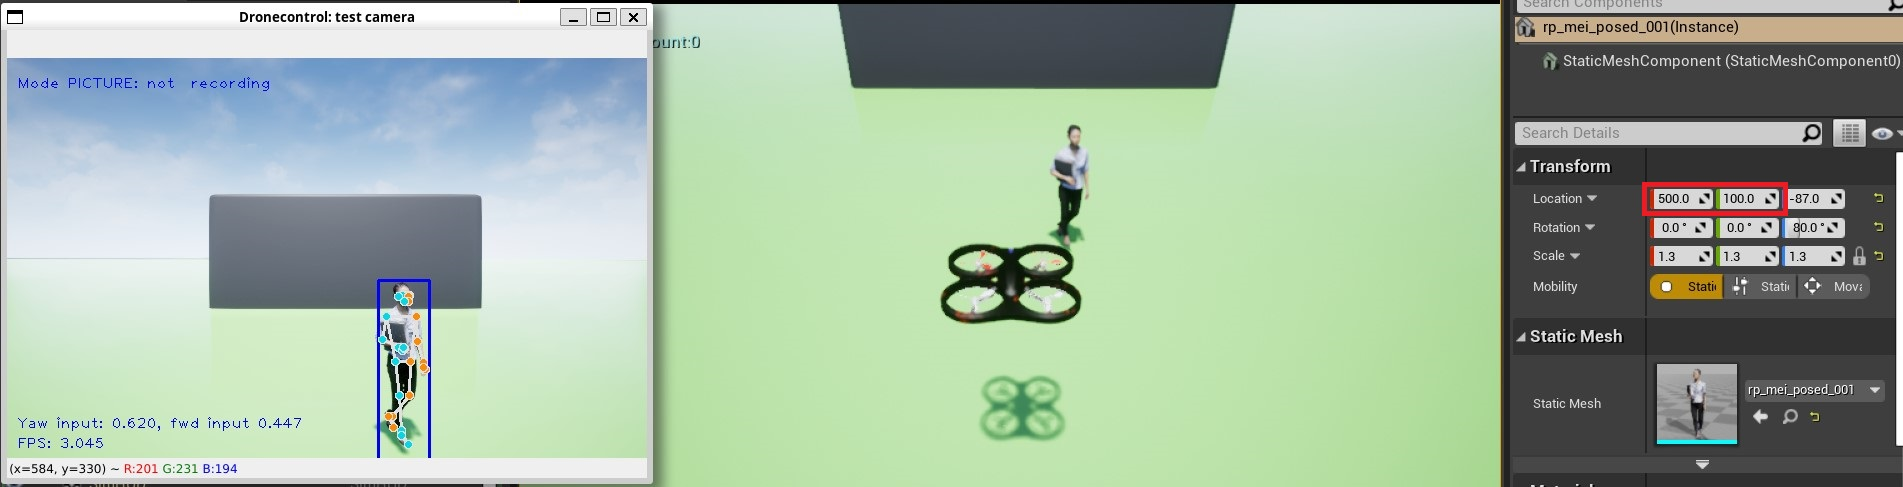
\includegraphics[width=\textwidth, keepaspectratio]{img/pid/tune-ref-pos-yaw.jpg}
  \caption{Starting position of the simulator for tuning the yaw controller. The human model is situated 500 units forward and 100 units to the right of the vehicle model.}
  \label{fig:tune-ref-pos-yaw}
\end{figure}

\subsubsection{Proportional component}

The proportional gain is the first parameter that needs to be tuned. The values chosen to test for $K_D$ range from 25 to 150 in steps of 25. To have a P-only controller during the test, the $K_I$ and $K_D$ components are set to 0. The results of the test are shown in Figure \ref{fig:tune-yaw-prop}.


\begin{figure}[H]
    \begin{minipage}[t]{0.5\linewidth}
        \centering
        \scalebox{0.55}{%% Creator: Matplotlib, PGF backend
%%
%% To include the figure in your LaTeX document, write
%%   \input{<filename>.pgf}
%%
%% Make sure the required packages are loaded in your preamble
%%   \usepackage{pgf}
%%
%% Also ensure that all the required font packages are loaded; for instance,
%% the lmodern package is sometimes necessary when using math font.
%%   \usepackage{lmodern}
%%
%% Figures using additional raster images can only be included by \input if
%% they are in the same directory as the main LaTeX file. For loading figures
%% from other directories you can use the `import` package
%%   \usepackage{import}
%%
%% and then include the figures with
%%   \import{<path to file>}{<filename>.pgf}
%%
%% Matplotlib used the following preamble
%%   \usepackage{fontspec}
%%   \setmainfont{DejaVuSerif.ttf}[Path=\detokenize{/home/lgonz/tfg-aero/tfg-giaa-dronecontrol/venv/lib/python3.8/site-packages/matplotlib/mpl-data/fonts/ttf/}]
%%   \setsansfont{DejaVuSans.ttf}[Path=\detokenize{/home/lgonz/tfg-aero/tfg-giaa-dronecontrol/venv/lib/python3.8/site-packages/matplotlib/mpl-data/fonts/ttf/}]
%%   \setmonofont{DejaVuSansMono.ttf}[Path=\detokenize{/home/lgonz/tfg-aero/tfg-giaa-dronecontrol/venv/lib/python3.8/site-packages/matplotlib/mpl-data/fonts/ttf/}]
%%
\begingroup%
\makeatletter%
\begin{pgfpicture}%
\pgfpathrectangle{\pgfpointorigin}{\pgfqpoint{6.400000in}{4.800000in}}%
\pgfusepath{use as bounding box, clip}%
\begin{pgfscope}%
\pgfsetbuttcap%
\pgfsetmiterjoin%
\definecolor{currentfill}{rgb}{1.000000,1.000000,1.000000}%
\pgfsetfillcolor{currentfill}%
\pgfsetlinewidth{0.000000pt}%
\definecolor{currentstroke}{rgb}{1.000000,1.000000,1.000000}%
\pgfsetstrokecolor{currentstroke}%
\pgfsetdash{}{0pt}%
\pgfpathmoveto{\pgfqpoint{0.000000in}{0.000000in}}%
\pgfpathlineto{\pgfqpoint{6.400000in}{0.000000in}}%
\pgfpathlineto{\pgfqpoint{6.400000in}{4.800000in}}%
\pgfpathlineto{\pgfqpoint{0.000000in}{4.800000in}}%
\pgfpathlineto{\pgfqpoint{0.000000in}{0.000000in}}%
\pgfpathclose%
\pgfusepath{fill}%
\end{pgfscope}%
\begin{pgfscope}%
\pgfsetbuttcap%
\pgfsetmiterjoin%
\definecolor{currentfill}{rgb}{1.000000,1.000000,1.000000}%
\pgfsetfillcolor{currentfill}%
\pgfsetlinewidth{0.000000pt}%
\definecolor{currentstroke}{rgb}{0.000000,0.000000,0.000000}%
\pgfsetstrokecolor{currentstroke}%
\pgfsetstrokeopacity{0.000000}%
\pgfsetdash{}{0pt}%
\pgfpathmoveto{\pgfqpoint{0.800000in}{0.528000in}}%
\pgfpathlineto{\pgfqpoint{5.760000in}{0.528000in}}%
\pgfpathlineto{\pgfqpoint{5.760000in}{4.224000in}}%
\pgfpathlineto{\pgfqpoint{0.800000in}{4.224000in}}%
\pgfpathlineto{\pgfqpoint{0.800000in}{0.528000in}}%
\pgfpathclose%
\pgfusepath{fill}%
\end{pgfscope}%
\begin{pgfscope}%
\pgfpathrectangle{\pgfqpoint{0.800000in}{0.528000in}}{\pgfqpoint{4.960000in}{3.696000in}}%
\pgfusepath{clip}%
\pgfsetrectcap%
\pgfsetroundjoin%
\pgfsetlinewidth{0.803000pt}%
\definecolor{currentstroke}{rgb}{0.690196,0.690196,0.690196}%
\pgfsetstrokecolor{currentstroke}%
\pgfsetdash{}{0pt}%
\pgfpathmoveto{\pgfqpoint{1.025455in}{0.528000in}}%
\pgfpathlineto{\pgfqpoint{1.025455in}{4.224000in}}%
\pgfusepath{stroke}%
\end{pgfscope}%
\begin{pgfscope}%
\pgfsetbuttcap%
\pgfsetroundjoin%
\definecolor{currentfill}{rgb}{0.000000,0.000000,0.000000}%
\pgfsetfillcolor{currentfill}%
\pgfsetlinewidth{0.803000pt}%
\definecolor{currentstroke}{rgb}{0.000000,0.000000,0.000000}%
\pgfsetstrokecolor{currentstroke}%
\pgfsetdash{}{0pt}%
\pgfsys@defobject{currentmarker}{\pgfqpoint{0.000000in}{-0.048611in}}{\pgfqpoint{0.000000in}{0.000000in}}{%
\pgfpathmoveto{\pgfqpoint{0.000000in}{0.000000in}}%
\pgfpathlineto{\pgfqpoint{0.000000in}{-0.048611in}}%
\pgfusepath{stroke,fill}%
}%
\begin{pgfscope}%
\pgfsys@transformshift{1.025455in}{0.528000in}%
\pgfsys@useobject{currentmarker}{}%
\end{pgfscope}%
\end{pgfscope}%
\begin{pgfscope}%
\definecolor{textcolor}{rgb}{0.000000,0.000000,0.000000}%
\pgfsetstrokecolor{textcolor}%
\pgfsetfillcolor{textcolor}%
\pgftext[x=1.025455in,y=0.430778in,,top]{\color{textcolor}\sffamily\fontsize{10.000000}{12.000000}\selectfont 0.0}%
\end{pgfscope}%
\begin{pgfscope}%
\pgfpathrectangle{\pgfqpoint{0.800000in}{0.528000in}}{\pgfqpoint{4.960000in}{3.696000in}}%
\pgfusepath{clip}%
\pgfsetrectcap%
\pgfsetroundjoin%
\pgfsetlinewidth{0.803000pt}%
\definecolor{currentstroke}{rgb}{0.690196,0.690196,0.690196}%
\pgfsetstrokecolor{currentstroke}%
\pgfsetdash{}{0pt}%
\pgfpathmoveto{\pgfqpoint{1.583185in}{0.528000in}}%
\pgfpathlineto{\pgfqpoint{1.583185in}{4.224000in}}%
\pgfusepath{stroke}%
\end{pgfscope}%
\begin{pgfscope}%
\pgfsetbuttcap%
\pgfsetroundjoin%
\definecolor{currentfill}{rgb}{0.000000,0.000000,0.000000}%
\pgfsetfillcolor{currentfill}%
\pgfsetlinewidth{0.803000pt}%
\definecolor{currentstroke}{rgb}{0.000000,0.000000,0.000000}%
\pgfsetstrokecolor{currentstroke}%
\pgfsetdash{}{0pt}%
\pgfsys@defobject{currentmarker}{\pgfqpoint{0.000000in}{-0.048611in}}{\pgfqpoint{0.000000in}{0.000000in}}{%
\pgfpathmoveto{\pgfqpoint{0.000000in}{0.000000in}}%
\pgfpathlineto{\pgfqpoint{0.000000in}{-0.048611in}}%
\pgfusepath{stroke,fill}%
}%
\begin{pgfscope}%
\pgfsys@transformshift{1.583185in}{0.528000in}%
\pgfsys@useobject{currentmarker}{}%
\end{pgfscope}%
\end{pgfscope}%
\begin{pgfscope}%
\definecolor{textcolor}{rgb}{0.000000,0.000000,0.000000}%
\pgfsetstrokecolor{textcolor}%
\pgfsetfillcolor{textcolor}%
\pgftext[x=1.583185in,y=0.430778in,,top]{\color{textcolor}\sffamily\fontsize{10.000000}{12.000000}\selectfont 2.5}%
\end{pgfscope}%
\begin{pgfscope}%
\pgfpathrectangle{\pgfqpoint{0.800000in}{0.528000in}}{\pgfqpoint{4.960000in}{3.696000in}}%
\pgfusepath{clip}%
\pgfsetrectcap%
\pgfsetroundjoin%
\pgfsetlinewidth{0.803000pt}%
\definecolor{currentstroke}{rgb}{0.690196,0.690196,0.690196}%
\pgfsetstrokecolor{currentstroke}%
\pgfsetdash{}{0pt}%
\pgfpathmoveto{\pgfqpoint{2.140916in}{0.528000in}}%
\pgfpathlineto{\pgfqpoint{2.140916in}{4.224000in}}%
\pgfusepath{stroke}%
\end{pgfscope}%
\begin{pgfscope}%
\pgfsetbuttcap%
\pgfsetroundjoin%
\definecolor{currentfill}{rgb}{0.000000,0.000000,0.000000}%
\pgfsetfillcolor{currentfill}%
\pgfsetlinewidth{0.803000pt}%
\definecolor{currentstroke}{rgb}{0.000000,0.000000,0.000000}%
\pgfsetstrokecolor{currentstroke}%
\pgfsetdash{}{0pt}%
\pgfsys@defobject{currentmarker}{\pgfqpoint{0.000000in}{-0.048611in}}{\pgfqpoint{0.000000in}{0.000000in}}{%
\pgfpathmoveto{\pgfqpoint{0.000000in}{0.000000in}}%
\pgfpathlineto{\pgfqpoint{0.000000in}{-0.048611in}}%
\pgfusepath{stroke,fill}%
}%
\begin{pgfscope}%
\pgfsys@transformshift{2.140916in}{0.528000in}%
\pgfsys@useobject{currentmarker}{}%
\end{pgfscope}%
\end{pgfscope}%
\begin{pgfscope}%
\definecolor{textcolor}{rgb}{0.000000,0.000000,0.000000}%
\pgfsetstrokecolor{textcolor}%
\pgfsetfillcolor{textcolor}%
\pgftext[x=2.140916in,y=0.430778in,,top]{\color{textcolor}\sffamily\fontsize{10.000000}{12.000000}\selectfont 5.0}%
\end{pgfscope}%
\begin{pgfscope}%
\pgfpathrectangle{\pgfqpoint{0.800000in}{0.528000in}}{\pgfqpoint{4.960000in}{3.696000in}}%
\pgfusepath{clip}%
\pgfsetrectcap%
\pgfsetroundjoin%
\pgfsetlinewidth{0.803000pt}%
\definecolor{currentstroke}{rgb}{0.690196,0.690196,0.690196}%
\pgfsetstrokecolor{currentstroke}%
\pgfsetdash{}{0pt}%
\pgfpathmoveto{\pgfqpoint{2.698647in}{0.528000in}}%
\pgfpathlineto{\pgfqpoint{2.698647in}{4.224000in}}%
\pgfusepath{stroke}%
\end{pgfscope}%
\begin{pgfscope}%
\pgfsetbuttcap%
\pgfsetroundjoin%
\definecolor{currentfill}{rgb}{0.000000,0.000000,0.000000}%
\pgfsetfillcolor{currentfill}%
\pgfsetlinewidth{0.803000pt}%
\definecolor{currentstroke}{rgb}{0.000000,0.000000,0.000000}%
\pgfsetstrokecolor{currentstroke}%
\pgfsetdash{}{0pt}%
\pgfsys@defobject{currentmarker}{\pgfqpoint{0.000000in}{-0.048611in}}{\pgfqpoint{0.000000in}{0.000000in}}{%
\pgfpathmoveto{\pgfqpoint{0.000000in}{0.000000in}}%
\pgfpathlineto{\pgfqpoint{0.000000in}{-0.048611in}}%
\pgfusepath{stroke,fill}%
}%
\begin{pgfscope}%
\pgfsys@transformshift{2.698647in}{0.528000in}%
\pgfsys@useobject{currentmarker}{}%
\end{pgfscope}%
\end{pgfscope}%
\begin{pgfscope}%
\definecolor{textcolor}{rgb}{0.000000,0.000000,0.000000}%
\pgfsetstrokecolor{textcolor}%
\pgfsetfillcolor{textcolor}%
\pgftext[x=2.698647in,y=0.430778in,,top]{\color{textcolor}\sffamily\fontsize{10.000000}{12.000000}\selectfont 7.5}%
\end{pgfscope}%
\begin{pgfscope}%
\pgfpathrectangle{\pgfqpoint{0.800000in}{0.528000in}}{\pgfqpoint{4.960000in}{3.696000in}}%
\pgfusepath{clip}%
\pgfsetrectcap%
\pgfsetroundjoin%
\pgfsetlinewidth{0.803000pt}%
\definecolor{currentstroke}{rgb}{0.690196,0.690196,0.690196}%
\pgfsetstrokecolor{currentstroke}%
\pgfsetdash{}{0pt}%
\pgfpathmoveto{\pgfqpoint{3.256378in}{0.528000in}}%
\pgfpathlineto{\pgfqpoint{3.256378in}{4.224000in}}%
\pgfusepath{stroke}%
\end{pgfscope}%
\begin{pgfscope}%
\pgfsetbuttcap%
\pgfsetroundjoin%
\definecolor{currentfill}{rgb}{0.000000,0.000000,0.000000}%
\pgfsetfillcolor{currentfill}%
\pgfsetlinewidth{0.803000pt}%
\definecolor{currentstroke}{rgb}{0.000000,0.000000,0.000000}%
\pgfsetstrokecolor{currentstroke}%
\pgfsetdash{}{0pt}%
\pgfsys@defobject{currentmarker}{\pgfqpoint{0.000000in}{-0.048611in}}{\pgfqpoint{0.000000in}{0.000000in}}{%
\pgfpathmoveto{\pgfqpoint{0.000000in}{0.000000in}}%
\pgfpathlineto{\pgfqpoint{0.000000in}{-0.048611in}}%
\pgfusepath{stroke,fill}%
}%
\begin{pgfscope}%
\pgfsys@transformshift{3.256378in}{0.528000in}%
\pgfsys@useobject{currentmarker}{}%
\end{pgfscope}%
\end{pgfscope}%
\begin{pgfscope}%
\definecolor{textcolor}{rgb}{0.000000,0.000000,0.000000}%
\pgfsetstrokecolor{textcolor}%
\pgfsetfillcolor{textcolor}%
\pgftext[x=3.256378in,y=0.430778in,,top]{\color{textcolor}\sffamily\fontsize{10.000000}{12.000000}\selectfont 10.0}%
\end{pgfscope}%
\begin{pgfscope}%
\pgfpathrectangle{\pgfqpoint{0.800000in}{0.528000in}}{\pgfqpoint{4.960000in}{3.696000in}}%
\pgfusepath{clip}%
\pgfsetrectcap%
\pgfsetroundjoin%
\pgfsetlinewidth{0.803000pt}%
\definecolor{currentstroke}{rgb}{0.690196,0.690196,0.690196}%
\pgfsetstrokecolor{currentstroke}%
\pgfsetdash{}{0pt}%
\pgfpathmoveto{\pgfqpoint{3.814109in}{0.528000in}}%
\pgfpathlineto{\pgfqpoint{3.814109in}{4.224000in}}%
\pgfusepath{stroke}%
\end{pgfscope}%
\begin{pgfscope}%
\pgfsetbuttcap%
\pgfsetroundjoin%
\definecolor{currentfill}{rgb}{0.000000,0.000000,0.000000}%
\pgfsetfillcolor{currentfill}%
\pgfsetlinewidth{0.803000pt}%
\definecolor{currentstroke}{rgb}{0.000000,0.000000,0.000000}%
\pgfsetstrokecolor{currentstroke}%
\pgfsetdash{}{0pt}%
\pgfsys@defobject{currentmarker}{\pgfqpoint{0.000000in}{-0.048611in}}{\pgfqpoint{0.000000in}{0.000000in}}{%
\pgfpathmoveto{\pgfqpoint{0.000000in}{0.000000in}}%
\pgfpathlineto{\pgfqpoint{0.000000in}{-0.048611in}}%
\pgfusepath{stroke,fill}%
}%
\begin{pgfscope}%
\pgfsys@transformshift{3.814109in}{0.528000in}%
\pgfsys@useobject{currentmarker}{}%
\end{pgfscope}%
\end{pgfscope}%
\begin{pgfscope}%
\definecolor{textcolor}{rgb}{0.000000,0.000000,0.000000}%
\pgfsetstrokecolor{textcolor}%
\pgfsetfillcolor{textcolor}%
\pgftext[x=3.814109in,y=0.430778in,,top]{\color{textcolor}\sffamily\fontsize{10.000000}{12.000000}\selectfont 12.5}%
\end{pgfscope}%
\begin{pgfscope}%
\pgfpathrectangle{\pgfqpoint{0.800000in}{0.528000in}}{\pgfqpoint{4.960000in}{3.696000in}}%
\pgfusepath{clip}%
\pgfsetrectcap%
\pgfsetroundjoin%
\pgfsetlinewidth{0.803000pt}%
\definecolor{currentstroke}{rgb}{0.690196,0.690196,0.690196}%
\pgfsetstrokecolor{currentstroke}%
\pgfsetdash{}{0pt}%
\pgfpathmoveto{\pgfqpoint{4.371840in}{0.528000in}}%
\pgfpathlineto{\pgfqpoint{4.371840in}{4.224000in}}%
\pgfusepath{stroke}%
\end{pgfscope}%
\begin{pgfscope}%
\pgfsetbuttcap%
\pgfsetroundjoin%
\definecolor{currentfill}{rgb}{0.000000,0.000000,0.000000}%
\pgfsetfillcolor{currentfill}%
\pgfsetlinewidth{0.803000pt}%
\definecolor{currentstroke}{rgb}{0.000000,0.000000,0.000000}%
\pgfsetstrokecolor{currentstroke}%
\pgfsetdash{}{0pt}%
\pgfsys@defobject{currentmarker}{\pgfqpoint{0.000000in}{-0.048611in}}{\pgfqpoint{0.000000in}{0.000000in}}{%
\pgfpathmoveto{\pgfqpoint{0.000000in}{0.000000in}}%
\pgfpathlineto{\pgfqpoint{0.000000in}{-0.048611in}}%
\pgfusepath{stroke,fill}%
}%
\begin{pgfscope}%
\pgfsys@transformshift{4.371840in}{0.528000in}%
\pgfsys@useobject{currentmarker}{}%
\end{pgfscope}%
\end{pgfscope}%
\begin{pgfscope}%
\definecolor{textcolor}{rgb}{0.000000,0.000000,0.000000}%
\pgfsetstrokecolor{textcolor}%
\pgfsetfillcolor{textcolor}%
\pgftext[x=4.371840in,y=0.430778in,,top]{\color{textcolor}\sffamily\fontsize{10.000000}{12.000000}\selectfont 15.0}%
\end{pgfscope}%
\begin{pgfscope}%
\pgfpathrectangle{\pgfqpoint{0.800000in}{0.528000in}}{\pgfqpoint{4.960000in}{3.696000in}}%
\pgfusepath{clip}%
\pgfsetrectcap%
\pgfsetroundjoin%
\pgfsetlinewidth{0.803000pt}%
\definecolor{currentstroke}{rgb}{0.690196,0.690196,0.690196}%
\pgfsetstrokecolor{currentstroke}%
\pgfsetdash{}{0pt}%
\pgfpathmoveto{\pgfqpoint{4.929570in}{0.528000in}}%
\pgfpathlineto{\pgfqpoint{4.929570in}{4.224000in}}%
\pgfusepath{stroke}%
\end{pgfscope}%
\begin{pgfscope}%
\pgfsetbuttcap%
\pgfsetroundjoin%
\definecolor{currentfill}{rgb}{0.000000,0.000000,0.000000}%
\pgfsetfillcolor{currentfill}%
\pgfsetlinewidth{0.803000pt}%
\definecolor{currentstroke}{rgb}{0.000000,0.000000,0.000000}%
\pgfsetstrokecolor{currentstroke}%
\pgfsetdash{}{0pt}%
\pgfsys@defobject{currentmarker}{\pgfqpoint{0.000000in}{-0.048611in}}{\pgfqpoint{0.000000in}{0.000000in}}{%
\pgfpathmoveto{\pgfqpoint{0.000000in}{0.000000in}}%
\pgfpathlineto{\pgfqpoint{0.000000in}{-0.048611in}}%
\pgfusepath{stroke,fill}%
}%
\begin{pgfscope}%
\pgfsys@transformshift{4.929570in}{0.528000in}%
\pgfsys@useobject{currentmarker}{}%
\end{pgfscope}%
\end{pgfscope}%
\begin{pgfscope}%
\definecolor{textcolor}{rgb}{0.000000,0.000000,0.000000}%
\pgfsetstrokecolor{textcolor}%
\pgfsetfillcolor{textcolor}%
\pgftext[x=4.929570in,y=0.430778in,,top]{\color{textcolor}\sffamily\fontsize{10.000000}{12.000000}\selectfont 17.5}%
\end{pgfscope}%
\begin{pgfscope}%
\pgfpathrectangle{\pgfqpoint{0.800000in}{0.528000in}}{\pgfqpoint{4.960000in}{3.696000in}}%
\pgfusepath{clip}%
\pgfsetrectcap%
\pgfsetroundjoin%
\pgfsetlinewidth{0.803000pt}%
\definecolor{currentstroke}{rgb}{0.690196,0.690196,0.690196}%
\pgfsetstrokecolor{currentstroke}%
\pgfsetdash{}{0pt}%
\pgfpathmoveto{\pgfqpoint{5.487301in}{0.528000in}}%
\pgfpathlineto{\pgfqpoint{5.487301in}{4.224000in}}%
\pgfusepath{stroke}%
\end{pgfscope}%
\begin{pgfscope}%
\pgfsetbuttcap%
\pgfsetroundjoin%
\definecolor{currentfill}{rgb}{0.000000,0.000000,0.000000}%
\pgfsetfillcolor{currentfill}%
\pgfsetlinewidth{0.803000pt}%
\definecolor{currentstroke}{rgb}{0.000000,0.000000,0.000000}%
\pgfsetstrokecolor{currentstroke}%
\pgfsetdash{}{0pt}%
\pgfsys@defobject{currentmarker}{\pgfqpoint{0.000000in}{-0.048611in}}{\pgfqpoint{0.000000in}{0.000000in}}{%
\pgfpathmoveto{\pgfqpoint{0.000000in}{0.000000in}}%
\pgfpathlineto{\pgfqpoint{0.000000in}{-0.048611in}}%
\pgfusepath{stroke,fill}%
}%
\begin{pgfscope}%
\pgfsys@transformshift{5.487301in}{0.528000in}%
\pgfsys@useobject{currentmarker}{}%
\end{pgfscope}%
\end{pgfscope}%
\begin{pgfscope}%
\definecolor{textcolor}{rgb}{0.000000,0.000000,0.000000}%
\pgfsetstrokecolor{textcolor}%
\pgfsetfillcolor{textcolor}%
\pgftext[x=5.487301in,y=0.430778in,,top]{\color{textcolor}\sffamily\fontsize{10.000000}{12.000000}\selectfont 20.0}%
\end{pgfscope}%
\begin{pgfscope}%
\definecolor{textcolor}{rgb}{0.000000,0.000000,0.000000}%
\pgfsetstrokecolor{textcolor}%
\pgfsetfillcolor{textcolor}%
\pgftext[x=3.280000in,y=0.240809in,,top]{\color{textcolor}\sffamily\fontsize{10.000000}{12.000000}\selectfont time [s]}%
\end{pgfscope}%
\begin{pgfscope}%
\pgfpathrectangle{\pgfqpoint{0.800000in}{0.528000in}}{\pgfqpoint{4.960000in}{3.696000in}}%
\pgfusepath{clip}%
\pgfsetrectcap%
\pgfsetroundjoin%
\pgfsetlinewidth{0.803000pt}%
\definecolor{currentstroke}{rgb}{0.690196,0.690196,0.690196}%
\pgfsetstrokecolor{currentstroke}%
\pgfsetdash{}{0pt}%
\pgfpathmoveto{\pgfqpoint{0.800000in}{0.569608in}}%
\pgfpathlineto{\pgfqpoint{5.760000in}{0.569608in}}%
\pgfusepath{stroke}%
\end{pgfscope}%
\begin{pgfscope}%
\pgfsetbuttcap%
\pgfsetroundjoin%
\definecolor{currentfill}{rgb}{0.000000,0.000000,0.000000}%
\pgfsetfillcolor{currentfill}%
\pgfsetlinewidth{0.803000pt}%
\definecolor{currentstroke}{rgb}{0.000000,0.000000,0.000000}%
\pgfsetstrokecolor{currentstroke}%
\pgfsetdash{}{0pt}%
\pgfsys@defobject{currentmarker}{\pgfqpoint{-0.048611in}{0.000000in}}{\pgfqpoint{-0.000000in}{0.000000in}}{%
\pgfpathmoveto{\pgfqpoint{-0.000000in}{0.000000in}}%
\pgfpathlineto{\pgfqpoint{-0.048611in}{0.000000in}}%
\pgfusepath{stroke,fill}%
}%
\begin{pgfscope}%
\pgfsys@transformshift{0.800000in}{0.569608in}%
\pgfsys@useobject{currentmarker}{}%
\end{pgfscope}%
\end{pgfscope}%
\begin{pgfscope}%
\definecolor{textcolor}{rgb}{0.000000,0.000000,0.000000}%
\pgfsetstrokecolor{textcolor}%
\pgfsetfillcolor{textcolor}%
\pgftext[x=0.285508in, y=0.516846in, left, base]{\color{textcolor}\sffamily\fontsize{10.000000}{12.000000}\selectfont \ensuremath{-}0.12}%
\end{pgfscope}%
\begin{pgfscope}%
\pgfpathrectangle{\pgfqpoint{0.800000in}{0.528000in}}{\pgfqpoint{4.960000in}{3.696000in}}%
\pgfusepath{clip}%
\pgfsetrectcap%
\pgfsetroundjoin%
\pgfsetlinewidth{0.803000pt}%
\definecolor{currentstroke}{rgb}{0.690196,0.690196,0.690196}%
\pgfsetstrokecolor{currentstroke}%
\pgfsetdash{}{0pt}%
\pgfpathmoveto{\pgfqpoint{0.800000in}{1.085253in}}%
\pgfpathlineto{\pgfqpoint{5.760000in}{1.085253in}}%
\pgfusepath{stroke}%
\end{pgfscope}%
\begin{pgfscope}%
\pgfsetbuttcap%
\pgfsetroundjoin%
\definecolor{currentfill}{rgb}{0.000000,0.000000,0.000000}%
\pgfsetfillcolor{currentfill}%
\pgfsetlinewidth{0.803000pt}%
\definecolor{currentstroke}{rgb}{0.000000,0.000000,0.000000}%
\pgfsetstrokecolor{currentstroke}%
\pgfsetdash{}{0pt}%
\pgfsys@defobject{currentmarker}{\pgfqpoint{-0.048611in}{0.000000in}}{\pgfqpoint{-0.000000in}{0.000000in}}{%
\pgfpathmoveto{\pgfqpoint{-0.000000in}{0.000000in}}%
\pgfpathlineto{\pgfqpoint{-0.048611in}{0.000000in}}%
\pgfusepath{stroke,fill}%
}%
\begin{pgfscope}%
\pgfsys@transformshift{0.800000in}{1.085253in}%
\pgfsys@useobject{currentmarker}{}%
\end{pgfscope}%
\end{pgfscope}%
\begin{pgfscope}%
\definecolor{textcolor}{rgb}{0.000000,0.000000,0.000000}%
\pgfsetstrokecolor{textcolor}%
\pgfsetfillcolor{textcolor}%
\pgftext[x=0.285508in, y=1.032491in, left, base]{\color{textcolor}\sffamily\fontsize{10.000000}{12.000000}\selectfont \ensuremath{-}0.10}%
\end{pgfscope}%
\begin{pgfscope}%
\pgfpathrectangle{\pgfqpoint{0.800000in}{0.528000in}}{\pgfqpoint{4.960000in}{3.696000in}}%
\pgfusepath{clip}%
\pgfsetrectcap%
\pgfsetroundjoin%
\pgfsetlinewidth{0.803000pt}%
\definecolor{currentstroke}{rgb}{0.690196,0.690196,0.690196}%
\pgfsetstrokecolor{currentstroke}%
\pgfsetdash{}{0pt}%
\pgfpathmoveto{\pgfqpoint{0.800000in}{1.600897in}}%
\pgfpathlineto{\pgfqpoint{5.760000in}{1.600897in}}%
\pgfusepath{stroke}%
\end{pgfscope}%
\begin{pgfscope}%
\pgfsetbuttcap%
\pgfsetroundjoin%
\definecolor{currentfill}{rgb}{0.000000,0.000000,0.000000}%
\pgfsetfillcolor{currentfill}%
\pgfsetlinewidth{0.803000pt}%
\definecolor{currentstroke}{rgb}{0.000000,0.000000,0.000000}%
\pgfsetstrokecolor{currentstroke}%
\pgfsetdash{}{0pt}%
\pgfsys@defobject{currentmarker}{\pgfqpoint{-0.048611in}{0.000000in}}{\pgfqpoint{-0.000000in}{0.000000in}}{%
\pgfpathmoveto{\pgfqpoint{-0.000000in}{0.000000in}}%
\pgfpathlineto{\pgfqpoint{-0.048611in}{0.000000in}}%
\pgfusepath{stroke,fill}%
}%
\begin{pgfscope}%
\pgfsys@transformshift{0.800000in}{1.600897in}%
\pgfsys@useobject{currentmarker}{}%
\end{pgfscope}%
\end{pgfscope}%
\begin{pgfscope}%
\definecolor{textcolor}{rgb}{0.000000,0.000000,0.000000}%
\pgfsetstrokecolor{textcolor}%
\pgfsetfillcolor{textcolor}%
\pgftext[x=0.285508in, y=1.548136in, left, base]{\color{textcolor}\sffamily\fontsize{10.000000}{12.000000}\selectfont \ensuremath{-}0.08}%
\end{pgfscope}%
\begin{pgfscope}%
\pgfpathrectangle{\pgfqpoint{0.800000in}{0.528000in}}{\pgfqpoint{4.960000in}{3.696000in}}%
\pgfusepath{clip}%
\pgfsetrectcap%
\pgfsetroundjoin%
\pgfsetlinewidth{0.803000pt}%
\definecolor{currentstroke}{rgb}{0.690196,0.690196,0.690196}%
\pgfsetstrokecolor{currentstroke}%
\pgfsetdash{}{0pt}%
\pgfpathmoveto{\pgfqpoint{0.800000in}{2.116542in}}%
\pgfpathlineto{\pgfqpoint{5.760000in}{2.116542in}}%
\pgfusepath{stroke}%
\end{pgfscope}%
\begin{pgfscope}%
\pgfsetbuttcap%
\pgfsetroundjoin%
\definecolor{currentfill}{rgb}{0.000000,0.000000,0.000000}%
\pgfsetfillcolor{currentfill}%
\pgfsetlinewidth{0.803000pt}%
\definecolor{currentstroke}{rgb}{0.000000,0.000000,0.000000}%
\pgfsetstrokecolor{currentstroke}%
\pgfsetdash{}{0pt}%
\pgfsys@defobject{currentmarker}{\pgfqpoint{-0.048611in}{0.000000in}}{\pgfqpoint{-0.000000in}{0.000000in}}{%
\pgfpathmoveto{\pgfqpoint{-0.000000in}{0.000000in}}%
\pgfpathlineto{\pgfqpoint{-0.048611in}{0.000000in}}%
\pgfusepath{stroke,fill}%
}%
\begin{pgfscope}%
\pgfsys@transformshift{0.800000in}{2.116542in}%
\pgfsys@useobject{currentmarker}{}%
\end{pgfscope}%
\end{pgfscope}%
\begin{pgfscope}%
\definecolor{textcolor}{rgb}{0.000000,0.000000,0.000000}%
\pgfsetstrokecolor{textcolor}%
\pgfsetfillcolor{textcolor}%
\pgftext[x=0.285508in, y=2.063781in, left, base]{\color{textcolor}\sffamily\fontsize{10.000000}{12.000000}\selectfont \ensuremath{-}0.06}%
\end{pgfscope}%
\begin{pgfscope}%
\pgfpathrectangle{\pgfqpoint{0.800000in}{0.528000in}}{\pgfqpoint{4.960000in}{3.696000in}}%
\pgfusepath{clip}%
\pgfsetrectcap%
\pgfsetroundjoin%
\pgfsetlinewidth{0.803000pt}%
\definecolor{currentstroke}{rgb}{0.690196,0.690196,0.690196}%
\pgfsetstrokecolor{currentstroke}%
\pgfsetdash{}{0pt}%
\pgfpathmoveto{\pgfqpoint{0.800000in}{2.632187in}}%
\pgfpathlineto{\pgfqpoint{5.760000in}{2.632187in}}%
\pgfusepath{stroke}%
\end{pgfscope}%
\begin{pgfscope}%
\pgfsetbuttcap%
\pgfsetroundjoin%
\definecolor{currentfill}{rgb}{0.000000,0.000000,0.000000}%
\pgfsetfillcolor{currentfill}%
\pgfsetlinewidth{0.803000pt}%
\definecolor{currentstroke}{rgb}{0.000000,0.000000,0.000000}%
\pgfsetstrokecolor{currentstroke}%
\pgfsetdash{}{0pt}%
\pgfsys@defobject{currentmarker}{\pgfqpoint{-0.048611in}{0.000000in}}{\pgfqpoint{-0.000000in}{0.000000in}}{%
\pgfpathmoveto{\pgfqpoint{-0.000000in}{0.000000in}}%
\pgfpathlineto{\pgfqpoint{-0.048611in}{0.000000in}}%
\pgfusepath{stroke,fill}%
}%
\begin{pgfscope}%
\pgfsys@transformshift{0.800000in}{2.632187in}%
\pgfsys@useobject{currentmarker}{}%
\end{pgfscope}%
\end{pgfscope}%
\begin{pgfscope}%
\definecolor{textcolor}{rgb}{0.000000,0.000000,0.000000}%
\pgfsetstrokecolor{textcolor}%
\pgfsetfillcolor{textcolor}%
\pgftext[x=0.285508in, y=2.579426in, left, base]{\color{textcolor}\sffamily\fontsize{10.000000}{12.000000}\selectfont \ensuremath{-}0.04}%
\end{pgfscope}%
\begin{pgfscope}%
\pgfpathrectangle{\pgfqpoint{0.800000in}{0.528000in}}{\pgfqpoint{4.960000in}{3.696000in}}%
\pgfusepath{clip}%
\pgfsetrectcap%
\pgfsetroundjoin%
\pgfsetlinewidth{0.803000pt}%
\definecolor{currentstroke}{rgb}{0.690196,0.690196,0.690196}%
\pgfsetstrokecolor{currentstroke}%
\pgfsetdash{}{0pt}%
\pgfpathmoveto{\pgfqpoint{0.800000in}{3.147832in}}%
\pgfpathlineto{\pgfqpoint{5.760000in}{3.147832in}}%
\pgfusepath{stroke}%
\end{pgfscope}%
\begin{pgfscope}%
\pgfsetbuttcap%
\pgfsetroundjoin%
\definecolor{currentfill}{rgb}{0.000000,0.000000,0.000000}%
\pgfsetfillcolor{currentfill}%
\pgfsetlinewidth{0.803000pt}%
\definecolor{currentstroke}{rgb}{0.000000,0.000000,0.000000}%
\pgfsetstrokecolor{currentstroke}%
\pgfsetdash{}{0pt}%
\pgfsys@defobject{currentmarker}{\pgfqpoint{-0.048611in}{0.000000in}}{\pgfqpoint{-0.000000in}{0.000000in}}{%
\pgfpathmoveto{\pgfqpoint{-0.000000in}{0.000000in}}%
\pgfpathlineto{\pgfqpoint{-0.048611in}{0.000000in}}%
\pgfusepath{stroke,fill}%
}%
\begin{pgfscope}%
\pgfsys@transformshift{0.800000in}{3.147832in}%
\pgfsys@useobject{currentmarker}{}%
\end{pgfscope}%
\end{pgfscope}%
\begin{pgfscope}%
\definecolor{textcolor}{rgb}{0.000000,0.000000,0.000000}%
\pgfsetstrokecolor{textcolor}%
\pgfsetfillcolor{textcolor}%
\pgftext[x=0.285508in, y=3.095070in, left, base]{\color{textcolor}\sffamily\fontsize{10.000000}{12.000000}\selectfont \ensuremath{-}0.02}%
\end{pgfscope}%
\begin{pgfscope}%
\pgfpathrectangle{\pgfqpoint{0.800000in}{0.528000in}}{\pgfqpoint{4.960000in}{3.696000in}}%
\pgfusepath{clip}%
\pgfsetrectcap%
\pgfsetroundjoin%
\pgfsetlinewidth{0.803000pt}%
\definecolor{currentstroke}{rgb}{0.690196,0.690196,0.690196}%
\pgfsetstrokecolor{currentstroke}%
\pgfsetdash{}{0pt}%
\pgfpathmoveto{\pgfqpoint{0.800000in}{3.663477in}}%
\pgfpathlineto{\pgfqpoint{5.760000in}{3.663477in}}%
\pgfusepath{stroke}%
\end{pgfscope}%
\begin{pgfscope}%
\pgfsetbuttcap%
\pgfsetroundjoin%
\definecolor{currentfill}{rgb}{0.000000,0.000000,0.000000}%
\pgfsetfillcolor{currentfill}%
\pgfsetlinewidth{0.803000pt}%
\definecolor{currentstroke}{rgb}{0.000000,0.000000,0.000000}%
\pgfsetstrokecolor{currentstroke}%
\pgfsetdash{}{0pt}%
\pgfsys@defobject{currentmarker}{\pgfqpoint{-0.048611in}{0.000000in}}{\pgfqpoint{-0.000000in}{0.000000in}}{%
\pgfpathmoveto{\pgfqpoint{-0.000000in}{0.000000in}}%
\pgfpathlineto{\pgfqpoint{-0.048611in}{0.000000in}}%
\pgfusepath{stroke,fill}%
}%
\begin{pgfscope}%
\pgfsys@transformshift{0.800000in}{3.663477in}%
\pgfsys@useobject{currentmarker}{}%
\end{pgfscope}%
\end{pgfscope}%
\begin{pgfscope}%
\definecolor{textcolor}{rgb}{0.000000,0.000000,0.000000}%
\pgfsetstrokecolor{textcolor}%
\pgfsetfillcolor{textcolor}%
\pgftext[x=0.393533in, y=3.610715in, left, base]{\color{textcolor}\sffamily\fontsize{10.000000}{12.000000}\selectfont 0.00}%
\end{pgfscope}%
\begin{pgfscope}%
\pgfpathrectangle{\pgfqpoint{0.800000in}{0.528000in}}{\pgfqpoint{4.960000in}{3.696000in}}%
\pgfusepath{clip}%
\pgfsetrectcap%
\pgfsetroundjoin%
\pgfsetlinewidth{0.803000pt}%
\definecolor{currentstroke}{rgb}{0.690196,0.690196,0.690196}%
\pgfsetstrokecolor{currentstroke}%
\pgfsetdash{}{0pt}%
\pgfpathmoveto{\pgfqpoint{0.800000in}{4.179122in}}%
\pgfpathlineto{\pgfqpoint{5.760000in}{4.179122in}}%
\pgfusepath{stroke}%
\end{pgfscope}%
\begin{pgfscope}%
\pgfsetbuttcap%
\pgfsetroundjoin%
\definecolor{currentfill}{rgb}{0.000000,0.000000,0.000000}%
\pgfsetfillcolor{currentfill}%
\pgfsetlinewidth{0.803000pt}%
\definecolor{currentstroke}{rgb}{0.000000,0.000000,0.000000}%
\pgfsetstrokecolor{currentstroke}%
\pgfsetdash{}{0pt}%
\pgfsys@defobject{currentmarker}{\pgfqpoint{-0.048611in}{0.000000in}}{\pgfqpoint{-0.000000in}{0.000000in}}{%
\pgfpathmoveto{\pgfqpoint{-0.000000in}{0.000000in}}%
\pgfpathlineto{\pgfqpoint{-0.048611in}{0.000000in}}%
\pgfusepath{stroke,fill}%
}%
\begin{pgfscope}%
\pgfsys@transformshift{0.800000in}{4.179122in}%
\pgfsys@useobject{currentmarker}{}%
\end{pgfscope}%
\end{pgfscope}%
\begin{pgfscope}%
\definecolor{textcolor}{rgb}{0.000000,0.000000,0.000000}%
\pgfsetstrokecolor{textcolor}%
\pgfsetfillcolor{textcolor}%
\pgftext[x=0.393533in, y=4.126360in, left, base]{\color{textcolor}\sffamily\fontsize{10.000000}{12.000000}\selectfont 0.02}%
\end{pgfscope}%
\begin{pgfscope}%
\definecolor{textcolor}{rgb}{0.000000,0.000000,0.000000}%
\pgfsetstrokecolor{textcolor}%
\pgfsetfillcolor{textcolor}%
\pgftext[x=0.229952in,y=2.376000in,,bottom,rotate=90.000000]{\color{textcolor}\sffamily\fontsize{10.000000}{12.000000}\selectfont Computed error [-]}%
\end{pgfscope}%
\begin{pgfscope}%
\pgfpathrectangle{\pgfqpoint{0.800000in}{0.528000in}}{\pgfqpoint{4.960000in}{3.696000in}}%
\pgfusepath{clip}%
\pgfsetrectcap%
\pgfsetroundjoin%
\pgfsetlinewidth{1.505625pt}%
\definecolor{currentstroke}{rgb}{0.121569,0.466667,0.705882}%
\pgfsetstrokecolor{currentstroke}%
\pgfsetdash{}{0pt}%
\pgfpathmoveto{\pgfqpoint{1.025455in}{0.712081in}}%
\pgfpathlineto{\pgfqpoint{1.063776in}{0.696000in}}%
\pgfpathlineto{\pgfqpoint{1.138623in}{0.711314in}}%
\pgfpathlineto{\pgfqpoint{1.212806in}{0.842489in}}%
\pgfpathlineto{\pgfqpoint{1.286280in}{1.145714in}}%
\pgfpathlineto{\pgfqpoint{1.360571in}{1.432675in}}%
\pgfpathlineto{\pgfqpoint{1.434952in}{1.732022in}}%
\pgfpathlineto{\pgfqpoint{1.508998in}{1.885539in}}%
\pgfpathlineto{\pgfqpoint{1.584714in}{2.026093in}}%
\pgfpathlineto{\pgfqpoint{1.661929in}{2.188805in}}%
\pgfpathlineto{\pgfqpoint{1.735143in}{2.398230in}}%
\pgfpathlineto{\pgfqpoint{1.808687in}{2.513056in}}%
\pgfpathlineto{\pgfqpoint{1.882936in}{2.615015in}}%
\pgfpathlineto{\pgfqpoint{1.957436in}{2.722138in}}%
\pgfpathlineto{\pgfqpoint{2.032221in}{2.777356in}}%
\pgfpathlineto{\pgfqpoint{2.106580in}{2.859100in}}%
\pgfpathlineto{\pgfqpoint{2.181303in}{2.942273in}}%
\pgfpathlineto{\pgfqpoint{2.255350in}{2.980329in}}%
\pgfpathlineto{\pgfqpoint{2.330461in}{3.026141in}}%
\pgfpathlineto{\pgfqpoint{2.404739in}{3.104836in}}%
\pgfpathlineto{\pgfqpoint{2.479219in}{3.127947in}}%
\pgfpathlineto{\pgfqpoint{2.555322in}{3.157530in}}%
\pgfpathlineto{\pgfqpoint{2.629577in}{3.191829in}}%
\pgfpathlineto{\pgfqpoint{2.703086in}{3.226892in}}%
\pgfpathlineto{\pgfqpoint{2.777270in}{3.264032in}}%
\pgfpathlineto{\pgfqpoint{2.852756in}{3.305920in}}%
\pgfpathlineto{\pgfqpoint{2.927602in}{3.347435in}}%
\pgfpathlineto{\pgfqpoint{3.001582in}{3.470657in}}%
\pgfpathlineto{\pgfqpoint{3.076834in}{3.439839in}}%
\pgfpathlineto{\pgfqpoint{3.150951in}{3.438114in}}%
\pgfpathlineto{\pgfqpoint{3.227261in}{3.451766in}}%
\pgfpathlineto{\pgfqpoint{3.301360in}{3.527610in}}%
\pgfpathlineto{\pgfqpoint{3.375878in}{3.537456in}}%
\pgfpathlineto{\pgfqpoint{3.452246in}{3.572963in}}%
\pgfpathlineto{\pgfqpoint{3.527990in}{3.568798in}}%
\pgfpathlineto{\pgfqpoint{3.599038in}{3.585830in}}%
\pgfpathlineto{\pgfqpoint{3.673314in}{3.600962in}}%
\pgfpathlineto{\pgfqpoint{3.747844in}{3.582396in}}%
\pgfpathlineto{\pgfqpoint{3.822123in}{3.621213in}}%
\pgfpathlineto{\pgfqpoint{3.896442in}{3.633919in}}%
\pgfpathlineto{\pgfqpoint{3.970902in}{3.650584in}}%
\pgfpathlineto{\pgfqpoint{4.045637in}{3.655765in}}%
\pgfpathlineto{\pgfqpoint{4.119856in}{3.655431in}}%
\pgfpathlineto{\pgfqpoint{4.193845in}{3.653380in}}%
\pgfpathlineto{\pgfqpoint{4.268656in}{3.626673in}}%
\pgfpathlineto{\pgfqpoint{4.345033in}{3.667087in}}%
\pgfpathlineto{\pgfqpoint{4.418046in}{3.665640in}}%
\pgfpathlineto{\pgfqpoint{4.492418in}{3.666472in}}%
\pgfpathlineto{\pgfqpoint{4.566377in}{3.692297in}}%
\pgfpathlineto{\pgfqpoint{4.640637in}{3.686526in}}%
\pgfpathlineto{\pgfqpoint{4.715036in}{3.681462in}}%
\pgfpathlineto{\pgfqpoint{4.789632in}{3.685527in}}%
\pgfpathlineto{\pgfqpoint{4.864110in}{3.690495in}}%
\pgfpathlineto{\pgfqpoint{4.938524in}{3.745055in}}%
\pgfpathlineto{\pgfqpoint{5.012461in}{3.724862in}}%
\pgfpathlineto{\pgfqpoint{5.086863in}{3.709051in}}%
\pgfpathlineto{\pgfqpoint{5.161604in}{3.740338in}}%
\pgfpathlineto{\pgfqpoint{5.237893in}{3.668447in}}%
\pgfpathlineto{\pgfqpoint{5.311107in}{3.632056in}}%
\pgfpathlineto{\pgfqpoint{5.386056in}{3.632079in}}%
\pgfpathlineto{\pgfqpoint{5.459939in}{3.762462in}}%
\pgfpathlineto{\pgfqpoint{5.534545in}{3.729021in}}%
\pgfusepath{stroke}%
\end{pgfscope}%
\begin{pgfscope}%
\pgfpathrectangle{\pgfqpoint{0.800000in}{0.528000in}}{\pgfqpoint{4.960000in}{3.696000in}}%
\pgfusepath{clip}%
\pgfsetrectcap%
\pgfsetroundjoin%
\pgfsetlinewidth{1.505625pt}%
\definecolor{currentstroke}{rgb}{1.000000,0.498039,0.054902}%
\pgfsetstrokecolor{currentstroke}%
\pgfsetdash{}{0pt}%
\pgfpathmoveto{\pgfqpoint{1.025455in}{0.750514in}}%
\pgfpathlineto{\pgfqpoint{1.099065in}{0.757257in}}%
\pgfpathlineto{\pgfqpoint{1.172846in}{0.987325in}}%
\pgfpathlineto{\pgfqpoint{1.246645in}{1.344846in}}%
\pgfpathlineto{\pgfqpoint{1.322501in}{1.874728in}}%
\pgfpathlineto{\pgfqpoint{1.396760in}{2.239682in}}%
\pgfpathlineto{\pgfqpoint{1.473513in}{2.589436in}}%
\pgfpathlineto{\pgfqpoint{1.546544in}{2.872297in}}%
\pgfpathlineto{\pgfqpoint{1.621097in}{3.148842in}}%
\pgfpathlineto{\pgfqpoint{1.696748in}{3.316592in}}%
\pgfpathlineto{\pgfqpoint{1.771019in}{3.388146in}}%
\pgfpathlineto{\pgfqpoint{1.848364in}{3.447828in}}%
\pgfpathlineto{\pgfqpoint{1.920266in}{3.485764in}}%
\pgfpathlineto{\pgfqpoint{1.994195in}{3.507296in}}%
\pgfpathlineto{\pgfqpoint{2.068179in}{3.527716in}}%
\pgfpathlineto{\pgfqpoint{2.142269in}{3.506451in}}%
\pgfpathlineto{\pgfqpoint{2.216486in}{3.530340in}}%
\pgfpathlineto{\pgfqpoint{2.291371in}{3.555824in}}%
\pgfpathlineto{\pgfqpoint{2.365491in}{3.553536in}}%
\pgfpathlineto{\pgfqpoint{2.439982in}{3.579730in}}%
\pgfpathlineto{\pgfqpoint{2.514002in}{3.554164in}}%
\pgfpathlineto{\pgfqpoint{2.589901in}{3.554021in}}%
\pgfpathlineto{\pgfqpoint{2.663464in}{3.563023in}}%
\pgfpathlineto{\pgfqpoint{2.737949in}{3.573612in}}%
\pgfpathlineto{\pgfqpoint{2.812354in}{3.609140in}}%
\pgfpathlineto{\pgfqpoint{2.886469in}{3.616459in}}%
\pgfpathlineto{\pgfqpoint{2.960992in}{3.633508in}}%
\pgfpathlineto{\pgfqpoint{3.035396in}{3.652534in}}%
\pgfpathlineto{\pgfqpoint{3.109941in}{3.674541in}}%
\pgfpathlineto{\pgfqpoint{3.185940in}{3.687335in}}%
\pgfpathlineto{\pgfqpoint{3.258333in}{3.691343in}}%
\pgfpathlineto{\pgfqpoint{3.334870in}{3.691110in}}%
\pgfpathlineto{\pgfqpoint{3.409005in}{3.687159in}}%
\pgfpathlineto{\pgfqpoint{3.483374in}{3.683740in}}%
\pgfpathlineto{\pgfqpoint{3.557709in}{3.680826in}}%
\pgfpathlineto{\pgfqpoint{3.635481in}{3.675678in}}%
\pgfpathlineto{\pgfqpoint{3.706173in}{3.679590in}}%
\pgfpathlineto{\pgfqpoint{3.780753in}{3.680221in}}%
\pgfpathlineto{\pgfqpoint{3.855154in}{3.680541in}}%
\pgfpathlineto{\pgfqpoint{3.929719in}{3.668267in}}%
\pgfpathlineto{\pgfqpoint{4.003795in}{3.680027in}}%
\pgfpathlineto{\pgfqpoint{4.078260in}{3.697320in}}%
\pgfpathlineto{\pgfqpoint{4.152395in}{3.627613in}}%
\pgfpathlineto{\pgfqpoint{4.228322in}{3.611994in}}%
\pgfpathlineto{\pgfqpoint{4.302367in}{3.614911in}}%
\pgfpathlineto{\pgfqpoint{4.375819in}{3.659697in}}%
\pgfpathlineto{\pgfqpoint{4.451286in}{3.652071in}}%
\pgfpathlineto{\pgfqpoint{4.525804in}{3.639211in}}%
\pgfpathlineto{\pgfqpoint{4.600850in}{3.638705in}}%
\pgfpathlineto{\pgfqpoint{4.675521in}{3.642074in}}%
\pgfpathlineto{\pgfqpoint{4.752222in}{3.646738in}}%
\pgfpathlineto{\pgfqpoint{4.828037in}{3.659036in}}%
\pgfpathlineto{\pgfqpoint{4.902395in}{3.669353in}}%
\pgfpathlineto{\pgfqpoint{4.976465in}{3.735929in}}%
\pgfpathlineto{\pgfqpoint{5.051645in}{3.730041in}}%
\pgfpathlineto{\pgfqpoint{5.125255in}{3.670775in}}%
\pgfpathlineto{\pgfqpoint{5.199740in}{3.584650in}}%
\pgfpathlineto{\pgfqpoint{5.273953in}{3.551455in}}%
\pgfpathlineto{\pgfqpoint{5.348063in}{3.551045in}}%
\pgfpathlineto{\pgfqpoint{5.422504in}{3.690645in}}%
\pgfpathlineto{\pgfqpoint{5.497107in}{3.645863in}}%
\pgfusepath{stroke}%
\end{pgfscope}%
\begin{pgfscope}%
\pgfpathrectangle{\pgfqpoint{0.800000in}{0.528000in}}{\pgfqpoint{4.960000in}{3.696000in}}%
\pgfusepath{clip}%
\pgfsetrectcap%
\pgfsetroundjoin%
\pgfsetlinewidth{1.505625pt}%
\definecolor{currentstroke}{rgb}{0.172549,0.627451,0.172549}%
\pgfsetstrokecolor{currentstroke}%
\pgfsetdash{}{0pt}%
\pgfpathmoveto{\pgfqpoint{1.025455in}{0.765793in}}%
\pgfpathlineto{\pgfqpoint{1.099911in}{0.778590in}}%
\pgfpathlineto{\pgfqpoint{1.175324in}{1.101696in}}%
\pgfpathlineto{\pgfqpoint{1.250759in}{1.485395in}}%
\pgfpathlineto{\pgfqpoint{1.324208in}{1.960597in}}%
\pgfpathlineto{\pgfqpoint{1.398758in}{2.483777in}}%
\pgfpathlineto{\pgfqpoint{1.473239in}{2.891969in}}%
\pgfpathlineto{\pgfqpoint{1.547019in}{3.273010in}}%
\pgfpathlineto{\pgfqpoint{1.621688in}{3.570346in}}%
\pgfpathlineto{\pgfqpoint{1.695783in}{3.737484in}}%
\pgfpathlineto{\pgfqpoint{1.770461in}{3.723029in}}%
\pgfpathlineto{\pgfqpoint{1.847841in}{3.758239in}}%
\pgfpathlineto{\pgfqpoint{1.918992in}{3.806586in}}%
\pgfpathlineto{\pgfqpoint{1.995729in}{3.754568in}}%
\pgfpathlineto{\pgfqpoint{2.071400in}{3.692826in}}%
\pgfpathlineto{\pgfqpoint{2.144749in}{3.643533in}}%
\pgfpathlineto{\pgfqpoint{2.218626in}{3.614652in}}%
\pgfpathlineto{\pgfqpoint{2.293223in}{3.637023in}}%
\pgfpathlineto{\pgfqpoint{2.367600in}{3.571304in}}%
\pgfpathlineto{\pgfqpoint{2.441953in}{3.675501in}}%
\pgfpathlineto{\pgfqpoint{2.516471in}{3.635010in}}%
\pgfpathlineto{\pgfqpoint{2.590935in}{3.634243in}}%
\pgfpathlineto{\pgfqpoint{2.665483in}{3.625403in}}%
\pgfpathlineto{\pgfqpoint{2.739264in}{3.615084in}}%
\pgfpathlineto{\pgfqpoint{2.814189in}{3.605215in}}%
\pgfpathlineto{\pgfqpoint{2.889825in}{3.622084in}}%
\pgfpathlineto{\pgfqpoint{2.963704in}{3.622582in}}%
\pgfpathlineto{\pgfqpoint{3.037334in}{3.622381in}}%
\pgfpathlineto{\pgfqpoint{3.112176in}{3.616297in}}%
\pgfpathlineto{\pgfqpoint{3.186516in}{3.611273in}}%
\pgfpathlineto{\pgfqpoint{3.260694in}{3.617859in}}%
\pgfpathlineto{\pgfqpoint{3.335034in}{3.668712in}}%
\pgfpathlineto{\pgfqpoint{3.409356in}{3.666525in}}%
\pgfpathlineto{\pgfqpoint{3.484633in}{3.658872in}}%
\pgfpathlineto{\pgfqpoint{3.558101in}{3.645881in}}%
\pgfpathlineto{\pgfqpoint{3.632383in}{3.643402in}}%
\pgfpathlineto{\pgfqpoint{3.707011in}{3.718062in}}%
\pgfpathlineto{\pgfqpoint{3.783326in}{3.724008in}}%
\pgfpathlineto{\pgfqpoint{3.856908in}{3.651340in}}%
\pgfpathlineto{\pgfqpoint{3.930715in}{3.624424in}}%
\pgfpathlineto{\pgfqpoint{4.004643in}{3.608829in}}%
\pgfpathlineto{\pgfqpoint{4.078590in}{3.604696in}}%
\pgfpathlineto{\pgfqpoint{4.154100in}{3.598036in}}%
\pgfpathlineto{\pgfqpoint{4.228692in}{3.617646in}}%
\pgfpathlineto{\pgfqpoint{4.302687in}{3.635894in}}%
\pgfpathlineto{\pgfqpoint{4.377390in}{3.639674in}}%
\pgfpathlineto{\pgfqpoint{4.451459in}{3.645503in}}%
\pgfpathlineto{\pgfqpoint{4.525943in}{3.653420in}}%
\pgfpathlineto{\pgfqpoint{4.601122in}{3.653522in}}%
\pgfpathlineto{\pgfqpoint{4.675193in}{3.655071in}}%
\pgfpathlineto{\pgfqpoint{4.750877in}{3.645047in}}%
\pgfpathlineto{\pgfqpoint{4.824357in}{3.650157in}}%
\pgfpathlineto{\pgfqpoint{4.898213in}{3.650645in}}%
\pgfpathlineto{\pgfqpoint{4.972646in}{3.598496in}}%
\pgfpathlineto{\pgfqpoint{5.047668in}{3.594487in}}%
\pgfpathlineto{\pgfqpoint{5.121956in}{3.607148in}}%
\pgfpathlineto{\pgfqpoint{5.196176in}{3.684920in}}%
\pgfpathlineto{\pgfqpoint{5.270506in}{3.672852in}}%
\pgfpathlineto{\pgfqpoint{5.345043in}{3.654725in}}%
\pgfpathlineto{\pgfqpoint{5.419263in}{3.645731in}}%
\pgfpathlineto{\pgfqpoint{5.493699in}{3.679618in}}%
\pgfusepath{stroke}%
\end{pgfscope}%
\begin{pgfscope}%
\pgfpathrectangle{\pgfqpoint{0.800000in}{0.528000in}}{\pgfqpoint{4.960000in}{3.696000in}}%
\pgfusepath{clip}%
\pgfsetrectcap%
\pgfsetroundjoin%
\pgfsetlinewidth{1.505625pt}%
\definecolor{currentstroke}{rgb}{0.839216,0.152941,0.156863}%
\pgfsetstrokecolor{currentstroke}%
\pgfsetdash{}{0pt}%
\pgfpathmoveto{\pgfqpoint{1.025455in}{0.764512in}}%
\pgfpathlineto{\pgfqpoint{1.099317in}{0.769619in}}%
\pgfpathlineto{\pgfqpoint{1.173519in}{1.044913in}}%
\pgfpathlineto{\pgfqpoint{1.247511in}{1.400453in}}%
\pgfpathlineto{\pgfqpoint{1.322201in}{1.894242in}}%
\pgfpathlineto{\pgfqpoint{1.396396in}{2.435620in}}%
\pgfpathlineto{\pgfqpoint{1.470917in}{2.917505in}}%
\pgfpathlineto{\pgfqpoint{1.545546in}{3.273112in}}%
\pgfpathlineto{\pgfqpoint{1.619703in}{3.789598in}}%
\pgfpathlineto{\pgfqpoint{1.694012in}{3.825462in}}%
\pgfpathlineto{\pgfqpoint{1.768885in}{3.975413in}}%
\pgfpathlineto{\pgfqpoint{1.842986in}{3.891544in}}%
\pgfpathlineto{\pgfqpoint{1.919062in}{3.808414in}}%
\pgfpathlineto{\pgfqpoint{1.992356in}{3.719060in}}%
\pgfpathlineto{\pgfqpoint{2.066206in}{3.630064in}}%
\pgfpathlineto{\pgfqpoint{2.140388in}{3.547560in}}%
\pgfpathlineto{\pgfqpoint{2.214802in}{3.524054in}}%
\pgfpathlineto{\pgfqpoint{2.288995in}{3.553333in}}%
\pgfpathlineto{\pgfqpoint{2.363309in}{3.578748in}}%
\pgfpathlineto{\pgfqpoint{2.437570in}{3.591594in}}%
\pgfpathlineto{\pgfqpoint{2.512228in}{3.616208in}}%
\pgfpathlineto{\pgfqpoint{2.586632in}{3.628265in}}%
\pgfpathlineto{\pgfqpoint{2.661688in}{3.657657in}}%
\pgfpathlineto{\pgfqpoint{2.735747in}{3.734210in}}%
\pgfpathlineto{\pgfqpoint{2.809657in}{3.729330in}}%
\pgfpathlineto{\pgfqpoint{2.883897in}{3.693667in}}%
\pgfpathlineto{\pgfqpoint{2.958353in}{3.680043in}}%
\pgfpathlineto{\pgfqpoint{3.032628in}{3.624015in}}%
\pgfpathlineto{\pgfqpoint{3.107069in}{3.627603in}}%
\pgfpathlineto{\pgfqpoint{3.181518in}{3.608076in}}%
\pgfpathlineto{\pgfqpoint{3.255803in}{3.598243in}}%
\pgfpathlineto{\pgfqpoint{3.330082in}{3.588613in}}%
\pgfpathlineto{\pgfqpoint{3.406248in}{3.582035in}}%
\pgfpathlineto{\pgfqpoint{3.482771in}{3.576513in}}%
\pgfpathlineto{\pgfqpoint{3.555301in}{3.596836in}}%
\pgfpathlineto{\pgfqpoint{3.629360in}{3.617336in}}%
\pgfpathlineto{\pgfqpoint{3.703565in}{3.636909in}}%
\pgfpathlineto{\pgfqpoint{3.778024in}{3.639804in}}%
\pgfpathlineto{\pgfqpoint{3.852388in}{3.675679in}}%
\pgfpathlineto{\pgfqpoint{3.927125in}{3.686831in}}%
\pgfpathlineto{\pgfqpoint{4.002276in}{3.697293in}}%
\pgfpathlineto{\pgfqpoint{4.076613in}{3.693312in}}%
\pgfpathlineto{\pgfqpoint{4.150560in}{3.687977in}}%
\pgfpathlineto{\pgfqpoint{4.225595in}{3.666941in}}%
\pgfpathlineto{\pgfqpoint{4.302408in}{3.683137in}}%
\pgfpathlineto{\pgfqpoint{4.375572in}{3.652386in}}%
\pgfpathlineto{\pgfqpoint{4.449438in}{3.748699in}}%
\pgfpathlineto{\pgfqpoint{4.523700in}{3.679239in}}%
\pgfpathlineto{\pgfqpoint{4.598169in}{3.617208in}}%
\pgfpathlineto{\pgfqpoint{4.672232in}{3.571684in}}%
\pgfpathlineto{\pgfqpoint{4.747518in}{3.575020in}}%
\pgfpathlineto{\pgfqpoint{4.822072in}{3.543237in}}%
\pgfpathlineto{\pgfqpoint{4.897366in}{3.539970in}}%
\pgfpathlineto{\pgfqpoint{4.971408in}{3.546933in}}%
\pgfpathlineto{\pgfqpoint{5.045575in}{3.583280in}}%
\pgfpathlineto{\pgfqpoint{5.120129in}{3.595381in}}%
\pgfpathlineto{\pgfqpoint{5.197079in}{3.614207in}}%
\pgfpathlineto{\pgfqpoint{5.270598in}{3.679506in}}%
\pgfpathlineto{\pgfqpoint{5.345079in}{3.697385in}}%
\pgfpathlineto{\pgfqpoint{5.419659in}{3.709422in}}%
\pgfpathlineto{\pgfqpoint{5.493677in}{3.706048in}}%
\pgfusepath{stroke}%
\end{pgfscope}%
\begin{pgfscope}%
\pgfpathrectangle{\pgfqpoint{0.800000in}{0.528000in}}{\pgfqpoint{4.960000in}{3.696000in}}%
\pgfusepath{clip}%
\pgfsetrectcap%
\pgfsetroundjoin%
\pgfsetlinewidth{1.505625pt}%
\definecolor{currentstroke}{rgb}{0.580392,0.403922,0.741176}%
\pgfsetstrokecolor{currentstroke}%
\pgfsetdash{}{0pt}%
\pgfpathmoveto{\pgfqpoint{1.025455in}{0.738618in}}%
\pgfpathlineto{\pgfqpoint{1.100458in}{0.792579in}}%
\pgfpathlineto{\pgfqpoint{1.176281in}{1.035238in}}%
\pgfpathlineto{\pgfqpoint{1.250820in}{1.480665in}}%
\pgfpathlineto{\pgfqpoint{1.324749in}{1.935529in}}%
\pgfpathlineto{\pgfqpoint{1.398416in}{2.435732in}}%
\pgfpathlineto{\pgfqpoint{1.472778in}{2.927914in}}%
\pgfpathlineto{\pgfqpoint{1.547787in}{3.331854in}}%
\pgfpathlineto{\pgfqpoint{1.622083in}{3.708665in}}%
\pgfpathlineto{\pgfqpoint{1.696655in}{3.964779in}}%
\pgfpathlineto{\pgfqpoint{1.771695in}{4.012352in}}%
\pgfpathlineto{\pgfqpoint{1.846473in}{4.056000in}}%
\pgfpathlineto{\pgfqpoint{1.921333in}{3.800301in}}%
\pgfpathlineto{\pgfqpoint{1.997868in}{3.684595in}}%
\pgfpathlineto{\pgfqpoint{2.071678in}{3.590967in}}%
\pgfpathlineto{\pgfqpoint{2.145699in}{3.519844in}}%
\pgfpathlineto{\pgfqpoint{2.220025in}{3.464517in}}%
\pgfpathlineto{\pgfqpoint{2.294077in}{3.457185in}}%
\pgfpathlineto{\pgfqpoint{2.370747in}{3.504670in}}%
\pgfpathlineto{\pgfqpoint{2.443124in}{3.580497in}}%
\pgfpathlineto{\pgfqpoint{2.517862in}{3.582568in}}%
\pgfpathlineto{\pgfqpoint{2.591929in}{3.630165in}}%
\pgfpathlineto{\pgfqpoint{2.666223in}{3.673735in}}%
\pgfpathlineto{\pgfqpoint{2.740918in}{3.773446in}}%
\pgfpathlineto{\pgfqpoint{2.816862in}{3.865754in}}%
\pgfpathlineto{\pgfqpoint{2.890082in}{3.816657in}}%
\pgfpathlineto{\pgfqpoint{2.964029in}{3.739903in}}%
\pgfpathlineto{\pgfqpoint{3.038293in}{3.644611in}}%
\pgfpathlineto{\pgfqpoint{3.112766in}{3.639869in}}%
\pgfpathlineto{\pgfqpoint{3.186957in}{3.542315in}}%
\pgfpathlineto{\pgfqpoint{3.261805in}{3.535236in}}%
\pgfpathlineto{\pgfqpoint{3.337022in}{3.530606in}}%
\pgfpathlineto{\pgfqpoint{3.411398in}{3.528227in}}%
\pgfpathlineto{\pgfqpoint{3.486552in}{3.557848in}}%
\pgfpathlineto{\pgfqpoint{3.560422in}{3.569954in}}%
\pgfpathlineto{\pgfqpoint{3.634412in}{3.681334in}}%
\pgfpathlineto{\pgfqpoint{3.710497in}{3.696935in}}%
\pgfpathlineto{\pgfqpoint{3.783965in}{3.722865in}}%
\pgfpathlineto{\pgfqpoint{3.857775in}{3.721750in}}%
\pgfpathlineto{\pgfqpoint{3.931643in}{3.719083in}}%
\pgfpathlineto{\pgfqpoint{4.006370in}{3.711775in}}%
\pgfpathlineto{\pgfqpoint{4.080629in}{3.711661in}}%
\pgfpathlineto{\pgfqpoint{4.155515in}{3.714135in}}%
\pgfpathlineto{\pgfqpoint{4.229449in}{3.615028in}}%
\pgfpathlineto{\pgfqpoint{4.304294in}{3.531718in}}%
\pgfpathlineto{\pgfqpoint{4.378164in}{3.534218in}}%
\pgfpathlineto{\pgfqpoint{4.454060in}{3.567497in}}%
\pgfpathlineto{\pgfqpoint{4.528649in}{3.587800in}}%
\pgfpathlineto{\pgfqpoint{4.605303in}{3.593102in}}%
\pgfpathlineto{\pgfqpoint{4.678615in}{3.627127in}}%
\pgfpathlineto{\pgfqpoint{4.752839in}{3.671951in}}%
\pgfpathlineto{\pgfqpoint{4.827129in}{3.717907in}}%
\pgfpathlineto{\pgfqpoint{4.902033in}{3.737871in}}%
\pgfpathlineto{\pgfqpoint{4.977876in}{3.868177in}}%
\pgfpathlineto{\pgfqpoint{5.051683in}{3.825276in}}%
\pgfpathlineto{\pgfqpoint{5.125830in}{3.746545in}}%
\pgfpathlineto{\pgfqpoint{5.200384in}{3.706173in}}%
\pgfpathlineto{\pgfqpoint{5.274235in}{3.608876in}}%
\pgfpathlineto{\pgfqpoint{5.348695in}{3.518185in}}%
\pgfpathlineto{\pgfqpoint{5.423195in}{3.532442in}}%
\pgfpathlineto{\pgfqpoint{5.499079in}{3.530912in}}%
\pgfusepath{stroke}%
\end{pgfscope}%
\begin{pgfscope}%
\pgfpathrectangle{\pgfqpoint{0.800000in}{0.528000in}}{\pgfqpoint{4.960000in}{3.696000in}}%
\pgfusepath{clip}%
\pgfsetrectcap%
\pgfsetroundjoin%
\pgfsetlinewidth{1.505625pt}%
\definecolor{currentstroke}{rgb}{0.549020,0.337255,0.294118}%
\pgfsetstrokecolor{currentstroke}%
\pgfsetdash{}{0pt}%
\pgfpathmoveto{\pgfqpoint{1.025455in}{0.742256in}}%
\pgfpathlineto{\pgfqpoint{1.099647in}{0.778325in}}%
\pgfpathlineto{\pgfqpoint{1.174084in}{1.100498in}}%
\pgfpathlineto{\pgfqpoint{1.248390in}{1.493512in}}%
\pgfpathlineto{\pgfqpoint{1.322841in}{2.017005in}}%
\pgfpathlineto{\pgfqpoint{1.397621in}{2.506135in}}%
\pgfpathlineto{\pgfqpoint{1.472134in}{2.916922in}}%
\pgfpathlineto{\pgfqpoint{1.546661in}{3.490019in}}%
\pgfpathlineto{\pgfqpoint{1.622031in}{3.799356in}}%
\pgfpathlineto{\pgfqpoint{1.696124in}{3.997648in}}%
\pgfpathlineto{\pgfqpoint{1.770359in}{3.988773in}}%
\pgfpathlineto{\pgfqpoint{1.844945in}{3.952996in}}%
\pgfpathlineto{\pgfqpoint{1.919056in}{3.788517in}}%
\pgfpathlineto{\pgfqpoint{1.993644in}{3.591868in}}%
\pgfpathlineto{\pgfqpoint{2.067688in}{3.459063in}}%
\pgfpathlineto{\pgfqpoint{2.142953in}{3.408651in}}%
\pgfpathlineto{\pgfqpoint{2.216798in}{3.441772in}}%
\pgfpathlineto{\pgfqpoint{2.290796in}{3.469168in}}%
\pgfpathlineto{\pgfqpoint{2.365613in}{3.532840in}}%
\pgfpathlineto{\pgfqpoint{2.442489in}{3.641766in}}%
\pgfpathlineto{\pgfqpoint{2.515846in}{3.745393in}}%
\pgfpathlineto{\pgfqpoint{2.589371in}{3.804057in}}%
\pgfpathlineto{\pgfqpoint{2.663477in}{3.789106in}}%
\pgfpathlineto{\pgfqpoint{2.738336in}{3.806464in}}%
\pgfpathlineto{\pgfqpoint{2.812747in}{3.757123in}}%
\pgfpathlineto{\pgfqpoint{2.887592in}{3.751660in}}%
\pgfpathlineto{\pgfqpoint{2.961704in}{3.673283in}}%
\pgfpathlineto{\pgfqpoint{3.036167in}{3.619228in}}%
\pgfpathlineto{\pgfqpoint{3.109768in}{3.530612in}}%
\pgfpathlineto{\pgfqpoint{3.184331in}{3.533370in}}%
\pgfpathlineto{\pgfqpoint{3.258978in}{3.545157in}}%
\pgfpathlineto{\pgfqpoint{3.335761in}{3.602010in}}%
\pgfpathlineto{\pgfqpoint{3.410308in}{3.651377in}}%
\pgfpathlineto{\pgfqpoint{3.483913in}{3.693571in}}%
\pgfpathlineto{\pgfqpoint{3.558745in}{3.735727in}}%
\pgfpathlineto{\pgfqpoint{3.633531in}{3.747311in}}%
\pgfpathlineto{\pgfqpoint{3.708051in}{3.751267in}}%
\pgfpathlineto{\pgfqpoint{3.782670in}{3.742350in}}%
\pgfpathlineto{\pgfqpoint{3.856790in}{3.690299in}}%
\pgfpathlineto{\pgfqpoint{3.931143in}{3.634825in}}%
\pgfpathlineto{\pgfqpoint{4.005704in}{3.562697in}}%
\pgfpathlineto{\pgfqpoint{4.080418in}{3.544429in}}%
\pgfpathlineto{\pgfqpoint{4.155350in}{3.582879in}}%
\pgfpathlineto{\pgfqpoint{4.232876in}{3.599450in}}%
\pgfpathlineto{\pgfqpoint{4.305808in}{3.653715in}}%
\pgfpathlineto{\pgfqpoint{4.379205in}{3.671428in}}%
\pgfpathlineto{\pgfqpoint{4.453262in}{3.677173in}}%
\pgfpathlineto{\pgfqpoint{4.528297in}{3.687170in}}%
\pgfpathlineto{\pgfqpoint{4.603125in}{3.706063in}}%
\pgfpathlineto{\pgfqpoint{4.677816in}{3.717514in}}%
\pgfpathlineto{\pgfqpoint{4.751560in}{3.702962in}}%
\pgfpathlineto{\pgfqpoint{4.826891in}{3.685078in}}%
\pgfpathlineto{\pgfqpoint{4.901387in}{3.671163in}}%
\pgfpathlineto{\pgfqpoint{4.975726in}{3.643229in}}%
\pgfpathlineto{\pgfqpoint{5.050456in}{3.633133in}}%
\pgfpathlineto{\pgfqpoint{5.124767in}{3.628443in}}%
\pgfpathlineto{\pgfqpoint{5.199653in}{3.628585in}}%
\pgfpathlineto{\pgfqpoint{5.274321in}{3.696190in}}%
\pgfpathlineto{\pgfqpoint{5.349479in}{3.707169in}}%
\pgfpathlineto{\pgfqpoint{5.424210in}{3.748363in}}%
\pgfpathlineto{\pgfqpoint{5.499007in}{3.724123in}}%
\pgfusepath{stroke}%
\end{pgfscope}%
\begin{pgfscope}%
\pgfsetrectcap%
\pgfsetmiterjoin%
\pgfsetlinewidth{0.803000pt}%
\definecolor{currentstroke}{rgb}{0.000000,0.000000,0.000000}%
\pgfsetstrokecolor{currentstroke}%
\pgfsetdash{}{0pt}%
\pgfpathmoveto{\pgfqpoint{0.800000in}{0.528000in}}%
\pgfpathlineto{\pgfqpoint{0.800000in}{4.224000in}}%
\pgfusepath{stroke}%
\end{pgfscope}%
\begin{pgfscope}%
\pgfsetrectcap%
\pgfsetmiterjoin%
\pgfsetlinewidth{0.803000pt}%
\definecolor{currentstroke}{rgb}{0.000000,0.000000,0.000000}%
\pgfsetstrokecolor{currentstroke}%
\pgfsetdash{}{0pt}%
\pgfpathmoveto{\pgfqpoint{5.760000in}{0.528000in}}%
\pgfpathlineto{\pgfqpoint{5.760000in}{4.224000in}}%
\pgfusepath{stroke}%
\end{pgfscope}%
\begin{pgfscope}%
\pgfsetrectcap%
\pgfsetmiterjoin%
\pgfsetlinewidth{0.803000pt}%
\definecolor{currentstroke}{rgb}{0.000000,0.000000,0.000000}%
\pgfsetstrokecolor{currentstroke}%
\pgfsetdash{}{0pt}%
\pgfpathmoveto{\pgfqpoint{0.800000in}{0.528000in}}%
\pgfpathlineto{\pgfqpoint{5.760000in}{0.528000in}}%
\pgfusepath{stroke}%
\end{pgfscope}%
\begin{pgfscope}%
\pgfsetrectcap%
\pgfsetmiterjoin%
\pgfsetlinewidth{0.803000pt}%
\definecolor{currentstroke}{rgb}{0.000000,0.000000,0.000000}%
\pgfsetstrokecolor{currentstroke}%
\pgfsetdash{}{0pt}%
\pgfpathmoveto{\pgfqpoint{0.800000in}{4.224000in}}%
\pgfpathlineto{\pgfqpoint{5.760000in}{4.224000in}}%
\pgfusepath{stroke}%
\end{pgfscope}%
\begin{pgfscope}%
\definecolor{textcolor}{rgb}{0.000000,0.000000,0.000000}%
\pgfsetstrokecolor{textcolor}%
\pgfsetfillcolor{textcolor}%
\pgftext[x=3.280000in,y=4.307333in,,base]{\color{textcolor}\sffamily\fontsize{12.000000}{14.400000}\selectfont Yaw controller input}%
\end{pgfscope}%
\begin{pgfscope}%
\pgfsetbuttcap%
\pgfsetmiterjoin%
\definecolor{currentfill}{rgb}{1.000000,1.000000,1.000000}%
\pgfsetfillcolor{currentfill}%
\pgfsetfillopacity{0.800000}%
\pgfsetlinewidth{1.003750pt}%
\definecolor{currentstroke}{rgb}{0.800000,0.800000,0.800000}%
\pgfsetstrokecolor{currentstroke}%
\pgfsetstrokeopacity{0.800000}%
\pgfsetdash{}{0pt}%
\pgfpathmoveto{\pgfqpoint{4.953237in}{0.597444in}}%
\pgfpathlineto{\pgfqpoint{5.662778in}{0.597444in}}%
\pgfpathquadraticcurveto{\pgfqpoint{5.690556in}{0.597444in}}{\pgfqpoint{5.690556in}{0.625222in}}%
\pgfpathlineto{\pgfqpoint{5.690556in}{1.834477in}}%
\pgfpathquadraticcurveto{\pgfqpoint{5.690556in}{1.862254in}}{\pgfqpoint{5.662778in}{1.862254in}}%
\pgfpathlineto{\pgfqpoint{4.953237in}{1.862254in}}%
\pgfpathquadraticcurveto{\pgfqpoint{4.925460in}{1.862254in}}{\pgfqpoint{4.925460in}{1.834477in}}%
\pgfpathlineto{\pgfqpoint{4.925460in}{0.625222in}}%
\pgfpathquadraticcurveto{\pgfqpoint{4.925460in}{0.597444in}}{\pgfqpoint{4.953237in}{0.597444in}}%
\pgfpathlineto{\pgfqpoint{4.953237in}{0.597444in}}%
\pgfpathclose%
\pgfusepath{stroke,fill}%
\end{pgfscope}%
\begin{pgfscope}%
\pgfsetrectcap%
\pgfsetroundjoin%
\pgfsetlinewidth{1.505625pt}%
\definecolor{currentstroke}{rgb}{0.121569,0.466667,0.705882}%
\pgfsetstrokecolor{currentstroke}%
\pgfsetdash{}{0pt}%
\pgfpathmoveto{\pgfqpoint{4.981015in}{1.749787in}}%
\pgfpathlineto{\pgfqpoint{5.119904in}{1.749787in}}%
\pgfpathlineto{\pgfqpoint{5.258793in}{1.749787in}}%
\pgfusepath{stroke}%
\end{pgfscope}%
\begin{pgfscope}%
\definecolor{textcolor}{rgb}{0.000000,0.000000,0.000000}%
\pgfsetstrokecolor{textcolor}%
\pgfsetfillcolor{textcolor}%
\pgftext[x=5.369904in,y=1.701176in,left,base]{\color{textcolor}\sffamily\fontsize{10.000000}{12.000000}\selectfont 25}%
\end{pgfscope}%
\begin{pgfscope}%
\pgfsetrectcap%
\pgfsetroundjoin%
\pgfsetlinewidth{1.505625pt}%
\definecolor{currentstroke}{rgb}{1.000000,0.498039,0.054902}%
\pgfsetstrokecolor{currentstroke}%
\pgfsetdash{}{0pt}%
\pgfpathmoveto{\pgfqpoint{4.981015in}{1.545930in}}%
\pgfpathlineto{\pgfqpoint{5.119904in}{1.545930in}}%
\pgfpathlineto{\pgfqpoint{5.258793in}{1.545930in}}%
\pgfusepath{stroke}%
\end{pgfscope}%
\begin{pgfscope}%
\definecolor{textcolor}{rgb}{0.000000,0.000000,0.000000}%
\pgfsetstrokecolor{textcolor}%
\pgfsetfillcolor{textcolor}%
\pgftext[x=5.369904in,y=1.497319in,left,base]{\color{textcolor}\sffamily\fontsize{10.000000}{12.000000}\selectfont 50}%
\end{pgfscope}%
\begin{pgfscope}%
\pgfsetrectcap%
\pgfsetroundjoin%
\pgfsetlinewidth{1.505625pt}%
\definecolor{currentstroke}{rgb}{0.172549,0.627451,0.172549}%
\pgfsetstrokecolor{currentstroke}%
\pgfsetdash{}{0pt}%
\pgfpathmoveto{\pgfqpoint{4.981015in}{1.342073in}}%
\pgfpathlineto{\pgfqpoint{5.119904in}{1.342073in}}%
\pgfpathlineto{\pgfqpoint{5.258793in}{1.342073in}}%
\pgfusepath{stroke}%
\end{pgfscope}%
\begin{pgfscope}%
\definecolor{textcolor}{rgb}{0.000000,0.000000,0.000000}%
\pgfsetstrokecolor{textcolor}%
\pgfsetfillcolor{textcolor}%
\pgftext[x=5.369904in,y=1.293461in,left,base]{\color{textcolor}\sffamily\fontsize{10.000000}{12.000000}\selectfont 75}%
\end{pgfscope}%
\begin{pgfscope}%
\pgfsetrectcap%
\pgfsetroundjoin%
\pgfsetlinewidth{1.505625pt}%
\definecolor{currentstroke}{rgb}{0.839216,0.152941,0.156863}%
\pgfsetstrokecolor{currentstroke}%
\pgfsetdash{}{0pt}%
\pgfpathmoveto{\pgfqpoint{4.981015in}{1.138215in}}%
\pgfpathlineto{\pgfqpoint{5.119904in}{1.138215in}}%
\pgfpathlineto{\pgfqpoint{5.258793in}{1.138215in}}%
\pgfusepath{stroke}%
\end{pgfscope}%
\begin{pgfscope}%
\definecolor{textcolor}{rgb}{0.000000,0.000000,0.000000}%
\pgfsetstrokecolor{textcolor}%
\pgfsetfillcolor{textcolor}%
\pgftext[x=5.369904in,y=1.089604in,left,base]{\color{textcolor}\sffamily\fontsize{10.000000}{12.000000}\selectfont 100}%
\end{pgfscope}%
\begin{pgfscope}%
\pgfsetrectcap%
\pgfsetroundjoin%
\pgfsetlinewidth{1.505625pt}%
\definecolor{currentstroke}{rgb}{0.580392,0.403922,0.741176}%
\pgfsetstrokecolor{currentstroke}%
\pgfsetdash{}{0pt}%
\pgfpathmoveto{\pgfqpoint{4.981015in}{0.934358in}}%
\pgfpathlineto{\pgfqpoint{5.119904in}{0.934358in}}%
\pgfpathlineto{\pgfqpoint{5.258793in}{0.934358in}}%
\pgfusepath{stroke}%
\end{pgfscope}%
\begin{pgfscope}%
\definecolor{textcolor}{rgb}{0.000000,0.000000,0.000000}%
\pgfsetstrokecolor{textcolor}%
\pgfsetfillcolor{textcolor}%
\pgftext[x=5.369904in,y=0.885747in,left,base]{\color{textcolor}\sffamily\fontsize{10.000000}{12.000000}\selectfont 125}%
\end{pgfscope}%
\begin{pgfscope}%
\pgfsetrectcap%
\pgfsetroundjoin%
\pgfsetlinewidth{1.505625pt}%
\definecolor{currentstroke}{rgb}{0.549020,0.337255,0.294118}%
\pgfsetstrokecolor{currentstroke}%
\pgfsetdash{}{0pt}%
\pgfpathmoveto{\pgfqpoint{4.981015in}{0.730501in}}%
\pgfpathlineto{\pgfqpoint{5.119904in}{0.730501in}}%
\pgfpathlineto{\pgfqpoint{5.258793in}{0.730501in}}%
\pgfusepath{stroke}%
\end{pgfscope}%
\begin{pgfscope}%
\definecolor{textcolor}{rgb}{0.000000,0.000000,0.000000}%
\pgfsetstrokecolor{textcolor}%
\pgfsetfillcolor{textcolor}%
\pgftext[x=5.369904in,y=0.681890in,left,base]{\color{textcolor}\sffamily\fontsize{10.000000}{12.000000}\selectfont 150}%
\end{pgfscope}%
\end{pgfpicture}%
\makeatother%
\endgroup%
}
    \end{minipage}
    \begin{minipage}[t]{0.5\linewidth}
        \centering
        \scalebox{0.55}{%% Creator: Matplotlib, PGF backend
%%
%% To include the figure in your LaTeX document, write
%%   \input{<filename>.pgf}
%%
%% Make sure the required packages are loaded in your preamble
%%   \usepackage{pgf}
%%
%% Also ensure that all the required font packages are loaded; for instance,
%% the lmodern package is sometimes necessary when using math font.
%%   \usepackage{lmodern}
%%
%% Figures using additional raster images can only be included by \input if
%% they are in the same directory as the main LaTeX file. For loading figures
%% from other directories you can use the `import` package
%%   \usepackage{import}
%%
%% and then include the figures with
%%   \import{<path to file>}{<filename>.pgf}
%%
%% Matplotlib used the following preamble
%%   \usepackage{fontspec}
%%   \setmainfont{DejaVuSerif.ttf}[Path=\detokenize{/home/lgonz/tfg-aero/tfg-giaa-dronecontrol/venv/lib/python3.8/site-packages/matplotlib/mpl-data/fonts/ttf/}]
%%   \setsansfont{DejaVuSans.ttf}[Path=\detokenize{/home/lgonz/tfg-aero/tfg-giaa-dronecontrol/venv/lib/python3.8/site-packages/matplotlib/mpl-data/fonts/ttf/}]
%%   \setmonofont{DejaVuSansMono.ttf}[Path=\detokenize{/home/lgonz/tfg-aero/tfg-giaa-dronecontrol/venv/lib/python3.8/site-packages/matplotlib/mpl-data/fonts/ttf/}]
%%
\begingroup%
\makeatletter%
\begin{pgfpicture}%
\pgfpathrectangle{\pgfpointorigin}{\pgfqpoint{6.400000in}{4.800000in}}%
\pgfusepath{use as bounding box, clip}%
\begin{pgfscope}%
\pgfsetbuttcap%
\pgfsetmiterjoin%
\definecolor{currentfill}{rgb}{1.000000,1.000000,1.000000}%
\pgfsetfillcolor{currentfill}%
\pgfsetlinewidth{0.000000pt}%
\definecolor{currentstroke}{rgb}{1.000000,1.000000,1.000000}%
\pgfsetstrokecolor{currentstroke}%
\pgfsetdash{}{0pt}%
\pgfpathmoveto{\pgfqpoint{0.000000in}{0.000000in}}%
\pgfpathlineto{\pgfqpoint{6.400000in}{0.000000in}}%
\pgfpathlineto{\pgfqpoint{6.400000in}{4.800000in}}%
\pgfpathlineto{\pgfqpoint{0.000000in}{4.800000in}}%
\pgfpathlineto{\pgfqpoint{0.000000in}{0.000000in}}%
\pgfpathclose%
\pgfusepath{fill}%
\end{pgfscope}%
\begin{pgfscope}%
\pgfsetbuttcap%
\pgfsetmiterjoin%
\definecolor{currentfill}{rgb}{1.000000,1.000000,1.000000}%
\pgfsetfillcolor{currentfill}%
\pgfsetlinewidth{0.000000pt}%
\definecolor{currentstroke}{rgb}{0.000000,0.000000,0.000000}%
\pgfsetstrokecolor{currentstroke}%
\pgfsetstrokeopacity{0.000000}%
\pgfsetdash{}{0pt}%
\pgfpathmoveto{\pgfqpoint{0.800000in}{0.528000in}}%
\pgfpathlineto{\pgfqpoint{5.760000in}{0.528000in}}%
\pgfpathlineto{\pgfqpoint{5.760000in}{4.224000in}}%
\pgfpathlineto{\pgfqpoint{0.800000in}{4.224000in}}%
\pgfpathlineto{\pgfqpoint{0.800000in}{0.528000in}}%
\pgfpathclose%
\pgfusepath{fill}%
\end{pgfscope}%
\begin{pgfscope}%
\pgfpathrectangle{\pgfqpoint{0.800000in}{0.528000in}}{\pgfqpoint{4.960000in}{3.696000in}}%
\pgfusepath{clip}%
\pgfsetrectcap%
\pgfsetroundjoin%
\pgfsetlinewidth{0.803000pt}%
\definecolor{currentstroke}{rgb}{0.690196,0.690196,0.690196}%
\pgfsetstrokecolor{currentstroke}%
\pgfsetdash{}{0pt}%
\pgfpathmoveto{\pgfqpoint{1.025455in}{0.528000in}}%
\pgfpathlineto{\pgfqpoint{1.025455in}{4.224000in}}%
\pgfusepath{stroke}%
\end{pgfscope}%
\begin{pgfscope}%
\pgfsetbuttcap%
\pgfsetroundjoin%
\definecolor{currentfill}{rgb}{0.000000,0.000000,0.000000}%
\pgfsetfillcolor{currentfill}%
\pgfsetlinewidth{0.803000pt}%
\definecolor{currentstroke}{rgb}{0.000000,0.000000,0.000000}%
\pgfsetstrokecolor{currentstroke}%
\pgfsetdash{}{0pt}%
\pgfsys@defobject{currentmarker}{\pgfqpoint{0.000000in}{-0.048611in}}{\pgfqpoint{0.000000in}{0.000000in}}{%
\pgfpathmoveto{\pgfqpoint{0.000000in}{0.000000in}}%
\pgfpathlineto{\pgfqpoint{0.000000in}{-0.048611in}}%
\pgfusepath{stroke,fill}%
}%
\begin{pgfscope}%
\pgfsys@transformshift{1.025455in}{0.528000in}%
\pgfsys@useobject{currentmarker}{}%
\end{pgfscope}%
\end{pgfscope}%
\begin{pgfscope}%
\definecolor{textcolor}{rgb}{0.000000,0.000000,0.000000}%
\pgfsetstrokecolor{textcolor}%
\pgfsetfillcolor{textcolor}%
\pgftext[x=1.025455in,y=0.430778in,,top]{\color{textcolor}\sffamily\fontsize{10.000000}{12.000000}\selectfont 0.0}%
\end{pgfscope}%
\begin{pgfscope}%
\pgfpathrectangle{\pgfqpoint{0.800000in}{0.528000in}}{\pgfqpoint{4.960000in}{3.696000in}}%
\pgfusepath{clip}%
\pgfsetrectcap%
\pgfsetroundjoin%
\pgfsetlinewidth{0.803000pt}%
\definecolor{currentstroke}{rgb}{0.690196,0.690196,0.690196}%
\pgfsetstrokecolor{currentstroke}%
\pgfsetdash{}{0pt}%
\pgfpathmoveto{\pgfqpoint{1.583185in}{0.528000in}}%
\pgfpathlineto{\pgfqpoint{1.583185in}{4.224000in}}%
\pgfusepath{stroke}%
\end{pgfscope}%
\begin{pgfscope}%
\pgfsetbuttcap%
\pgfsetroundjoin%
\definecolor{currentfill}{rgb}{0.000000,0.000000,0.000000}%
\pgfsetfillcolor{currentfill}%
\pgfsetlinewidth{0.803000pt}%
\definecolor{currentstroke}{rgb}{0.000000,0.000000,0.000000}%
\pgfsetstrokecolor{currentstroke}%
\pgfsetdash{}{0pt}%
\pgfsys@defobject{currentmarker}{\pgfqpoint{0.000000in}{-0.048611in}}{\pgfqpoint{0.000000in}{0.000000in}}{%
\pgfpathmoveto{\pgfqpoint{0.000000in}{0.000000in}}%
\pgfpathlineto{\pgfqpoint{0.000000in}{-0.048611in}}%
\pgfusepath{stroke,fill}%
}%
\begin{pgfscope}%
\pgfsys@transformshift{1.583185in}{0.528000in}%
\pgfsys@useobject{currentmarker}{}%
\end{pgfscope}%
\end{pgfscope}%
\begin{pgfscope}%
\definecolor{textcolor}{rgb}{0.000000,0.000000,0.000000}%
\pgfsetstrokecolor{textcolor}%
\pgfsetfillcolor{textcolor}%
\pgftext[x=1.583185in,y=0.430778in,,top]{\color{textcolor}\sffamily\fontsize{10.000000}{12.000000}\selectfont 2.5}%
\end{pgfscope}%
\begin{pgfscope}%
\pgfpathrectangle{\pgfqpoint{0.800000in}{0.528000in}}{\pgfqpoint{4.960000in}{3.696000in}}%
\pgfusepath{clip}%
\pgfsetrectcap%
\pgfsetroundjoin%
\pgfsetlinewidth{0.803000pt}%
\definecolor{currentstroke}{rgb}{0.690196,0.690196,0.690196}%
\pgfsetstrokecolor{currentstroke}%
\pgfsetdash{}{0pt}%
\pgfpathmoveto{\pgfqpoint{2.140916in}{0.528000in}}%
\pgfpathlineto{\pgfqpoint{2.140916in}{4.224000in}}%
\pgfusepath{stroke}%
\end{pgfscope}%
\begin{pgfscope}%
\pgfsetbuttcap%
\pgfsetroundjoin%
\definecolor{currentfill}{rgb}{0.000000,0.000000,0.000000}%
\pgfsetfillcolor{currentfill}%
\pgfsetlinewidth{0.803000pt}%
\definecolor{currentstroke}{rgb}{0.000000,0.000000,0.000000}%
\pgfsetstrokecolor{currentstroke}%
\pgfsetdash{}{0pt}%
\pgfsys@defobject{currentmarker}{\pgfqpoint{0.000000in}{-0.048611in}}{\pgfqpoint{0.000000in}{0.000000in}}{%
\pgfpathmoveto{\pgfqpoint{0.000000in}{0.000000in}}%
\pgfpathlineto{\pgfqpoint{0.000000in}{-0.048611in}}%
\pgfusepath{stroke,fill}%
}%
\begin{pgfscope}%
\pgfsys@transformshift{2.140916in}{0.528000in}%
\pgfsys@useobject{currentmarker}{}%
\end{pgfscope}%
\end{pgfscope}%
\begin{pgfscope}%
\definecolor{textcolor}{rgb}{0.000000,0.000000,0.000000}%
\pgfsetstrokecolor{textcolor}%
\pgfsetfillcolor{textcolor}%
\pgftext[x=2.140916in,y=0.430778in,,top]{\color{textcolor}\sffamily\fontsize{10.000000}{12.000000}\selectfont 5.0}%
\end{pgfscope}%
\begin{pgfscope}%
\pgfpathrectangle{\pgfqpoint{0.800000in}{0.528000in}}{\pgfqpoint{4.960000in}{3.696000in}}%
\pgfusepath{clip}%
\pgfsetrectcap%
\pgfsetroundjoin%
\pgfsetlinewidth{0.803000pt}%
\definecolor{currentstroke}{rgb}{0.690196,0.690196,0.690196}%
\pgfsetstrokecolor{currentstroke}%
\pgfsetdash{}{0pt}%
\pgfpathmoveto{\pgfqpoint{2.698647in}{0.528000in}}%
\pgfpathlineto{\pgfqpoint{2.698647in}{4.224000in}}%
\pgfusepath{stroke}%
\end{pgfscope}%
\begin{pgfscope}%
\pgfsetbuttcap%
\pgfsetroundjoin%
\definecolor{currentfill}{rgb}{0.000000,0.000000,0.000000}%
\pgfsetfillcolor{currentfill}%
\pgfsetlinewidth{0.803000pt}%
\definecolor{currentstroke}{rgb}{0.000000,0.000000,0.000000}%
\pgfsetstrokecolor{currentstroke}%
\pgfsetdash{}{0pt}%
\pgfsys@defobject{currentmarker}{\pgfqpoint{0.000000in}{-0.048611in}}{\pgfqpoint{0.000000in}{0.000000in}}{%
\pgfpathmoveto{\pgfqpoint{0.000000in}{0.000000in}}%
\pgfpathlineto{\pgfqpoint{0.000000in}{-0.048611in}}%
\pgfusepath{stroke,fill}%
}%
\begin{pgfscope}%
\pgfsys@transformshift{2.698647in}{0.528000in}%
\pgfsys@useobject{currentmarker}{}%
\end{pgfscope}%
\end{pgfscope}%
\begin{pgfscope}%
\definecolor{textcolor}{rgb}{0.000000,0.000000,0.000000}%
\pgfsetstrokecolor{textcolor}%
\pgfsetfillcolor{textcolor}%
\pgftext[x=2.698647in,y=0.430778in,,top]{\color{textcolor}\sffamily\fontsize{10.000000}{12.000000}\selectfont 7.5}%
\end{pgfscope}%
\begin{pgfscope}%
\pgfpathrectangle{\pgfqpoint{0.800000in}{0.528000in}}{\pgfqpoint{4.960000in}{3.696000in}}%
\pgfusepath{clip}%
\pgfsetrectcap%
\pgfsetroundjoin%
\pgfsetlinewidth{0.803000pt}%
\definecolor{currentstroke}{rgb}{0.690196,0.690196,0.690196}%
\pgfsetstrokecolor{currentstroke}%
\pgfsetdash{}{0pt}%
\pgfpathmoveto{\pgfqpoint{3.256378in}{0.528000in}}%
\pgfpathlineto{\pgfqpoint{3.256378in}{4.224000in}}%
\pgfusepath{stroke}%
\end{pgfscope}%
\begin{pgfscope}%
\pgfsetbuttcap%
\pgfsetroundjoin%
\definecolor{currentfill}{rgb}{0.000000,0.000000,0.000000}%
\pgfsetfillcolor{currentfill}%
\pgfsetlinewidth{0.803000pt}%
\definecolor{currentstroke}{rgb}{0.000000,0.000000,0.000000}%
\pgfsetstrokecolor{currentstroke}%
\pgfsetdash{}{0pt}%
\pgfsys@defobject{currentmarker}{\pgfqpoint{0.000000in}{-0.048611in}}{\pgfqpoint{0.000000in}{0.000000in}}{%
\pgfpathmoveto{\pgfqpoint{0.000000in}{0.000000in}}%
\pgfpathlineto{\pgfqpoint{0.000000in}{-0.048611in}}%
\pgfusepath{stroke,fill}%
}%
\begin{pgfscope}%
\pgfsys@transformshift{3.256378in}{0.528000in}%
\pgfsys@useobject{currentmarker}{}%
\end{pgfscope}%
\end{pgfscope}%
\begin{pgfscope}%
\definecolor{textcolor}{rgb}{0.000000,0.000000,0.000000}%
\pgfsetstrokecolor{textcolor}%
\pgfsetfillcolor{textcolor}%
\pgftext[x=3.256378in,y=0.430778in,,top]{\color{textcolor}\sffamily\fontsize{10.000000}{12.000000}\selectfont 10.0}%
\end{pgfscope}%
\begin{pgfscope}%
\pgfpathrectangle{\pgfqpoint{0.800000in}{0.528000in}}{\pgfqpoint{4.960000in}{3.696000in}}%
\pgfusepath{clip}%
\pgfsetrectcap%
\pgfsetroundjoin%
\pgfsetlinewidth{0.803000pt}%
\definecolor{currentstroke}{rgb}{0.690196,0.690196,0.690196}%
\pgfsetstrokecolor{currentstroke}%
\pgfsetdash{}{0pt}%
\pgfpathmoveto{\pgfqpoint{3.814109in}{0.528000in}}%
\pgfpathlineto{\pgfqpoint{3.814109in}{4.224000in}}%
\pgfusepath{stroke}%
\end{pgfscope}%
\begin{pgfscope}%
\pgfsetbuttcap%
\pgfsetroundjoin%
\definecolor{currentfill}{rgb}{0.000000,0.000000,0.000000}%
\pgfsetfillcolor{currentfill}%
\pgfsetlinewidth{0.803000pt}%
\definecolor{currentstroke}{rgb}{0.000000,0.000000,0.000000}%
\pgfsetstrokecolor{currentstroke}%
\pgfsetdash{}{0pt}%
\pgfsys@defobject{currentmarker}{\pgfqpoint{0.000000in}{-0.048611in}}{\pgfqpoint{0.000000in}{0.000000in}}{%
\pgfpathmoveto{\pgfqpoint{0.000000in}{0.000000in}}%
\pgfpathlineto{\pgfqpoint{0.000000in}{-0.048611in}}%
\pgfusepath{stroke,fill}%
}%
\begin{pgfscope}%
\pgfsys@transformshift{3.814109in}{0.528000in}%
\pgfsys@useobject{currentmarker}{}%
\end{pgfscope}%
\end{pgfscope}%
\begin{pgfscope}%
\definecolor{textcolor}{rgb}{0.000000,0.000000,0.000000}%
\pgfsetstrokecolor{textcolor}%
\pgfsetfillcolor{textcolor}%
\pgftext[x=3.814109in,y=0.430778in,,top]{\color{textcolor}\sffamily\fontsize{10.000000}{12.000000}\selectfont 12.5}%
\end{pgfscope}%
\begin{pgfscope}%
\pgfpathrectangle{\pgfqpoint{0.800000in}{0.528000in}}{\pgfqpoint{4.960000in}{3.696000in}}%
\pgfusepath{clip}%
\pgfsetrectcap%
\pgfsetroundjoin%
\pgfsetlinewidth{0.803000pt}%
\definecolor{currentstroke}{rgb}{0.690196,0.690196,0.690196}%
\pgfsetstrokecolor{currentstroke}%
\pgfsetdash{}{0pt}%
\pgfpathmoveto{\pgfqpoint{4.371840in}{0.528000in}}%
\pgfpathlineto{\pgfqpoint{4.371840in}{4.224000in}}%
\pgfusepath{stroke}%
\end{pgfscope}%
\begin{pgfscope}%
\pgfsetbuttcap%
\pgfsetroundjoin%
\definecolor{currentfill}{rgb}{0.000000,0.000000,0.000000}%
\pgfsetfillcolor{currentfill}%
\pgfsetlinewidth{0.803000pt}%
\definecolor{currentstroke}{rgb}{0.000000,0.000000,0.000000}%
\pgfsetstrokecolor{currentstroke}%
\pgfsetdash{}{0pt}%
\pgfsys@defobject{currentmarker}{\pgfqpoint{0.000000in}{-0.048611in}}{\pgfqpoint{0.000000in}{0.000000in}}{%
\pgfpathmoveto{\pgfqpoint{0.000000in}{0.000000in}}%
\pgfpathlineto{\pgfqpoint{0.000000in}{-0.048611in}}%
\pgfusepath{stroke,fill}%
}%
\begin{pgfscope}%
\pgfsys@transformshift{4.371840in}{0.528000in}%
\pgfsys@useobject{currentmarker}{}%
\end{pgfscope}%
\end{pgfscope}%
\begin{pgfscope}%
\definecolor{textcolor}{rgb}{0.000000,0.000000,0.000000}%
\pgfsetstrokecolor{textcolor}%
\pgfsetfillcolor{textcolor}%
\pgftext[x=4.371840in,y=0.430778in,,top]{\color{textcolor}\sffamily\fontsize{10.000000}{12.000000}\selectfont 15.0}%
\end{pgfscope}%
\begin{pgfscope}%
\pgfpathrectangle{\pgfqpoint{0.800000in}{0.528000in}}{\pgfqpoint{4.960000in}{3.696000in}}%
\pgfusepath{clip}%
\pgfsetrectcap%
\pgfsetroundjoin%
\pgfsetlinewidth{0.803000pt}%
\definecolor{currentstroke}{rgb}{0.690196,0.690196,0.690196}%
\pgfsetstrokecolor{currentstroke}%
\pgfsetdash{}{0pt}%
\pgfpathmoveto{\pgfqpoint{4.929570in}{0.528000in}}%
\pgfpathlineto{\pgfqpoint{4.929570in}{4.224000in}}%
\pgfusepath{stroke}%
\end{pgfscope}%
\begin{pgfscope}%
\pgfsetbuttcap%
\pgfsetroundjoin%
\definecolor{currentfill}{rgb}{0.000000,0.000000,0.000000}%
\pgfsetfillcolor{currentfill}%
\pgfsetlinewidth{0.803000pt}%
\definecolor{currentstroke}{rgb}{0.000000,0.000000,0.000000}%
\pgfsetstrokecolor{currentstroke}%
\pgfsetdash{}{0pt}%
\pgfsys@defobject{currentmarker}{\pgfqpoint{0.000000in}{-0.048611in}}{\pgfqpoint{0.000000in}{0.000000in}}{%
\pgfpathmoveto{\pgfqpoint{0.000000in}{0.000000in}}%
\pgfpathlineto{\pgfqpoint{0.000000in}{-0.048611in}}%
\pgfusepath{stroke,fill}%
}%
\begin{pgfscope}%
\pgfsys@transformshift{4.929570in}{0.528000in}%
\pgfsys@useobject{currentmarker}{}%
\end{pgfscope}%
\end{pgfscope}%
\begin{pgfscope}%
\definecolor{textcolor}{rgb}{0.000000,0.000000,0.000000}%
\pgfsetstrokecolor{textcolor}%
\pgfsetfillcolor{textcolor}%
\pgftext[x=4.929570in,y=0.430778in,,top]{\color{textcolor}\sffamily\fontsize{10.000000}{12.000000}\selectfont 17.5}%
\end{pgfscope}%
\begin{pgfscope}%
\pgfpathrectangle{\pgfqpoint{0.800000in}{0.528000in}}{\pgfqpoint{4.960000in}{3.696000in}}%
\pgfusepath{clip}%
\pgfsetrectcap%
\pgfsetroundjoin%
\pgfsetlinewidth{0.803000pt}%
\definecolor{currentstroke}{rgb}{0.690196,0.690196,0.690196}%
\pgfsetstrokecolor{currentstroke}%
\pgfsetdash{}{0pt}%
\pgfpathmoveto{\pgfqpoint{5.487301in}{0.528000in}}%
\pgfpathlineto{\pgfqpoint{5.487301in}{4.224000in}}%
\pgfusepath{stroke}%
\end{pgfscope}%
\begin{pgfscope}%
\pgfsetbuttcap%
\pgfsetroundjoin%
\definecolor{currentfill}{rgb}{0.000000,0.000000,0.000000}%
\pgfsetfillcolor{currentfill}%
\pgfsetlinewidth{0.803000pt}%
\definecolor{currentstroke}{rgb}{0.000000,0.000000,0.000000}%
\pgfsetstrokecolor{currentstroke}%
\pgfsetdash{}{0pt}%
\pgfsys@defobject{currentmarker}{\pgfqpoint{0.000000in}{-0.048611in}}{\pgfqpoint{0.000000in}{0.000000in}}{%
\pgfpathmoveto{\pgfqpoint{0.000000in}{0.000000in}}%
\pgfpathlineto{\pgfqpoint{0.000000in}{-0.048611in}}%
\pgfusepath{stroke,fill}%
}%
\begin{pgfscope}%
\pgfsys@transformshift{5.487301in}{0.528000in}%
\pgfsys@useobject{currentmarker}{}%
\end{pgfscope}%
\end{pgfscope}%
\begin{pgfscope}%
\definecolor{textcolor}{rgb}{0.000000,0.000000,0.000000}%
\pgfsetstrokecolor{textcolor}%
\pgfsetfillcolor{textcolor}%
\pgftext[x=5.487301in,y=0.430778in,,top]{\color{textcolor}\sffamily\fontsize{10.000000}{12.000000}\selectfont 20.0}%
\end{pgfscope}%
\begin{pgfscope}%
\definecolor{textcolor}{rgb}{0.000000,0.000000,0.000000}%
\pgfsetstrokecolor{textcolor}%
\pgfsetfillcolor{textcolor}%
\pgftext[x=3.280000in,y=0.240809in,,top]{\color{textcolor}\sffamily\fontsize{10.000000}{12.000000}\selectfont time [s]}%
\end{pgfscope}%
\begin{pgfscope}%
\pgfpathrectangle{\pgfqpoint{0.800000in}{0.528000in}}{\pgfqpoint{4.960000in}{3.696000in}}%
\pgfusepath{clip}%
\pgfsetrectcap%
\pgfsetroundjoin%
\pgfsetlinewidth{0.803000pt}%
\definecolor{currentstroke}{rgb}{0.690196,0.690196,0.690196}%
\pgfsetstrokecolor{currentstroke}%
\pgfsetdash{}{0pt}%
\pgfpathmoveto{\pgfqpoint{0.800000in}{0.668997in}}%
\pgfpathlineto{\pgfqpoint{5.760000in}{0.668997in}}%
\pgfusepath{stroke}%
\end{pgfscope}%
\begin{pgfscope}%
\pgfsetbuttcap%
\pgfsetroundjoin%
\definecolor{currentfill}{rgb}{0.000000,0.000000,0.000000}%
\pgfsetfillcolor{currentfill}%
\pgfsetlinewidth{0.803000pt}%
\definecolor{currentstroke}{rgb}{0.000000,0.000000,0.000000}%
\pgfsetstrokecolor{currentstroke}%
\pgfsetdash{}{0pt}%
\pgfsys@defobject{currentmarker}{\pgfqpoint{-0.048611in}{0.000000in}}{\pgfqpoint{-0.000000in}{0.000000in}}{%
\pgfpathmoveto{\pgfqpoint{-0.000000in}{0.000000in}}%
\pgfpathlineto{\pgfqpoint{-0.048611in}{0.000000in}}%
\pgfusepath{stroke,fill}%
}%
\begin{pgfscope}%
\pgfsys@transformshift{0.800000in}{0.668997in}%
\pgfsys@useobject{currentmarker}{}%
\end{pgfscope}%
\end{pgfscope}%
\begin{pgfscope}%
\definecolor{textcolor}{rgb}{0.000000,0.000000,0.000000}%
\pgfsetstrokecolor{textcolor}%
\pgfsetfillcolor{textcolor}%
\pgftext[x=0.506387in, y=0.616236in, left, base]{\color{textcolor}\sffamily\fontsize{10.000000}{12.000000}\selectfont \ensuremath{-}2}%
\end{pgfscope}%
\begin{pgfscope}%
\pgfpathrectangle{\pgfqpoint{0.800000in}{0.528000in}}{\pgfqpoint{4.960000in}{3.696000in}}%
\pgfusepath{clip}%
\pgfsetrectcap%
\pgfsetroundjoin%
\pgfsetlinewidth{0.803000pt}%
\definecolor{currentstroke}{rgb}{0.690196,0.690196,0.690196}%
\pgfsetstrokecolor{currentstroke}%
\pgfsetdash{}{0pt}%
\pgfpathmoveto{\pgfqpoint{0.800000in}{1.152855in}}%
\pgfpathlineto{\pgfqpoint{5.760000in}{1.152855in}}%
\pgfusepath{stroke}%
\end{pgfscope}%
\begin{pgfscope}%
\pgfsetbuttcap%
\pgfsetroundjoin%
\definecolor{currentfill}{rgb}{0.000000,0.000000,0.000000}%
\pgfsetfillcolor{currentfill}%
\pgfsetlinewidth{0.803000pt}%
\definecolor{currentstroke}{rgb}{0.000000,0.000000,0.000000}%
\pgfsetstrokecolor{currentstroke}%
\pgfsetdash{}{0pt}%
\pgfsys@defobject{currentmarker}{\pgfqpoint{-0.048611in}{0.000000in}}{\pgfqpoint{-0.000000in}{0.000000in}}{%
\pgfpathmoveto{\pgfqpoint{-0.000000in}{0.000000in}}%
\pgfpathlineto{\pgfqpoint{-0.048611in}{0.000000in}}%
\pgfusepath{stroke,fill}%
}%
\begin{pgfscope}%
\pgfsys@transformshift{0.800000in}{1.152855in}%
\pgfsys@useobject{currentmarker}{}%
\end{pgfscope}%
\end{pgfscope}%
\begin{pgfscope}%
\definecolor{textcolor}{rgb}{0.000000,0.000000,0.000000}%
\pgfsetstrokecolor{textcolor}%
\pgfsetfillcolor{textcolor}%
\pgftext[x=0.506387in, y=1.100093in, left, base]{\color{textcolor}\sffamily\fontsize{10.000000}{12.000000}\selectfont \ensuremath{-}1}%
\end{pgfscope}%
\begin{pgfscope}%
\pgfpathrectangle{\pgfqpoint{0.800000in}{0.528000in}}{\pgfqpoint{4.960000in}{3.696000in}}%
\pgfusepath{clip}%
\pgfsetrectcap%
\pgfsetroundjoin%
\pgfsetlinewidth{0.803000pt}%
\definecolor{currentstroke}{rgb}{0.690196,0.690196,0.690196}%
\pgfsetstrokecolor{currentstroke}%
\pgfsetdash{}{0pt}%
\pgfpathmoveto{\pgfqpoint{0.800000in}{1.636712in}}%
\pgfpathlineto{\pgfqpoint{5.760000in}{1.636712in}}%
\pgfusepath{stroke}%
\end{pgfscope}%
\begin{pgfscope}%
\pgfsetbuttcap%
\pgfsetroundjoin%
\definecolor{currentfill}{rgb}{0.000000,0.000000,0.000000}%
\pgfsetfillcolor{currentfill}%
\pgfsetlinewidth{0.803000pt}%
\definecolor{currentstroke}{rgb}{0.000000,0.000000,0.000000}%
\pgfsetstrokecolor{currentstroke}%
\pgfsetdash{}{0pt}%
\pgfsys@defobject{currentmarker}{\pgfqpoint{-0.048611in}{0.000000in}}{\pgfqpoint{-0.000000in}{0.000000in}}{%
\pgfpathmoveto{\pgfqpoint{-0.000000in}{0.000000in}}%
\pgfpathlineto{\pgfqpoint{-0.048611in}{0.000000in}}%
\pgfusepath{stroke,fill}%
}%
\begin{pgfscope}%
\pgfsys@transformshift{0.800000in}{1.636712in}%
\pgfsys@useobject{currentmarker}{}%
\end{pgfscope}%
\end{pgfscope}%
\begin{pgfscope}%
\definecolor{textcolor}{rgb}{0.000000,0.000000,0.000000}%
\pgfsetstrokecolor{textcolor}%
\pgfsetfillcolor{textcolor}%
\pgftext[x=0.614412in, y=1.583951in, left, base]{\color{textcolor}\sffamily\fontsize{10.000000}{12.000000}\selectfont 0}%
\end{pgfscope}%
\begin{pgfscope}%
\pgfpathrectangle{\pgfqpoint{0.800000in}{0.528000in}}{\pgfqpoint{4.960000in}{3.696000in}}%
\pgfusepath{clip}%
\pgfsetrectcap%
\pgfsetroundjoin%
\pgfsetlinewidth{0.803000pt}%
\definecolor{currentstroke}{rgb}{0.690196,0.690196,0.690196}%
\pgfsetstrokecolor{currentstroke}%
\pgfsetdash{}{0pt}%
\pgfpathmoveto{\pgfqpoint{0.800000in}{2.120570in}}%
\pgfpathlineto{\pgfqpoint{5.760000in}{2.120570in}}%
\pgfusepath{stroke}%
\end{pgfscope}%
\begin{pgfscope}%
\pgfsetbuttcap%
\pgfsetroundjoin%
\definecolor{currentfill}{rgb}{0.000000,0.000000,0.000000}%
\pgfsetfillcolor{currentfill}%
\pgfsetlinewidth{0.803000pt}%
\definecolor{currentstroke}{rgb}{0.000000,0.000000,0.000000}%
\pgfsetstrokecolor{currentstroke}%
\pgfsetdash{}{0pt}%
\pgfsys@defobject{currentmarker}{\pgfqpoint{-0.048611in}{0.000000in}}{\pgfqpoint{-0.000000in}{0.000000in}}{%
\pgfpathmoveto{\pgfqpoint{-0.000000in}{0.000000in}}%
\pgfpathlineto{\pgfqpoint{-0.048611in}{0.000000in}}%
\pgfusepath{stroke,fill}%
}%
\begin{pgfscope}%
\pgfsys@transformshift{0.800000in}{2.120570in}%
\pgfsys@useobject{currentmarker}{}%
\end{pgfscope}%
\end{pgfscope}%
\begin{pgfscope}%
\definecolor{textcolor}{rgb}{0.000000,0.000000,0.000000}%
\pgfsetstrokecolor{textcolor}%
\pgfsetfillcolor{textcolor}%
\pgftext[x=0.614412in, y=2.067808in, left, base]{\color{textcolor}\sffamily\fontsize{10.000000}{12.000000}\selectfont 1}%
\end{pgfscope}%
\begin{pgfscope}%
\pgfpathrectangle{\pgfqpoint{0.800000in}{0.528000in}}{\pgfqpoint{4.960000in}{3.696000in}}%
\pgfusepath{clip}%
\pgfsetrectcap%
\pgfsetroundjoin%
\pgfsetlinewidth{0.803000pt}%
\definecolor{currentstroke}{rgb}{0.690196,0.690196,0.690196}%
\pgfsetstrokecolor{currentstroke}%
\pgfsetdash{}{0pt}%
\pgfpathmoveto{\pgfqpoint{0.800000in}{2.604427in}}%
\pgfpathlineto{\pgfqpoint{5.760000in}{2.604427in}}%
\pgfusepath{stroke}%
\end{pgfscope}%
\begin{pgfscope}%
\pgfsetbuttcap%
\pgfsetroundjoin%
\definecolor{currentfill}{rgb}{0.000000,0.000000,0.000000}%
\pgfsetfillcolor{currentfill}%
\pgfsetlinewidth{0.803000pt}%
\definecolor{currentstroke}{rgb}{0.000000,0.000000,0.000000}%
\pgfsetstrokecolor{currentstroke}%
\pgfsetdash{}{0pt}%
\pgfsys@defobject{currentmarker}{\pgfqpoint{-0.048611in}{0.000000in}}{\pgfqpoint{-0.000000in}{0.000000in}}{%
\pgfpathmoveto{\pgfqpoint{-0.000000in}{0.000000in}}%
\pgfpathlineto{\pgfqpoint{-0.048611in}{0.000000in}}%
\pgfusepath{stroke,fill}%
}%
\begin{pgfscope}%
\pgfsys@transformshift{0.800000in}{2.604427in}%
\pgfsys@useobject{currentmarker}{}%
\end{pgfscope}%
\end{pgfscope}%
\begin{pgfscope}%
\definecolor{textcolor}{rgb}{0.000000,0.000000,0.000000}%
\pgfsetstrokecolor{textcolor}%
\pgfsetfillcolor{textcolor}%
\pgftext[x=0.614412in, y=2.551666in, left, base]{\color{textcolor}\sffamily\fontsize{10.000000}{12.000000}\selectfont 2}%
\end{pgfscope}%
\begin{pgfscope}%
\pgfpathrectangle{\pgfqpoint{0.800000in}{0.528000in}}{\pgfqpoint{4.960000in}{3.696000in}}%
\pgfusepath{clip}%
\pgfsetrectcap%
\pgfsetroundjoin%
\pgfsetlinewidth{0.803000pt}%
\definecolor{currentstroke}{rgb}{0.690196,0.690196,0.690196}%
\pgfsetstrokecolor{currentstroke}%
\pgfsetdash{}{0pt}%
\pgfpathmoveto{\pgfqpoint{0.800000in}{3.088285in}}%
\pgfpathlineto{\pgfqpoint{5.760000in}{3.088285in}}%
\pgfusepath{stroke}%
\end{pgfscope}%
\begin{pgfscope}%
\pgfsetbuttcap%
\pgfsetroundjoin%
\definecolor{currentfill}{rgb}{0.000000,0.000000,0.000000}%
\pgfsetfillcolor{currentfill}%
\pgfsetlinewidth{0.803000pt}%
\definecolor{currentstroke}{rgb}{0.000000,0.000000,0.000000}%
\pgfsetstrokecolor{currentstroke}%
\pgfsetdash{}{0pt}%
\pgfsys@defobject{currentmarker}{\pgfqpoint{-0.048611in}{0.000000in}}{\pgfqpoint{-0.000000in}{0.000000in}}{%
\pgfpathmoveto{\pgfqpoint{-0.000000in}{0.000000in}}%
\pgfpathlineto{\pgfqpoint{-0.048611in}{0.000000in}}%
\pgfusepath{stroke,fill}%
}%
\begin{pgfscope}%
\pgfsys@transformshift{0.800000in}{3.088285in}%
\pgfsys@useobject{currentmarker}{}%
\end{pgfscope}%
\end{pgfscope}%
\begin{pgfscope}%
\definecolor{textcolor}{rgb}{0.000000,0.000000,0.000000}%
\pgfsetstrokecolor{textcolor}%
\pgfsetfillcolor{textcolor}%
\pgftext[x=0.614412in, y=3.035523in, left, base]{\color{textcolor}\sffamily\fontsize{10.000000}{12.000000}\selectfont 3}%
\end{pgfscope}%
\begin{pgfscope}%
\pgfpathrectangle{\pgfqpoint{0.800000in}{0.528000in}}{\pgfqpoint{4.960000in}{3.696000in}}%
\pgfusepath{clip}%
\pgfsetrectcap%
\pgfsetroundjoin%
\pgfsetlinewidth{0.803000pt}%
\definecolor{currentstroke}{rgb}{0.690196,0.690196,0.690196}%
\pgfsetstrokecolor{currentstroke}%
\pgfsetdash{}{0pt}%
\pgfpathmoveto{\pgfqpoint{0.800000in}{3.572142in}}%
\pgfpathlineto{\pgfqpoint{5.760000in}{3.572142in}}%
\pgfusepath{stroke}%
\end{pgfscope}%
\begin{pgfscope}%
\pgfsetbuttcap%
\pgfsetroundjoin%
\definecolor{currentfill}{rgb}{0.000000,0.000000,0.000000}%
\pgfsetfillcolor{currentfill}%
\pgfsetlinewidth{0.803000pt}%
\definecolor{currentstroke}{rgb}{0.000000,0.000000,0.000000}%
\pgfsetstrokecolor{currentstroke}%
\pgfsetdash{}{0pt}%
\pgfsys@defobject{currentmarker}{\pgfqpoint{-0.048611in}{0.000000in}}{\pgfqpoint{-0.000000in}{0.000000in}}{%
\pgfpathmoveto{\pgfqpoint{-0.000000in}{0.000000in}}%
\pgfpathlineto{\pgfqpoint{-0.048611in}{0.000000in}}%
\pgfusepath{stroke,fill}%
}%
\begin{pgfscope}%
\pgfsys@transformshift{0.800000in}{3.572142in}%
\pgfsys@useobject{currentmarker}{}%
\end{pgfscope}%
\end{pgfscope}%
\begin{pgfscope}%
\definecolor{textcolor}{rgb}{0.000000,0.000000,0.000000}%
\pgfsetstrokecolor{textcolor}%
\pgfsetfillcolor{textcolor}%
\pgftext[x=0.614412in, y=3.519381in, left, base]{\color{textcolor}\sffamily\fontsize{10.000000}{12.000000}\selectfont 4}%
\end{pgfscope}%
\begin{pgfscope}%
\pgfpathrectangle{\pgfqpoint{0.800000in}{0.528000in}}{\pgfqpoint{4.960000in}{3.696000in}}%
\pgfusepath{clip}%
\pgfsetrectcap%
\pgfsetroundjoin%
\pgfsetlinewidth{0.803000pt}%
\definecolor{currentstroke}{rgb}{0.690196,0.690196,0.690196}%
\pgfsetstrokecolor{currentstroke}%
\pgfsetdash{}{0pt}%
\pgfpathmoveto{\pgfqpoint{0.800000in}{4.056000in}}%
\pgfpathlineto{\pgfqpoint{5.760000in}{4.056000in}}%
\pgfusepath{stroke}%
\end{pgfscope}%
\begin{pgfscope}%
\pgfsetbuttcap%
\pgfsetroundjoin%
\definecolor{currentfill}{rgb}{0.000000,0.000000,0.000000}%
\pgfsetfillcolor{currentfill}%
\pgfsetlinewidth{0.803000pt}%
\definecolor{currentstroke}{rgb}{0.000000,0.000000,0.000000}%
\pgfsetstrokecolor{currentstroke}%
\pgfsetdash{}{0pt}%
\pgfsys@defobject{currentmarker}{\pgfqpoint{-0.048611in}{0.000000in}}{\pgfqpoint{-0.000000in}{0.000000in}}{%
\pgfpathmoveto{\pgfqpoint{-0.000000in}{0.000000in}}%
\pgfpathlineto{\pgfqpoint{-0.048611in}{0.000000in}}%
\pgfusepath{stroke,fill}%
}%
\begin{pgfscope}%
\pgfsys@transformshift{0.800000in}{4.056000in}%
\pgfsys@useobject{currentmarker}{}%
\end{pgfscope}%
\end{pgfscope}%
\begin{pgfscope}%
\definecolor{textcolor}{rgb}{0.000000,0.000000,0.000000}%
\pgfsetstrokecolor{textcolor}%
\pgfsetfillcolor{textcolor}%
\pgftext[x=0.614412in, y=4.003238in, left, base]{\color{textcolor}\sffamily\fontsize{10.000000}{12.000000}\selectfont 5}%
\end{pgfscope}%
\begin{pgfscope}%
\definecolor{textcolor}{rgb}{0.000000,0.000000,0.000000}%
\pgfsetstrokecolor{textcolor}%
\pgfsetfillcolor{textcolor}%
\pgftext[x=0.450832in,y=2.376000in,,bottom,rotate=90.000000]{\color{textcolor}\sffamily\fontsize{10.000000}{12.000000}\selectfont Output velocity [rad/s]}%
\end{pgfscope}%
\begin{pgfscope}%
\pgfpathrectangle{\pgfqpoint{0.800000in}{0.528000in}}{\pgfqpoint{4.960000in}{3.696000in}}%
\pgfusepath{clip}%
\pgfsetrectcap%
\pgfsetroundjoin%
\pgfsetlinewidth{1.505625pt}%
\definecolor{currentstroke}{rgb}{0.121569,0.466667,0.705882}%
\pgfsetstrokecolor{currentstroke}%
\pgfsetdash{}{0pt}%
\pgfpathmoveto{\pgfqpoint{1.025455in}{3.021440in}}%
\pgfpathlineto{\pgfqpoint{1.063776in}{3.028985in}}%
\pgfpathlineto{\pgfqpoint{1.138623in}{3.021800in}}%
\pgfpathlineto{\pgfqpoint{1.212806in}{2.960255in}}%
\pgfpathlineto{\pgfqpoint{1.286280in}{2.817989in}}%
\pgfpathlineto{\pgfqpoint{1.360571in}{2.683353in}}%
\pgfpathlineto{\pgfqpoint{1.434952in}{2.542907in}}%
\pgfpathlineto{\pgfqpoint{1.508998in}{2.470880in}}%
\pgfpathlineto{\pgfqpoint{1.584714in}{2.404935in}}%
\pgfpathlineto{\pgfqpoint{1.661929in}{2.328594in}}%
\pgfpathlineto{\pgfqpoint{1.735143in}{2.230337in}}%
\pgfpathlineto{\pgfqpoint{1.808687in}{2.176463in}}%
\pgfpathlineto{\pgfqpoint{1.882936in}{2.128627in}}%
\pgfpathlineto{\pgfqpoint{1.957436in}{2.078367in}}%
\pgfpathlineto{\pgfqpoint{2.032221in}{2.052460in}}%
\pgfpathlineto{\pgfqpoint{2.106580in}{2.014108in}}%
\pgfpathlineto{\pgfqpoint{2.181303in}{1.975085in}}%
\pgfpathlineto{\pgfqpoint{2.255350in}{1.957230in}}%
\pgfpathlineto{\pgfqpoint{2.330461in}{1.935736in}}%
\pgfpathlineto{\pgfqpoint{2.404739in}{1.898814in}}%
\pgfpathlineto{\pgfqpoint{2.479219in}{1.887970in}}%
\pgfpathlineto{\pgfqpoint{2.555322in}{1.874091in}}%
\pgfpathlineto{\pgfqpoint{2.629577in}{1.857998in}}%
\pgfpathlineto{\pgfqpoint{2.703086in}{1.841548in}}%
\pgfpathlineto{\pgfqpoint{2.777270in}{1.824123in}}%
\pgfpathlineto{\pgfqpoint{2.852756in}{1.804470in}}%
\pgfpathlineto{\pgfqpoint{2.927602in}{1.784992in}}%
\pgfpathlineto{\pgfqpoint{3.001582in}{1.727179in}}%
\pgfpathlineto{\pgfqpoint{3.076834in}{1.741638in}}%
\pgfpathlineto{\pgfqpoint{3.150951in}{1.742447in}}%
\pgfpathlineto{\pgfqpoint{3.227261in}{1.736042in}}%
\pgfpathlineto{\pgfqpoint{3.301360in}{1.700458in}}%
\pgfpathlineto{\pgfqpoint{3.375878in}{1.695838in}}%
\pgfpathlineto{\pgfqpoint{3.452246in}{1.679179in}}%
\pgfpathlineto{\pgfqpoint{3.527990in}{1.681133in}}%
\pgfpathlineto{\pgfqpoint{3.599038in}{1.673142in}}%
\pgfpathlineto{\pgfqpoint{3.673314in}{1.666042in}}%
\pgfpathlineto{\pgfqpoint{3.747844in}{1.674754in}}%
\pgfpathlineto{\pgfqpoint{3.822123in}{1.656541in}}%
\pgfpathlineto{\pgfqpoint{3.896442in}{1.650580in}}%
\pgfpathlineto{\pgfqpoint{3.970902in}{1.642761in}}%
\pgfpathlineto{\pgfqpoint{4.045637in}{1.640331in}}%
\pgfpathlineto{\pgfqpoint{4.119856in}{1.640487in}}%
\pgfpathlineto{\pgfqpoint{4.193845in}{1.641450in}}%
\pgfpathlineto{\pgfqpoint{4.268656in}{1.653980in}}%
\pgfpathlineto{\pgfqpoint{4.345033in}{1.635018in}}%
\pgfpathlineto{\pgfqpoint{4.418046in}{1.635697in}}%
\pgfpathlineto{\pgfqpoint{4.492418in}{1.635307in}}%
\pgfpathlineto{\pgfqpoint{4.566377in}{1.623191in}}%
\pgfpathlineto{\pgfqpoint{4.640637in}{1.625898in}}%
\pgfpathlineto{\pgfqpoint{4.715036in}{1.628274in}}%
\pgfpathlineto{\pgfqpoint{4.789632in}{1.626367in}}%
\pgfpathlineto{\pgfqpoint{4.864110in}{1.624036in}}%
\pgfpathlineto{\pgfqpoint{4.938524in}{1.598438in}}%
\pgfpathlineto{\pgfqpoint{5.012461in}{1.607912in}}%
\pgfpathlineto{\pgfqpoint{5.086863in}{1.615330in}}%
\pgfpathlineto{\pgfqpoint{5.161604in}{1.600651in}}%
\pgfpathlineto{\pgfqpoint{5.237893in}{1.634381in}}%
\pgfpathlineto{\pgfqpoint{5.311107in}{1.651454in}}%
\pgfpathlineto{\pgfqpoint{5.386056in}{1.651443in}}%
\pgfpathlineto{\pgfqpoint{5.459939in}{1.590271in}}%
\pgfpathlineto{\pgfqpoint{5.534545in}{1.605960in}}%
\pgfusepath{stroke}%
\end{pgfscope}%
\begin{pgfscope}%
\pgfpathrectangle{\pgfqpoint{0.800000in}{0.528000in}}{\pgfqpoint{4.960000in}{3.696000in}}%
\pgfusepath{clip}%
\pgfsetrectcap%
\pgfsetroundjoin%
\pgfsetlinewidth{1.505625pt}%
\definecolor{currentstroke}{rgb}{1.000000,0.498039,0.054902}%
\pgfsetstrokecolor{currentstroke}%
\pgfsetdash{}{0pt}%
\pgfpathmoveto{\pgfqpoint{1.025455in}{4.056000in}}%
\pgfpathlineto{\pgfqpoint{1.099065in}{4.056000in}}%
\pgfpathlineto{\pgfqpoint{1.172846in}{4.056000in}}%
\pgfpathlineto{\pgfqpoint{1.246645in}{3.812409in}}%
\pgfpathlineto{\pgfqpoint{1.322501in}{3.315192in}}%
\pgfpathlineto{\pgfqpoint{1.396760in}{2.972736in}}%
\pgfpathlineto{\pgfqpoint{1.473513in}{2.644543in}}%
\pgfpathlineto{\pgfqpoint{1.546544in}{2.379119in}}%
\pgfpathlineto{\pgfqpoint{1.621097in}{2.119622in}}%
\pgfpathlineto{\pgfqpoint{1.696748in}{1.962213in}}%
\pgfpathlineto{\pgfqpoint{1.771019in}{1.895070in}}%
\pgfpathlineto{\pgfqpoint{1.848364in}{1.839067in}}%
\pgfpathlineto{\pgfqpoint{1.920266in}{1.803469in}}%
\pgfpathlineto{\pgfqpoint{1.994195in}{1.783265in}}%
\pgfpathlineto{\pgfqpoint{2.068179in}{1.764104in}}%
\pgfpathlineto{\pgfqpoint{2.142269in}{1.784058in}}%
\pgfpathlineto{\pgfqpoint{2.216486in}{1.761642in}}%
\pgfpathlineto{\pgfqpoint{2.291371in}{1.737729in}}%
\pgfpathlineto{\pgfqpoint{2.365491in}{1.739876in}}%
\pgfpathlineto{\pgfqpoint{2.439982in}{1.715297in}}%
\pgfpathlineto{\pgfqpoint{2.514002in}{1.739287in}}%
\pgfpathlineto{\pgfqpoint{2.589901in}{1.739420in}}%
\pgfpathlineto{\pgfqpoint{2.663464in}{1.730973in}}%
\pgfpathlineto{\pgfqpoint{2.737949in}{1.721037in}}%
\pgfpathlineto{\pgfqpoint{2.812354in}{1.687699in}}%
\pgfpathlineto{\pgfqpoint{2.886469in}{1.680831in}}%
\pgfpathlineto{\pgfqpoint{2.960992in}{1.664834in}}%
\pgfpathlineto{\pgfqpoint{3.035396in}{1.646980in}}%
\pgfpathlineto{\pgfqpoint{3.109941in}{1.626330in}}%
\pgfpathlineto{\pgfqpoint{3.185940in}{1.614324in}}%
\pgfpathlineto{\pgfqpoint{3.258333in}{1.610564in}}%
\pgfpathlineto{\pgfqpoint{3.334870in}{1.610782in}}%
\pgfpathlineto{\pgfqpoint{3.409005in}{1.614489in}}%
\pgfpathlineto{\pgfqpoint{3.483374in}{1.617698in}}%
\pgfpathlineto{\pgfqpoint{3.557709in}{1.620433in}}%
\pgfpathlineto{\pgfqpoint{3.635481in}{1.625263in}}%
\pgfpathlineto{\pgfqpoint{3.706173in}{1.621592in}}%
\pgfpathlineto{\pgfqpoint{3.780753in}{1.621000in}}%
\pgfpathlineto{\pgfqpoint{3.855154in}{1.620699in}}%
\pgfpathlineto{\pgfqpoint{3.929719in}{1.632217in}}%
\pgfpathlineto{\pgfqpoint{4.003795in}{1.621182in}}%
\pgfpathlineto{\pgfqpoint{4.078260in}{1.604955in}}%
\pgfpathlineto{\pgfqpoint{4.152395in}{1.670365in}}%
\pgfpathlineto{\pgfqpoint{4.228322in}{1.685022in}}%
\pgfpathlineto{\pgfqpoint{4.302367in}{1.682284in}}%
\pgfpathlineto{\pgfqpoint{4.375819in}{1.640259in}}%
\pgfpathlineto{\pgfqpoint{4.451286in}{1.647415in}}%
\pgfpathlineto{\pgfqpoint{4.525804in}{1.659482in}}%
\pgfpathlineto{\pgfqpoint{4.600850in}{1.659957in}}%
\pgfpathlineto{\pgfqpoint{4.675521in}{1.656796in}}%
\pgfpathlineto{\pgfqpoint{4.752222in}{1.652419in}}%
\pgfpathlineto{\pgfqpoint{4.828037in}{1.640879in}}%
\pgfpathlineto{\pgfqpoint{4.902395in}{1.631198in}}%
\pgfpathlineto{\pgfqpoint{4.976465in}{1.568727in}}%
\pgfpathlineto{\pgfqpoint{5.051645in}{1.574251in}}%
\pgfpathlineto{\pgfqpoint{5.125255in}{1.629864in}}%
\pgfpathlineto{\pgfqpoint{5.199740in}{1.710680in}}%
\pgfpathlineto{\pgfqpoint{5.273953in}{1.741828in}}%
\pgfpathlineto{\pgfqpoint{5.348063in}{1.742213in}}%
\pgfpathlineto{\pgfqpoint{5.422504in}{1.611219in}}%
\pgfpathlineto{\pgfqpoint{5.497107in}{1.653240in}}%
\pgfusepath{stroke}%
\end{pgfscope}%
\begin{pgfscope}%
\pgfpathrectangle{\pgfqpoint{0.800000in}{0.528000in}}{\pgfqpoint{4.960000in}{3.696000in}}%
\pgfusepath{clip}%
\pgfsetrectcap%
\pgfsetroundjoin%
\pgfsetlinewidth{1.505625pt}%
\definecolor{currentstroke}{rgb}{0.172549,0.627451,0.172549}%
\pgfsetstrokecolor{currentstroke}%
\pgfsetdash{}{0pt}%
\pgfpathmoveto{\pgfqpoint{1.025455in}{4.056000in}}%
\pgfpathlineto{\pgfqpoint{1.099911in}{4.056000in}}%
\pgfpathlineto{\pgfqpoint{1.175324in}{4.056000in}}%
\pgfpathlineto{\pgfqpoint{1.250759in}{4.056000in}}%
\pgfpathlineto{\pgfqpoint{1.324208in}{4.033568in}}%
\pgfpathlineto{\pgfqpoint{1.398758in}{3.297176in}}%
\pgfpathlineto{\pgfqpoint{1.473239in}{2.722634in}}%
\pgfpathlineto{\pgfqpoint{1.547019in}{2.186306in}}%
\pgfpathlineto{\pgfqpoint{1.621688in}{1.767797in}}%
\pgfpathlineto{\pgfqpoint{1.695783in}{1.532545in}}%
\pgfpathlineto{\pgfqpoint{1.770461in}{1.552890in}}%
\pgfpathlineto{\pgfqpoint{1.847841in}{1.503332in}}%
\pgfpathlineto{\pgfqpoint{1.918992in}{1.435281in}}%
\pgfpathlineto{\pgfqpoint{1.995729in}{1.508498in}}%
\pgfpathlineto{\pgfqpoint{2.071400in}{1.595402in}}%
\pgfpathlineto{\pgfqpoint{2.144749in}{1.664784in}}%
\pgfpathlineto{\pgfqpoint{2.218626in}{1.705434in}}%
\pgfpathlineto{\pgfqpoint{2.293223in}{1.673947in}}%
\pgfpathlineto{\pgfqpoint{2.367600in}{1.766448in}}%
\pgfpathlineto{\pgfqpoint{2.441953in}{1.619788in}}%
\pgfpathlineto{\pgfqpoint{2.516471in}{1.676780in}}%
\pgfpathlineto{\pgfqpoint{2.590935in}{1.677859in}}%
\pgfpathlineto{\pgfqpoint{2.665483in}{1.690302in}}%
\pgfpathlineto{\pgfqpoint{2.739264in}{1.704827in}}%
\pgfpathlineto{\pgfqpoint{2.814189in}{1.718717in}}%
\pgfpathlineto{\pgfqpoint{2.889825in}{1.694974in}}%
\pgfpathlineto{\pgfqpoint{2.963704in}{1.694273in}}%
\pgfpathlineto{\pgfqpoint{3.037334in}{1.694556in}}%
\pgfpathlineto{\pgfqpoint{3.112176in}{1.703119in}}%
\pgfpathlineto{\pgfqpoint{3.186516in}{1.710191in}}%
\pgfpathlineto{\pgfqpoint{3.260694in}{1.700921in}}%
\pgfpathlineto{\pgfqpoint{3.335034in}{1.629344in}}%
\pgfpathlineto{\pgfqpoint{3.409356in}{1.632422in}}%
\pgfpathlineto{\pgfqpoint{3.484633in}{1.643194in}}%
\pgfpathlineto{\pgfqpoint{3.558101in}{1.661479in}}%
\pgfpathlineto{\pgfqpoint{3.632383in}{1.664968in}}%
\pgfpathlineto{\pgfqpoint{3.707011in}{1.559882in}}%
\pgfpathlineto{\pgfqpoint{3.783326in}{1.551512in}}%
\pgfpathlineto{\pgfqpoint{3.856908in}{1.653795in}}%
\pgfpathlineto{\pgfqpoint{3.930715in}{1.691680in}}%
\pgfpathlineto{\pgfqpoint{4.004643in}{1.713630in}}%
\pgfpathlineto{\pgfqpoint{4.078590in}{1.719447in}}%
\pgfpathlineto{\pgfqpoint{4.154100in}{1.728822in}}%
\pgfpathlineto{\pgfqpoint{4.228692in}{1.701220in}}%
\pgfpathlineto{\pgfqpoint{4.302687in}{1.675536in}}%
\pgfpathlineto{\pgfqpoint{4.377390in}{1.670215in}}%
\pgfpathlineto{\pgfqpoint{4.451459in}{1.662011in}}%
\pgfpathlineto{\pgfqpoint{4.525943in}{1.650868in}}%
\pgfpathlineto{\pgfqpoint{4.601122in}{1.650723in}}%
\pgfpathlineto{\pgfqpoint{4.675193in}{1.648543in}}%
\pgfpathlineto{\pgfqpoint{4.750877in}{1.662652in}}%
\pgfpathlineto{\pgfqpoint{4.824357in}{1.655460in}}%
\pgfpathlineto{\pgfqpoint{4.898213in}{1.654774in}}%
\pgfpathlineto{\pgfqpoint{4.972646in}{1.728174in}}%
\pgfpathlineto{\pgfqpoint{5.047668in}{1.733817in}}%
\pgfpathlineto{\pgfqpoint{5.121956in}{1.715996in}}%
\pgfpathlineto{\pgfqpoint{5.196176in}{1.606531in}}%
\pgfpathlineto{\pgfqpoint{5.270506in}{1.623516in}}%
\pgfpathlineto{\pgfqpoint{5.345043in}{1.649031in}}%
\pgfpathlineto{\pgfqpoint{5.419263in}{1.661690in}}%
\pgfpathlineto{\pgfqpoint{5.493699in}{1.613993in}}%
\pgfusepath{stroke}%
\end{pgfscope}%
\begin{pgfscope}%
\pgfpathrectangle{\pgfqpoint{0.800000in}{0.528000in}}{\pgfqpoint{4.960000in}{3.696000in}}%
\pgfusepath{clip}%
\pgfsetrectcap%
\pgfsetroundjoin%
\pgfsetlinewidth{1.505625pt}%
\definecolor{currentstroke}{rgb}{0.839216,0.152941,0.156863}%
\pgfsetstrokecolor{currentstroke}%
\pgfsetdash{}{0pt}%
\pgfpathmoveto{\pgfqpoint{1.025455in}{4.056000in}}%
\pgfpathlineto{\pgfqpoint{1.099317in}{4.056000in}}%
\pgfpathlineto{\pgfqpoint{1.173519in}{4.056000in}}%
\pgfpathlineto{\pgfqpoint{1.247511in}{4.056000in}}%
\pgfpathlineto{\pgfqpoint{1.322201in}{4.056000in}}%
\pgfpathlineto{\pgfqpoint{1.396396in}{3.941041in}}%
\pgfpathlineto{\pgfqpoint{1.470917in}{3.036683in}}%
\pgfpathlineto{\pgfqpoint{1.545546in}{2.369313in}}%
\pgfpathlineto{\pgfqpoint{1.619703in}{1.400020in}}%
\pgfpathlineto{\pgfqpoint{1.694012in}{1.332712in}}%
\pgfpathlineto{\pgfqpoint{1.768885in}{1.051299in}}%
\pgfpathlineto{\pgfqpoint{1.842986in}{1.208697in}}%
\pgfpathlineto{\pgfqpoint{1.919062in}{1.364708in}}%
\pgfpathlineto{\pgfqpoint{1.992356in}{1.532399in}}%
\pgfpathlineto{\pgfqpoint{2.066206in}{1.699418in}}%
\pgfpathlineto{\pgfqpoint{2.140388in}{1.854254in}}%
\pgfpathlineto{\pgfqpoint{2.214802in}{1.898369in}}%
\pgfpathlineto{\pgfqpoint{2.288995in}{1.843419in}}%
\pgfpathlineto{\pgfqpoint{2.363309in}{1.795724in}}%
\pgfpathlineto{\pgfqpoint{2.437570in}{1.771615in}}%
\pgfpathlineto{\pgfqpoint{2.512228in}{1.725422in}}%
\pgfpathlineto{\pgfqpoint{2.586632in}{1.702794in}}%
\pgfpathlineto{\pgfqpoint{2.661688in}{1.647634in}}%
\pgfpathlineto{\pgfqpoint{2.735747in}{1.503967in}}%
\pgfpathlineto{\pgfqpoint{2.809657in}{1.513126in}}%
\pgfpathlineto{\pgfqpoint{2.883897in}{1.580054in}}%
\pgfpathlineto{\pgfqpoint{2.958353in}{1.605623in}}%
\pgfpathlineto{\pgfqpoint{3.032628in}{1.710769in}}%
\pgfpathlineto{\pgfqpoint{3.107069in}{1.704037in}}%
\pgfpathlineto{\pgfqpoint{3.181518in}{1.740683in}}%
\pgfpathlineto{\pgfqpoint{3.255803in}{1.759137in}}%
\pgfpathlineto{\pgfqpoint{3.330082in}{1.777209in}}%
\pgfpathlineto{\pgfqpoint{3.406248in}{1.789555in}}%
\pgfpathlineto{\pgfqpoint{3.482771in}{1.799919in}}%
\pgfpathlineto{\pgfqpoint{3.555301in}{1.761778in}}%
\pgfpathlineto{\pgfqpoint{3.629360in}{1.723305in}}%
\pgfpathlineto{\pgfqpoint{3.703565in}{1.686573in}}%
\pgfpathlineto{\pgfqpoint{3.778024in}{1.681139in}}%
\pgfpathlineto{\pgfqpoint{3.852388in}{1.613812in}}%
\pgfpathlineto{\pgfqpoint{3.927125in}{1.592882in}}%
\pgfpathlineto{\pgfqpoint{4.002276in}{1.573249in}}%
\pgfpathlineto{\pgfqpoint{4.076613in}{1.580721in}}%
\pgfpathlineto{\pgfqpoint{4.150560in}{1.590732in}}%
\pgfpathlineto{\pgfqpoint{4.225595in}{1.630211in}}%
\pgfpathlineto{\pgfqpoint{4.302408in}{1.599815in}}%
\pgfpathlineto{\pgfqpoint{4.375572in}{1.657526in}}%
\pgfpathlineto{\pgfqpoint{4.449438in}{1.476775in}}%
\pgfpathlineto{\pgfqpoint{4.523700in}{1.607132in}}%
\pgfpathlineto{\pgfqpoint{4.598169in}{1.723546in}}%
\pgfpathlineto{\pgfqpoint{4.672232in}{1.808980in}}%
\pgfpathlineto{\pgfqpoint{4.747518in}{1.802720in}}%
\pgfpathlineto{\pgfqpoint{4.822072in}{1.862368in}}%
\pgfpathlineto{\pgfqpoint{4.897366in}{1.868498in}}%
\pgfpathlineto{\pgfqpoint{4.971408in}{1.855432in}}%
\pgfpathlineto{\pgfqpoint{5.045575in}{1.787219in}}%
\pgfpathlineto{\pgfqpoint{5.120129in}{1.764508in}}%
\pgfpathlineto{\pgfqpoint{5.197079in}{1.729177in}}%
\pgfpathlineto{\pgfqpoint{5.270598in}{1.606630in}}%
\pgfpathlineto{\pgfqpoint{5.345079in}{1.573076in}}%
\pgfpathlineto{\pgfqpoint{5.419659in}{1.550486in}}%
\pgfpathlineto{\pgfqpoint{5.493677in}{1.556819in}}%
\pgfusepath{stroke}%
\end{pgfscope}%
\begin{pgfscope}%
\pgfpathrectangle{\pgfqpoint{0.800000in}{0.528000in}}{\pgfqpoint{4.960000in}{3.696000in}}%
\pgfusepath{clip}%
\pgfsetrectcap%
\pgfsetroundjoin%
\pgfsetlinewidth{1.505625pt}%
\definecolor{currentstroke}{rgb}{0.580392,0.403922,0.741176}%
\pgfsetstrokecolor{currentstroke}%
\pgfsetdash{}{0pt}%
\pgfpathmoveto{\pgfqpoint{1.025455in}{4.056000in}}%
\pgfpathlineto{\pgfqpoint{1.100458in}{4.056000in}}%
\pgfpathlineto{\pgfqpoint{1.176281in}{4.056000in}}%
\pgfpathlineto{\pgfqpoint{1.250820in}{4.056000in}}%
\pgfpathlineto{\pgfqpoint{1.324749in}{4.056000in}}%
\pgfpathlineto{\pgfqpoint{1.398416in}{4.056000in}}%
\pgfpathlineto{\pgfqpoint{1.472778in}{3.362258in}}%
\pgfpathlineto{\pgfqpoint{1.547787in}{2.414660in}}%
\pgfpathlineto{\pgfqpoint{1.622083in}{1.530707in}}%
\pgfpathlineto{\pgfqpoint{1.696655in}{0.929890in}}%
\pgfpathlineto{\pgfqpoint{1.771695in}{0.818292in}}%
\pgfpathlineto{\pgfqpoint{1.846473in}{0.715897in}}%
\pgfpathlineto{\pgfqpoint{1.921333in}{1.315738in}}%
\pgfpathlineto{\pgfqpoint{1.997868in}{1.587171in}}%
\pgfpathlineto{\pgfqpoint{2.071678in}{1.806811in}}%
\pgfpathlineto{\pgfqpoint{2.145699in}{1.973657in}}%
\pgfpathlineto{\pgfqpoint{2.220025in}{2.103448in}}%
\pgfpathlineto{\pgfqpoint{2.294077in}{2.120648in}}%
\pgfpathlineto{\pgfqpoint{2.370747in}{2.009254in}}%
\pgfpathlineto{\pgfqpoint{2.443124in}{1.831374in}}%
\pgfpathlineto{\pgfqpoint{2.517862in}{1.826515in}}%
\pgfpathlineto{\pgfqpoint{2.591929in}{1.714858in}}%
\pgfpathlineto{\pgfqpoint{2.666223in}{1.612647in}}%
\pgfpathlineto{\pgfqpoint{2.740918in}{1.378737in}}%
\pgfpathlineto{\pgfqpoint{2.816862in}{1.162193in}}%
\pgfpathlineto{\pgfqpoint{2.890082in}{1.277368in}}%
\pgfpathlineto{\pgfqpoint{2.964029in}{1.457425in}}%
\pgfpathlineto{\pgfqpoint{3.038293in}{1.680969in}}%
\pgfpathlineto{\pgfqpoint{3.112766in}{1.692094in}}%
\pgfpathlineto{\pgfqpoint{3.186957in}{1.920945in}}%
\pgfpathlineto{\pgfqpoint{3.261805in}{1.937551in}}%
\pgfpathlineto{\pgfqpoint{3.337022in}{1.948411in}}%
\pgfpathlineto{\pgfqpoint{3.411398in}{1.953992in}}%
\pgfpathlineto{\pgfqpoint{3.486552in}{1.884505in}}%
\pgfpathlineto{\pgfqpoint{3.560422in}{1.856106in}}%
\pgfpathlineto{\pgfqpoint{3.634412in}{1.594821in}}%
\pgfpathlineto{\pgfqpoint{3.710497in}{1.558224in}}%
\pgfpathlineto{\pgfqpoint{3.783965in}{1.497394in}}%
\pgfpathlineto{\pgfqpoint{3.857775in}{1.500011in}}%
\pgfpathlineto{\pgfqpoint{3.931643in}{1.506266in}}%
\pgfpathlineto{\pgfqpoint{4.006370in}{1.523410in}}%
\pgfpathlineto{\pgfqpoint{4.080629in}{1.523678in}}%
\pgfpathlineto{\pgfqpoint{4.155515in}{1.517873in}}%
\pgfpathlineto{\pgfqpoint{4.229449in}{1.750368in}}%
\pgfpathlineto{\pgfqpoint{4.304294in}{1.945804in}}%
\pgfpathlineto{\pgfqpoint{4.378164in}{1.939939in}}%
\pgfpathlineto{\pgfqpoint{4.454060in}{1.861870in}}%
\pgfpathlineto{\pgfqpoint{4.528649in}{1.814241in}}%
\pgfpathlineto{\pgfqpoint{4.605303in}{1.801802in}}%
\pgfpathlineto{\pgfqpoint{4.678615in}{1.721985in}}%
\pgfpathlineto{\pgfqpoint{4.752839in}{1.616832in}}%
\pgfpathlineto{\pgfqpoint{4.827129in}{1.509026in}}%
\pgfpathlineto{\pgfqpoint{4.902033in}{1.462192in}}%
\pgfpathlineto{\pgfqpoint{4.977876in}{1.156509in}}%
\pgfpathlineto{\pgfqpoint{5.051683in}{1.257151in}}%
\pgfpathlineto{\pgfqpoint{5.125830in}{1.441844in}}%
\pgfpathlineto{\pgfqpoint{5.200384in}{1.536551in}}%
\pgfpathlineto{\pgfqpoint{5.274235in}{1.764799in}}%
\pgfpathlineto{\pgfqpoint{5.348695in}{1.977549in}}%
\pgfpathlineto{\pgfqpoint{5.423195in}{1.944105in}}%
\pgfpathlineto{\pgfqpoint{5.499079in}{1.947694in}}%
\pgfusepath{stroke}%
\end{pgfscope}%
\begin{pgfscope}%
\pgfpathrectangle{\pgfqpoint{0.800000in}{0.528000in}}{\pgfqpoint{4.960000in}{3.696000in}}%
\pgfusepath{clip}%
\pgfsetrectcap%
\pgfsetroundjoin%
\pgfsetlinewidth{1.505625pt}%
\definecolor{currentstroke}{rgb}{0.549020,0.337255,0.294118}%
\pgfsetstrokecolor{currentstroke}%
\pgfsetdash{}{0pt}%
\pgfpathmoveto{\pgfqpoint{1.025455in}{4.056000in}}%
\pgfpathlineto{\pgfqpoint{1.099647in}{4.056000in}}%
\pgfpathlineto{\pgfqpoint{1.174084in}{4.056000in}}%
\pgfpathlineto{\pgfqpoint{1.248390in}{4.056000in}}%
\pgfpathlineto{\pgfqpoint{1.322841in}{4.056000in}}%
\pgfpathlineto{\pgfqpoint{1.397621in}{4.056000in}}%
\pgfpathlineto{\pgfqpoint{1.472134in}{3.738312in}}%
\pgfpathlineto{\pgfqpoint{1.546661in}{2.125006in}}%
\pgfpathlineto{\pgfqpoint{1.622031in}{1.254203in}}%
\pgfpathlineto{\pgfqpoint{1.696124in}{0.696000in}}%
\pgfpathlineto{\pgfqpoint{1.770359in}{0.720984in}}%
\pgfpathlineto{\pgfqpoint{1.844945in}{0.821698in}}%
\pgfpathlineto{\pgfqpoint{1.919056in}{1.284716in}}%
\pgfpathlineto{\pgfqpoint{1.993644in}{1.838296in}}%
\pgfpathlineto{\pgfqpoint{2.067688in}{2.212149in}}%
\pgfpathlineto{\pgfqpoint{2.142953in}{2.354063in}}%
\pgfpathlineto{\pgfqpoint{2.216798in}{2.260825in}}%
\pgfpathlineto{\pgfqpoint{2.290796in}{2.183702in}}%
\pgfpathlineto{\pgfqpoint{2.365613in}{2.004463in}}%
\pgfpathlineto{\pgfqpoint{2.442489in}{1.697830in}}%
\pgfpathlineto{\pgfqpoint{2.515846in}{1.406111in}}%
\pgfpathlineto{\pgfqpoint{2.589371in}{1.240971in}}%
\pgfpathlineto{\pgfqpoint{2.663477in}{1.283059in}}%
\pgfpathlineto{\pgfqpoint{2.738336in}{1.234195in}}%
\pgfpathlineto{\pgfqpoint{2.812747in}{1.373091in}}%
\pgfpathlineto{\pgfqpoint{2.887592in}{1.388472in}}%
\pgfpathlineto{\pgfqpoint{2.961704in}{1.609106in}}%
\pgfpathlineto{\pgfqpoint{3.036167in}{1.761276in}}%
\pgfpathlineto{\pgfqpoint{3.109768in}{2.010735in}}%
\pgfpathlineto{\pgfqpoint{3.184331in}{2.002970in}}%
\pgfpathlineto{\pgfqpoint{3.258978in}{1.969789in}}%
\pgfpathlineto{\pgfqpoint{3.335761in}{1.809746in}}%
\pgfpathlineto{\pgfqpoint{3.410308in}{1.670774in}}%
\pgfpathlineto{\pgfqpoint{3.483913in}{1.551996in}}%
\pgfpathlineto{\pgfqpoint{3.558745in}{1.433322in}}%
\pgfpathlineto{\pgfqpoint{3.633531in}{1.400712in}}%
\pgfpathlineto{\pgfqpoint{3.708051in}{1.389578in}}%
\pgfpathlineto{\pgfqpoint{3.782670in}{1.414679in}}%
\pgfpathlineto{\pgfqpoint{3.856790in}{1.561205in}}%
\pgfpathlineto{\pgfqpoint{3.931143in}{1.717369in}}%
\pgfpathlineto{\pgfqpoint{4.005704in}{1.920413in}}%
\pgfpathlineto{\pgfqpoint{4.080418in}{1.971838in}}%
\pgfpathlineto{\pgfqpoint{4.155350in}{1.863599in}}%
\pgfpathlineto{\pgfqpoint{4.232876in}{1.816952in}}%
\pgfpathlineto{\pgfqpoint{4.305808in}{1.664193in}}%
\pgfpathlineto{\pgfqpoint{4.379205in}{1.614329in}}%
\pgfpathlineto{\pgfqpoint{4.453262in}{1.598158in}}%
\pgfpathlineto{\pgfqpoint{4.528297in}{1.570015in}}%
\pgfpathlineto{\pgfqpoint{4.603125in}{1.516828in}}%
\pgfpathlineto{\pgfqpoint{4.677816in}{1.484594in}}%
\pgfpathlineto{\pgfqpoint{4.751560in}{1.525558in}}%
\pgfpathlineto{\pgfqpoint{4.826891in}{1.575905in}}%
\pgfpathlineto{\pgfqpoint{4.901387in}{1.615073in}}%
\pgfpathlineto{\pgfqpoint{4.975726in}{1.693710in}}%
\pgfpathlineto{\pgfqpoint{5.050456in}{1.722132in}}%
\pgfpathlineto{\pgfqpoint{5.124767in}{1.735335in}}%
\pgfpathlineto{\pgfqpoint{5.199653in}{1.734935in}}%
\pgfpathlineto{\pgfqpoint{5.274321in}{1.544621in}}%
\pgfpathlineto{\pgfqpoint{5.349479in}{1.513715in}}%
\pgfpathlineto{\pgfqpoint{5.424210in}{1.397751in}}%
\pgfpathlineto{\pgfqpoint{5.499007in}{1.465990in}}%
\pgfusepath{stroke}%
\end{pgfscope}%
\begin{pgfscope}%
\pgfsetrectcap%
\pgfsetmiterjoin%
\pgfsetlinewidth{0.803000pt}%
\definecolor{currentstroke}{rgb}{0.000000,0.000000,0.000000}%
\pgfsetstrokecolor{currentstroke}%
\pgfsetdash{}{0pt}%
\pgfpathmoveto{\pgfqpoint{0.800000in}{0.528000in}}%
\pgfpathlineto{\pgfqpoint{0.800000in}{4.224000in}}%
\pgfusepath{stroke}%
\end{pgfscope}%
\begin{pgfscope}%
\pgfsetrectcap%
\pgfsetmiterjoin%
\pgfsetlinewidth{0.803000pt}%
\definecolor{currentstroke}{rgb}{0.000000,0.000000,0.000000}%
\pgfsetstrokecolor{currentstroke}%
\pgfsetdash{}{0pt}%
\pgfpathmoveto{\pgfqpoint{5.760000in}{0.528000in}}%
\pgfpathlineto{\pgfqpoint{5.760000in}{4.224000in}}%
\pgfusepath{stroke}%
\end{pgfscope}%
\begin{pgfscope}%
\pgfsetrectcap%
\pgfsetmiterjoin%
\pgfsetlinewidth{0.803000pt}%
\definecolor{currentstroke}{rgb}{0.000000,0.000000,0.000000}%
\pgfsetstrokecolor{currentstroke}%
\pgfsetdash{}{0pt}%
\pgfpathmoveto{\pgfqpoint{0.800000in}{0.528000in}}%
\pgfpathlineto{\pgfqpoint{5.760000in}{0.528000in}}%
\pgfusepath{stroke}%
\end{pgfscope}%
\begin{pgfscope}%
\pgfsetrectcap%
\pgfsetmiterjoin%
\pgfsetlinewidth{0.803000pt}%
\definecolor{currentstroke}{rgb}{0.000000,0.000000,0.000000}%
\pgfsetstrokecolor{currentstroke}%
\pgfsetdash{}{0pt}%
\pgfpathmoveto{\pgfqpoint{0.800000in}{4.224000in}}%
\pgfpathlineto{\pgfqpoint{5.760000in}{4.224000in}}%
\pgfusepath{stroke}%
\end{pgfscope}%
\begin{pgfscope}%
\definecolor{textcolor}{rgb}{0.000000,0.000000,0.000000}%
\pgfsetstrokecolor{textcolor}%
\pgfsetfillcolor{textcolor}%
\pgftext[x=3.280000in,y=4.307333in,,base]{\color{textcolor}\sffamily\fontsize{12.000000}{14.400000}\selectfont Yaw controller output}%
\end{pgfscope}%
\begin{pgfscope}%
\pgfsetbuttcap%
\pgfsetmiterjoin%
\definecolor{currentfill}{rgb}{1.000000,1.000000,1.000000}%
\pgfsetfillcolor{currentfill}%
\pgfsetfillopacity{0.800000}%
\pgfsetlinewidth{1.003750pt}%
\definecolor{currentstroke}{rgb}{0.800000,0.800000,0.800000}%
\pgfsetstrokecolor{currentstroke}%
\pgfsetstrokeopacity{0.800000}%
\pgfsetdash{}{0pt}%
\pgfpathmoveto{\pgfqpoint{4.953237in}{2.889746in}}%
\pgfpathlineto{\pgfqpoint{5.662778in}{2.889746in}}%
\pgfpathquadraticcurveto{\pgfqpoint{5.690556in}{2.889746in}}{\pgfqpoint{5.690556in}{2.917523in}}%
\pgfpathlineto{\pgfqpoint{5.690556in}{4.126778in}}%
\pgfpathquadraticcurveto{\pgfqpoint{5.690556in}{4.154556in}}{\pgfqpoint{5.662778in}{4.154556in}}%
\pgfpathlineto{\pgfqpoint{4.953237in}{4.154556in}}%
\pgfpathquadraticcurveto{\pgfqpoint{4.925460in}{4.154556in}}{\pgfqpoint{4.925460in}{4.126778in}}%
\pgfpathlineto{\pgfqpoint{4.925460in}{2.917523in}}%
\pgfpathquadraticcurveto{\pgfqpoint{4.925460in}{2.889746in}}{\pgfqpoint{4.953237in}{2.889746in}}%
\pgfpathlineto{\pgfqpoint{4.953237in}{2.889746in}}%
\pgfpathclose%
\pgfusepath{stroke,fill}%
\end{pgfscope}%
\begin{pgfscope}%
\pgfsetrectcap%
\pgfsetroundjoin%
\pgfsetlinewidth{1.505625pt}%
\definecolor{currentstroke}{rgb}{0.121569,0.466667,0.705882}%
\pgfsetstrokecolor{currentstroke}%
\pgfsetdash{}{0pt}%
\pgfpathmoveto{\pgfqpoint{4.981015in}{4.042088in}}%
\pgfpathlineto{\pgfqpoint{5.119904in}{4.042088in}}%
\pgfpathlineto{\pgfqpoint{5.258793in}{4.042088in}}%
\pgfusepath{stroke}%
\end{pgfscope}%
\begin{pgfscope}%
\definecolor{textcolor}{rgb}{0.000000,0.000000,0.000000}%
\pgfsetstrokecolor{textcolor}%
\pgfsetfillcolor{textcolor}%
\pgftext[x=5.369904in,y=3.993477in,left,base]{\color{textcolor}\sffamily\fontsize{10.000000}{12.000000}\selectfont 25}%
\end{pgfscope}%
\begin{pgfscope}%
\pgfsetrectcap%
\pgfsetroundjoin%
\pgfsetlinewidth{1.505625pt}%
\definecolor{currentstroke}{rgb}{1.000000,0.498039,0.054902}%
\pgfsetstrokecolor{currentstroke}%
\pgfsetdash{}{0pt}%
\pgfpathmoveto{\pgfqpoint{4.981015in}{3.838231in}}%
\pgfpathlineto{\pgfqpoint{5.119904in}{3.838231in}}%
\pgfpathlineto{\pgfqpoint{5.258793in}{3.838231in}}%
\pgfusepath{stroke}%
\end{pgfscope}%
\begin{pgfscope}%
\definecolor{textcolor}{rgb}{0.000000,0.000000,0.000000}%
\pgfsetstrokecolor{textcolor}%
\pgfsetfillcolor{textcolor}%
\pgftext[x=5.369904in,y=3.789620in,left,base]{\color{textcolor}\sffamily\fontsize{10.000000}{12.000000}\selectfont 50}%
\end{pgfscope}%
\begin{pgfscope}%
\pgfsetrectcap%
\pgfsetroundjoin%
\pgfsetlinewidth{1.505625pt}%
\definecolor{currentstroke}{rgb}{0.172549,0.627451,0.172549}%
\pgfsetstrokecolor{currentstroke}%
\pgfsetdash{}{0pt}%
\pgfpathmoveto{\pgfqpoint{4.981015in}{3.634374in}}%
\pgfpathlineto{\pgfqpoint{5.119904in}{3.634374in}}%
\pgfpathlineto{\pgfqpoint{5.258793in}{3.634374in}}%
\pgfusepath{stroke}%
\end{pgfscope}%
\begin{pgfscope}%
\definecolor{textcolor}{rgb}{0.000000,0.000000,0.000000}%
\pgfsetstrokecolor{textcolor}%
\pgfsetfillcolor{textcolor}%
\pgftext[x=5.369904in,y=3.585762in,left,base]{\color{textcolor}\sffamily\fontsize{10.000000}{12.000000}\selectfont 75}%
\end{pgfscope}%
\begin{pgfscope}%
\pgfsetrectcap%
\pgfsetroundjoin%
\pgfsetlinewidth{1.505625pt}%
\definecolor{currentstroke}{rgb}{0.839216,0.152941,0.156863}%
\pgfsetstrokecolor{currentstroke}%
\pgfsetdash{}{0pt}%
\pgfpathmoveto{\pgfqpoint{4.981015in}{3.430516in}}%
\pgfpathlineto{\pgfqpoint{5.119904in}{3.430516in}}%
\pgfpathlineto{\pgfqpoint{5.258793in}{3.430516in}}%
\pgfusepath{stroke}%
\end{pgfscope}%
\begin{pgfscope}%
\definecolor{textcolor}{rgb}{0.000000,0.000000,0.000000}%
\pgfsetstrokecolor{textcolor}%
\pgfsetfillcolor{textcolor}%
\pgftext[x=5.369904in,y=3.381905in,left,base]{\color{textcolor}\sffamily\fontsize{10.000000}{12.000000}\selectfont 100}%
\end{pgfscope}%
\begin{pgfscope}%
\pgfsetrectcap%
\pgfsetroundjoin%
\pgfsetlinewidth{1.505625pt}%
\definecolor{currentstroke}{rgb}{0.580392,0.403922,0.741176}%
\pgfsetstrokecolor{currentstroke}%
\pgfsetdash{}{0pt}%
\pgfpathmoveto{\pgfqpoint{4.981015in}{3.226659in}}%
\pgfpathlineto{\pgfqpoint{5.119904in}{3.226659in}}%
\pgfpathlineto{\pgfqpoint{5.258793in}{3.226659in}}%
\pgfusepath{stroke}%
\end{pgfscope}%
\begin{pgfscope}%
\definecolor{textcolor}{rgb}{0.000000,0.000000,0.000000}%
\pgfsetstrokecolor{textcolor}%
\pgfsetfillcolor{textcolor}%
\pgftext[x=5.369904in,y=3.178048in,left,base]{\color{textcolor}\sffamily\fontsize{10.000000}{12.000000}\selectfont 125}%
\end{pgfscope}%
\begin{pgfscope}%
\pgfsetrectcap%
\pgfsetroundjoin%
\pgfsetlinewidth{1.505625pt}%
\definecolor{currentstroke}{rgb}{0.549020,0.337255,0.294118}%
\pgfsetstrokecolor{currentstroke}%
\pgfsetdash{}{0pt}%
\pgfpathmoveto{\pgfqpoint{4.981015in}{3.022802in}}%
\pgfpathlineto{\pgfqpoint{5.119904in}{3.022802in}}%
\pgfpathlineto{\pgfqpoint{5.258793in}{3.022802in}}%
\pgfusepath{stroke}%
\end{pgfscope}%
\begin{pgfscope}%
\definecolor{textcolor}{rgb}{0.000000,0.000000,0.000000}%
\pgfsetstrokecolor{textcolor}%
\pgfsetfillcolor{textcolor}%
\pgftext[x=5.369904in,y=2.974191in,left,base]{\color{textcolor}\sffamily\fontsize{10.000000}{12.000000}\selectfont 150}%
\end{pgfscope}%
\end{pgfpicture}%
\makeatother%
\endgroup%
}
    \end{minipage}
    \\
    \begin{minipage}[t]{0.5\linewidth}
        \centering
        \scalebox{0.55}{%% Creator: Matplotlib, PGF backend
%%
%% To include the figure in your LaTeX document, write
%%   \input{<filename>.pgf}
%%
%% Make sure the required packages are loaded in your preamble
%%   \usepackage{pgf}
%%
%% Also ensure that all the required font packages are loaded; for instance,
%% the lmodern package is sometimes necessary when using math font.
%%   \usepackage{lmodern}
%%
%% Figures using additional raster images can only be included by \input if
%% they are in the same directory as the main LaTeX file. For loading figures
%% from other directories you can use the `import` package
%%   \usepackage{import}
%%
%% and then include the figures with
%%   \import{<path to file>}{<filename>.pgf}
%%
%% Matplotlib used the following preamble
%%   \usepackage{fontspec}
%%   \setmainfont{DejaVuSerif.ttf}[Path=\detokenize{/home/lgonz/tfg-aero/tfg-giaa-dronecontrol/venv/lib/python3.8/site-packages/matplotlib/mpl-data/fonts/ttf/}]
%%   \setsansfont{DejaVuSans.ttf}[Path=\detokenize{/home/lgonz/tfg-aero/tfg-giaa-dronecontrol/venv/lib/python3.8/site-packages/matplotlib/mpl-data/fonts/ttf/}]
%%   \setmonofont{DejaVuSansMono.ttf}[Path=\detokenize{/home/lgonz/tfg-aero/tfg-giaa-dronecontrol/venv/lib/python3.8/site-packages/matplotlib/mpl-data/fonts/ttf/}]
%%
\begingroup%
\makeatletter%
\begin{pgfpicture}%
\pgfpathrectangle{\pgfpointorigin}{\pgfqpoint{6.400000in}{4.800000in}}%
\pgfusepath{use as bounding box, clip}%
\begin{pgfscope}%
\pgfsetbuttcap%
\pgfsetmiterjoin%
\definecolor{currentfill}{rgb}{1.000000,1.000000,1.000000}%
\pgfsetfillcolor{currentfill}%
\pgfsetlinewidth{0.000000pt}%
\definecolor{currentstroke}{rgb}{1.000000,1.000000,1.000000}%
\pgfsetstrokecolor{currentstroke}%
\pgfsetdash{}{0pt}%
\pgfpathmoveto{\pgfqpoint{0.000000in}{0.000000in}}%
\pgfpathlineto{\pgfqpoint{6.400000in}{0.000000in}}%
\pgfpathlineto{\pgfqpoint{6.400000in}{4.800000in}}%
\pgfpathlineto{\pgfqpoint{0.000000in}{4.800000in}}%
\pgfpathlineto{\pgfqpoint{0.000000in}{0.000000in}}%
\pgfpathclose%
\pgfusepath{fill}%
\end{pgfscope}%
\begin{pgfscope}%
\pgfsetbuttcap%
\pgfsetmiterjoin%
\definecolor{currentfill}{rgb}{1.000000,1.000000,1.000000}%
\pgfsetfillcolor{currentfill}%
\pgfsetlinewidth{0.000000pt}%
\definecolor{currentstroke}{rgb}{0.000000,0.000000,0.000000}%
\pgfsetstrokecolor{currentstroke}%
\pgfsetstrokeopacity{0.000000}%
\pgfsetdash{}{0pt}%
\pgfpathmoveto{\pgfqpoint{0.800000in}{0.528000in}}%
\pgfpathlineto{\pgfqpoint{5.760000in}{0.528000in}}%
\pgfpathlineto{\pgfqpoint{5.760000in}{4.224000in}}%
\pgfpathlineto{\pgfqpoint{0.800000in}{4.224000in}}%
\pgfpathlineto{\pgfqpoint{0.800000in}{0.528000in}}%
\pgfpathclose%
\pgfusepath{fill}%
\end{pgfscope}%
\begin{pgfscope}%
\pgfpathrectangle{\pgfqpoint{0.800000in}{0.528000in}}{\pgfqpoint{4.960000in}{3.696000in}}%
\pgfusepath{clip}%
\pgfsetrectcap%
\pgfsetroundjoin%
\pgfsetlinewidth{0.803000pt}%
\definecolor{currentstroke}{rgb}{0.690196,0.690196,0.690196}%
\pgfsetstrokecolor{currentstroke}%
\pgfsetdash{}{0pt}%
\pgfpathmoveto{\pgfqpoint{1.025455in}{0.528000in}}%
\pgfpathlineto{\pgfqpoint{1.025455in}{4.224000in}}%
\pgfusepath{stroke}%
\end{pgfscope}%
\begin{pgfscope}%
\pgfsetbuttcap%
\pgfsetroundjoin%
\definecolor{currentfill}{rgb}{0.000000,0.000000,0.000000}%
\pgfsetfillcolor{currentfill}%
\pgfsetlinewidth{0.803000pt}%
\definecolor{currentstroke}{rgb}{0.000000,0.000000,0.000000}%
\pgfsetstrokecolor{currentstroke}%
\pgfsetdash{}{0pt}%
\pgfsys@defobject{currentmarker}{\pgfqpoint{0.000000in}{-0.048611in}}{\pgfqpoint{0.000000in}{0.000000in}}{%
\pgfpathmoveto{\pgfqpoint{0.000000in}{0.000000in}}%
\pgfpathlineto{\pgfqpoint{0.000000in}{-0.048611in}}%
\pgfusepath{stroke,fill}%
}%
\begin{pgfscope}%
\pgfsys@transformshift{1.025455in}{0.528000in}%
\pgfsys@useobject{currentmarker}{}%
\end{pgfscope}%
\end{pgfscope}%
\begin{pgfscope}%
\definecolor{textcolor}{rgb}{0.000000,0.000000,0.000000}%
\pgfsetstrokecolor{textcolor}%
\pgfsetfillcolor{textcolor}%
\pgftext[x=1.025455in,y=0.430778in,,top]{\color{textcolor}\sffamily\fontsize{10.000000}{12.000000}\selectfont 0.0}%
\end{pgfscope}%
\begin{pgfscope}%
\pgfpathrectangle{\pgfqpoint{0.800000in}{0.528000in}}{\pgfqpoint{4.960000in}{3.696000in}}%
\pgfusepath{clip}%
\pgfsetrectcap%
\pgfsetroundjoin%
\pgfsetlinewidth{0.803000pt}%
\definecolor{currentstroke}{rgb}{0.690196,0.690196,0.690196}%
\pgfsetstrokecolor{currentstroke}%
\pgfsetdash{}{0pt}%
\pgfpathmoveto{\pgfqpoint{1.583179in}{0.528000in}}%
\pgfpathlineto{\pgfqpoint{1.583179in}{4.224000in}}%
\pgfusepath{stroke}%
\end{pgfscope}%
\begin{pgfscope}%
\pgfsetbuttcap%
\pgfsetroundjoin%
\definecolor{currentfill}{rgb}{0.000000,0.000000,0.000000}%
\pgfsetfillcolor{currentfill}%
\pgfsetlinewidth{0.803000pt}%
\definecolor{currentstroke}{rgb}{0.000000,0.000000,0.000000}%
\pgfsetstrokecolor{currentstroke}%
\pgfsetdash{}{0pt}%
\pgfsys@defobject{currentmarker}{\pgfqpoint{0.000000in}{-0.048611in}}{\pgfqpoint{0.000000in}{0.000000in}}{%
\pgfpathmoveto{\pgfqpoint{0.000000in}{0.000000in}}%
\pgfpathlineto{\pgfqpoint{0.000000in}{-0.048611in}}%
\pgfusepath{stroke,fill}%
}%
\begin{pgfscope}%
\pgfsys@transformshift{1.583179in}{0.528000in}%
\pgfsys@useobject{currentmarker}{}%
\end{pgfscope}%
\end{pgfscope}%
\begin{pgfscope}%
\definecolor{textcolor}{rgb}{0.000000,0.000000,0.000000}%
\pgfsetstrokecolor{textcolor}%
\pgfsetfillcolor{textcolor}%
\pgftext[x=1.583179in,y=0.430778in,,top]{\color{textcolor}\sffamily\fontsize{10.000000}{12.000000}\selectfont 2.5}%
\end{pgfscope}%
\begin{pgfscope}%
\pgfpathrectangle{\pgfqpoint{0.800000in}{0.528000in}}{\pgfqpoint{4.960000in}{3.696000in}}%
\pgfusepath{clip}%
\pgfsetrectcap%
\pgfsetroundjoin%
\pgfsetlinewidth{0.803000pt}%
\definecolor{currentstroke}{rgb}{0.690196,0.690196,0.690196}%
\pgfsetstrokecolor{currentstroke}%
\pgfsetdash{}{0pt}%
\pgfpathmoveto{\pgfqpoint{2.140904in}{0.528000in}}%
\pgfpathlineto{\pgfqpoint{2.140904in}{4.224000in}}%
\pgfusepath{stroke}%
\end{pgfscope}%
\begin{pgfscope}%
\pgfsetbuttcap%
\pgfsetroundjoin%
\definecolor{currentfill}{rgb}{0.000000,0.000000,0.000000}%
\pgfsetfillcolor{currentfill}%
\pgfsetlinewidth{0.803000pt}%
\definecolor{currentstroke}{rgb}{0.000000,0.000000,0.000000}%
\pgfsetstrokecolor{currentstroke}%
\pgfsetdash{}{0pt}%
\pgfsys@defobject{currentmarker}{\pgfqpoint{0.000000in}{-0.048611in}}{\pgfqpoint{0.000000in}{0.000000in}}{%
\pgfpathmoveto{\pgfqpoint{0.000000in}{0.000000in}}%
\pgfpathlineto{\pgfqpoint{0.000000in}{-0.048611in}}%
\pgfusepath{stroke,fill}%
}%
\begin{pgfscope}%
\pgfsys@transformshift{2.140904in}{0.528000in}%
\pgfsys@useobject{currentmarker}{}%
\end{pgfscope}%
\end{pgfscope}%
\begin{pgfscope}%
\definecolor{textcolor}{rgb}{0.000000,0.000000,0.000000}%
\pgfsetstrokecolor{textcolor}%
\pgfsetfillcolor{textcolor}%
\pgftext[x=2.140904in,y=0.430778in,,top]{\color{textcolor}\sffamily\fontsize{10.000000}{12.000000}\selectfont 5.0}%
\end{pgfscope}%
\begin{pgfscope}%
\pgfpathrectangle{\pgfqpoint{0.800000in}{0.528000in}}{\pgfqpoint{4.960000in}{3.696000in}}%
\pgfusepath{clip}%
\pgfsetrectcap%
\pgfsetroundjoin%
\pgfsetlinewidth{0.803000pt}%
\definecolor{currentstroke}{rgb}{0.690196,0.690196,0.690196}%
\pgfsetstrokecolor{currentstroke}%
\pgfsetdash{}{0pt}%
\pgfpathmoveto{\pgfqpoint{2.698629in}{0.528000in}}%
\pgfpathlineto{\pgfqpoint{2.698629in}{4.224000in}}%
\pgfusepath{stroke}%
\end{pgfscope}%
\begin{pgfscope}%
\pgfsetbuttcap%
\pgfsetroundjoin%
\definecolor{currentfill}{rgb}{0.000000,0.000000,0.000000}%
\pgfsetfillcolor{currentfill}%
\pgfsetlinewidth{0.803000pt}%
\definecolor{currentstroke}{rgb}{0.000000,0.000000,0.000000}%
\pgfsetstrokecolor{currentstroke}%
\pgfsetdash{}{0pt}%
\pgfsys@defobject{currentmarker}{\pgfqpoint{0.000000in}{-0.048611in}}{\pgfqpoint{0.000000in}{0.000000in}}{%
\pgfpathmoveto{\pgfqpoint{0.000000in}{0.000000in}}%
\pgfpathlineto{\pgfqpoint{0.000000in}{-0.048611in}}%
\pgfusepath{stroke,fill}%
}%
\begin{pgfscope}%
\pgfsys@transformshift{2.698629in}{0.528000in}%
\pgfsys@useobject{currentmarker}{}%
\end{pgfscope}%
\end{pgfscope}%
\begin{pgfscope}%
\definecolor{textcolor}{rgb}{0.000000,0.000000,0.000000}%
\pgfsetstrokecolor{textcolor}%
\pgfsetfillcolor{textcolor}%
\pgftext[x=2.698629in,y=0.430778in,,top]{\color{textcolor}\sffamily\fontsize{10.000000}{12.000000}\selectfont 7.5}%
\end{pgfscope}%
\begin{pgfscope}%
\pgfpathrectangle{\pgfqpoint{0.800000in}{0.528000in}}{\pgfqpoint{4.960000in}{3.696000in}}%
\pgfusepath{clip}%
\pgfsetrectcap%
\pgfsetroundjoin%
\pgfsetlinewidth{0.803000pt}%
\definecolor{currentstroke}{rgb}{0.690196,0.690196,0.690196}%
\pgfsetstrokecolor{currentstroke}%
\pgfsetdash{}{0pt}%
\pgfpathmoveto{\pgfqpoint{3.256354in}{0.528000in}}%
\pgfpathlineto{\pgfqpoint{3.256354in}{4.224000in}}%
\pgfusepath{stroke}%
\end{pgfscope}%
\begin{pgfscope}%
\pgfsetbuttcap%
\pgfsetroundjoin%
\definecolor{currentfill}{rgb}{0.000000,0.000000,0.000000}%
\pgfsetfillcolor{currentfill}%
\pgfsetlinewidth{0.803000pt}%
\definecolor{currentstroke}{rgb}{0.000000,0.000000,0.000000}%
\pgfsetstrokecolor{currentstroke}%
\pgfsetdash{}{0pt}%
\pgfsys@defobject{currentmarker}{\pgfqpoint{0.000000in}{-0.048611in}}{\pgfqpoint{0.000000in}{0.000000in}}{%
\pgfpathmoveto{\pgfqpoint{0.000000in}{0.000000in}}%
\pgfpathlineto{\pgfqpoint{0.000000in}{-0.048611in}}%
\pgfusepath{stroke,fill}%
}%
\begin{pgfscope}%
\pgfsys@transformshift{3.256354in}{0.528000in}%
\pgfsys@useobject{currentmarker}{}%
\end{pgfscope}%
\end{pgfscope}%
\begin{pgfscope}%
\definecolor{textcolor}{rgb}{0.000000,0.000000,0.000000}%
\pgfsetstrokecolor{textcolor}%
\pgfsetfillcolor{textcolor}%
\pgftext[x=3.256354in,y=0.430778in,,top]{\color{textcolor}\sffamily\fontsize{10.000000}{12.000000}\selectfont 10.0}%
\end{pgfscope}%
\begin{pgfscope}%
\pgfpathrectangle{\pgfqpoint{0.800000in}{0.528000in}}{\pgfqpoint{4.960000in}{3.696000in}}%
\pgfusepath{clip}%
\pgfsetrectcap%
\pgfsetroundjoin%
\pgfsetlinewidth{0.803000pt}%
\definecolor{currentstroke}{rgb}{0.690196,0.690196,0.690196}%
\pgfsetstrokecolor{currentstroke}%
\pgfsetdash{}{0pt}%
\pgfpathmoveto{\pgfqpoint{3.814078in}{0.528000in}}%
\pgfpathlineto{\pgfqpoint{3.814078in}{4.224000in}}%
\pgfusepath{stroke}%
\end{pgfscope}%
\begin{pgfscope}%
\pgfsetbuttcap%
\pgfsetroundjoin%
\definecolor{currentfill}{rgb}{0.000000,0.000000,0.000000}%
\pgfsetfillcolor{currentfill}%
\pgfsetlinewidth{0.803000pt}%
\definecolor{currentstroke}{rgb}{0.000000,0.000000,0.000000}%
\pgfsetstrokecolor{currentstroke}%
\pgfsetdash{}{0pt}%
\pgfsys@defobject{currentmarker}{\pgfqpoint{0.000000in}{-0.048611in}}{\pgfqpoint{0.000000in}{0.000000in}}{%
\pgfpathmoveto{\pgfqpoint{0.000000in}{0.000000in}}%
\pgfpathlineto{\pgfqpoint{0.000000in}{-0.048611in}}%
\pgfusepath{stroke,fill}%
}%
\begin{pgfscope}%
\pgfsys@transformshift{3.814078in}{0.528000in}%
\pgfsys@useobject{currentmarker}{}%
\end{pgfscope}%
\end{pgfscope}%
\begin{pgfscope}%
\definecolor{textcolor}{rgb}{0.000000,0.000000,0.000000}%
\pgfsetstrokecolor{textcolor}%
\pgfsetfillcolor{textcolor}%
\pgftext[x=3.814078in,y=0.430778in,,top]{\color{textcolor}\sffamily\fontsize{10.000000}{12.000000}\selectfont 12.5}%
\end{pgfscope}%
\begin{pgfscope}%
\pgfpathrectangle{\pgfqpoint{0.800000in}{0.528000in}}{\pgfqpoint{4.960000in}{3.696000in}}%
\pgfusepath{clip}%
\pgfsetrectcap%
\pgfsetroundjoin%
\pgfsetlinewidth{0.803000pt}%
\definecolor{currentstroke}{rgb}{0.690196,0.690196,0.690196}%
\pgfsetstrokecolor{currentstroke}%
\pgfsetdash{}{0pt}%
\pgfpathmoveto{\pgfqpoint{4.371803in}{0.528000in}}%
\pgfpathlineto{\pgfqpoint{4.371803in}{4.224000in}}%
\pgfusepath{stroke}%
\end{pgfscope}%
\begin{pgfscope}%
\pgfsetbuttcap%
\pgfsetroundjoin%
\definecolor{currentfill}{rgb}{0.000000,0.000000,0.000000}%
\pgfsetfillcolor{currentfill}%
\pgfsetlinewidth{0.803000pt}%
\definecolor{currentstroke}{rgb}{0.000000,0.000000,0.000000}%
\pgfsetstrokecolor{currentstroke}%
\pgfsetdash{}{0pt}%
\pgfsys@defobject{currentmarker}{\pgfqpoint{0.000000in}{-0.048611in}}{\pgfqpoint{0.000000in}{0.000000in}}{%
\pgfpathmoveto{\pgfqpoint{0.000000in}{0.000000in}}%
\pgfpathlineto{\pgfqpoint{0.000000in}{-0.048611in}}%
\pgfusepath{stroke,fill}%
}%
\begin{pgfscope}%
\pgfsys@transformshift{4.371803in}{0.528000in}%
\pgfsys@useobject{currentmarker}{}%
\end{pgfscope}%
\end{pgfscope}%
\begin{pgfscope}%
\definecolor{textcolor}{rgb}{0.000000,0.000000,0.000000}%
\pgfsetstrokecolor{textcolor}%
\pgfsetfillcolor{textcolor}%
\pgftext[x=4.371803in,y=0.430778in,,top]{\color{textcolor}\sffamily\fontsize{10.000000}{12.000000}\selectfont 15.0}%
\end{pgfscope}%
\begin{pgfscope}%
\pgfpathrectangle{\pgfqpoint{0.800000in}{0.528000in}}{\pgfqpoint{4.960000in}{3.696000in}}%
\pgfusepath{clip}%
\pgfsetrectcap%
\pgfsetroundjoin%
\pgfsetlinewidth{0.803000pt}%
\definecolor{currentstroke}{rgb}{0.690196,0.690196,0.690196}%
\pgfsetstrokecolor{currentstroke}%
\pgfsetdash{}{0pt}%
\pgfpathmoveto{\pgfqpoint{4.929528in}{0.528000in}}%
\pgfpathlineto{\pgfqpoint{4.929528in}{4.224000in}}%
\pgfusepath{stroke}%
\end{pgfscope}%
\begin{pgfscope}%
\pgfsetbuttcap%
\pgfsetroundjoin%
\definecolor{currentfill}{rgb}{0.000000,0.000000,0.000000}%
\pgfsetfillcolor{currentfill}%
\pgfsetlinewidth{0.803000pt}%
\definecolor{currentstroke}{rgb}{0.000000,0.000000,0.000000}%
\pgfsetstrokecolor{currentstroke}%
\pgfsetdash{}{0pt}%
\pgfsys@defobject{currentmarker}{\pgfqpoint{0.000000in}{-0.048611in}}{\pgfqpoint{0.000000in}{0.000000in}}{%
\pgfpathmoveto{\pgfqpoint{0.000000in}{0.000000in}}%
\pgfpathlineto{\pgfqpoint{0.000000in}{-0.048611in}}%
\pgfusepath{stroke,fill}%
}%
\begin{pgfscope}%
\pgfsys@transformshift{4.929528in}{0.528000in}%
\pgfsys@useobject{currentmarker}{}%
\end{pgfscope}%
\end{pgfscope}%
\begin{pgfscope}%
\definecolor{textcolor}{rgb}{0.000000,0.000000,0.000000}%
\pgfsetstrokecolor{textcolor}%
\pgfsetfillcolor{textcolor}%
\pgftext[x=4.929528in,y=0.430778in,,top]{\color{textcolor}\sffamily\fontsize{10.000000}{12.000000}\selectfont 17.5}%
\end{pgfscope}%
\begin{pgfscope}%
\pgfpathrectangle{\pgfqpoint{0.800000in}{0.528000in}}{\pgfqpoint{4.960000in}{3.696000in}}%
\pgfusepath{clip}%
\pgfsetrectcap%
\pgfsetroundjoin%
\pgfsetlinewidth{0.803000pt}%
\definecolor{currentstroke}{rgb}{0.690196,0.690196,0.690196}%
\pgfsetstrokecolor{currentstroke}%
\pgfsetdash{}{0pt}%
\pgfpathmoveto{\pgfqpoint{5.487252in}{0.528000in}}%
\pgfpathlineto{\pgfqpoint{5.487252in}{4.224000in}}%
\pgfusepath{stroke}%
\end{pgfscope}%
\begin{pgfscope}%
\pgfsetbuttcap%
\pgfsetroundjoin%
\definecolor{currentfill}{rgb}{0.000000,0.000000,0.000000}%
\pgfsetfillcolor{currentfill}%
\pgfsetlinewidth{0.803000pt}%
\definecolor{currentstroke}{rgb}{0.000000,0.000000,0.000000}%
\pgfsetstrokecolor{currentstroke}%
\pgfsetdash{}{0pt}%
\pgfsys@defobject{currentmarker}{\pgfqpoint{0.000000in}{-0.048611in}}{\pgfqpoint{0.000000in}{0.000000in}}{%
\pgfpathmoveto{\pgfqpoint{0.000000in}{0.000000in}}%
\pgfpathlineto{\pgfqpoint{0.000000in}{-0.048611in}}%
\pgfusepath{stroke,fill}%
}%
\begin{pgfscope}%
\pgfsys@transformshift{5.487252in}{0.528000in}%
\pgfsys@useobject{currentmarker}{}%
\end{pgfscope}%
\end{pgfscope}%
\begin{pgfscope}%
\definecolor{textcolor}{rgb}{0.000000,0.000000,0.000000}%
\pgfsetstrokecolor{textcolor}%
\pgfsetfillcolor{textcolor}%
\pgftext[x=5.487252in,y=0.430778in,,top]{\color{textcolor}\sffamily\fontsize{10.000000}{12.000000}\selectfont 20.0}%
\end{pgfscope}%
\begin{pgfscope}%
\definecolor{textcolor}{rgb}{0.000000,0.000000,0.000000}%
\pgfsetstrokecolor{textcolor}%
\pgfsetfillcolor{textcolor}%
\pgftext[x=3.280000in,y=0.240809in,,top]{\color{textcolor}\sffamily\fontsize{10.000000}{12.000000}\selectfont time [s]}%
\end{pgfscope}%
\begin{pgfscope}%
\pgfpathrectangle{\pgfqpoint{0.800000in}{0.528000in}}{\pgfqpoint{4.960000in}{3.696000in}}%
\pgfusepath{clip}%
\pgfsetrectcap%
\pgfsetroundjoin%
\pgfsetlinewidth{0.803000pt}%
\definecolor{currentstroke}{rgb}{0.690196,0.690196,0.690196}%
\pgfsetstrokecolor{currentstroke}%
\pgfsetdash{}{0pt}%
\pgfpathmoveto{\pgfqpoint{0.800000in}{0.969957in}}%
\pgfpathlineto{\pgfqpoint{5.760000in}{0.969957in}}%
\pgfusepath{stroke}%
\end{pgfscope}%
\begin{pgfscope}%
\pgfsetbuttcap%
\pgfsetroundjoin%
\definecolor{currentfill}{rgb}{0.000000,0.000000,0.000000}%
\pgfsetfillcolor{currentfill}%
\pgfsetlinewidth{0.803000pt}%
\definecolor{currentstroke}{rgb}{0.000000,0.000000,0.000000}%
\pgfsetstrokecolor{currentstroke}%
\pgfsetdash{}{0pt}%
\pgfsys@defobject{currentmarker}{\pgfqpoint{-0.048611in}{0.000000in}}{\pgfqpoint{-0.000000in}{0.000000in}}{%
\pgfpathmoveto{\pgfqpoint{-0.000000in}{0.000000in}}%
\pgfpathlineto{\pgfqpoint{-0.048611in}{0.000000in}}%
\pgfusepath{stroke,fill}%
}%
\begin{pgfscope}%
\pgfsys@transformshift{0.800000in}{0.969957in}%
\pgfsys@useobject{currentmarker}{}%
\end{pgfscope}%
\end{pgfscope}%
\begin{pgfscope}%
\definecolor{textcolor}{rgb}{0.000000,0.000000,0.000000}%
\pgfsetstrokecolor{textcolor}%
\pgfsetfillcolor{textcolor}%
\pgftext[x=0.614412in, y=0.917195in, left, base]{\color{textcolor}\sffamily\fontsize{10.000000}{12.000000}\selectfont 8}%
\end{pgfscope}%
\begin{pgfscope}%
\pgfpathrectangle{\pgfqpoint{0.800000in}{0.528000in}}{\pgfqpoint{4.960000in}{3.696000in}}%
\pgfusepath{clip}%
\pgfsetrectcap%
\pgfsetroundjoin%
\pgfsetlinewidth{0.803000pt}%
\definecolor{currentstroke}{rgb}{0.690196,0.690196,0.690196}%
\pgfsetstrokecolor{currentstroke}%
\pgfsetdash{}{0pt}%
\pgfpathmoveto{\pgfqpoint{0.800000in}{1.507127in}}%
\pgfpathlineto{\pgfqpoint{5.760000in}{1.507127in}}%
\pgfusepath{stroke}%
\end{pgfscope}%
\begin{pgfscope}%
\pgfsetbuttcap%
\pgfsetroundjoin%
\definecolor{currentfill}{rgb}{0.000000,0.000000,0.000000}%
\pgfsetfillcolor{currentfill}%
\pgfsetlinewidth{0.803000pt}%
\definecolor{currentstroke}{rgb}{0.000000,0.000000,0.000000}%
\pgfsetstrokecolor{currentstroke}%
\pgfsetdash{}{0pt}%
\pgfsys@defobject{currentmarker}{\pgfqpoint{-0.048611in}{0.000000in}}{\pgfqpoint{-0.000000in}{0.000000in}}{%
\pgfpathmoveto{\pgfqpoint{-0.000000in}{0.000000in}}%
\pgfpathlineto{\pgfqpoint{-0.048611in}{0.000000in}}%
\pgfusepath{stroke,fill}%
}%
\begin{pgfscope}%
\pgfsys@transformshift{0.800000in}{1.507127in}%
\pgfsys@useobject{currentmarker}{}%
\end{pgfscope}%
\end{pgfscope}%
\begin{pgfscope}%
\definecolor{textcolor}{rgb}{0.000000,0.000000,0.000000}%
\pgfsetstrokecolor{textcolor}%
\pgfsetfillcolor{textcolor}%
\pgftext[x=0.526047in, y=1.454366in, left, base]{\color{textcolor}\sffamily\fontsize{10.000000}{12.000000}\selectfont 10}%
\end{pgfscope}%
\begin{pgfscope}%
\pgfpathrectangle{\pgfqpoint{0.800000in}{0.528000in}}{\pgfqpoint{4.960000in}{3.696000in}}%
\pgfusepath{clip}%
\pgfsetrectcap%
\pgfsetroundjoin%
\pgfsetlinewidth{0.803000pt}%
\definecolor{currentstroke}{rgb}{0.690196,0.690196,0.690196}%
\pgfsetstrokecolor{currentstroke}%
\pgfsetdash{}{0pt}%
\pgfpathmoveto{\pgfqpoint{0.800000in}{2.044297in}}%
\pgfpathlineto{\pgfqpoint{5.760000in}{2.044297in}}%
\pgfusepath{stroke}%
\end{pgfscope}%
\begin{pgfscope}%
\pgfsetbuttcap%
\pgfsetroundjoin%
\definecolor{currentfill}{rgb}{0.000000,0.000000,0.000000}%
\pgfsetfillcolor{currentfill}%
\pgfsetlinewidth{0.803000pt}%
\definecolor{currentstroke}{rgb}{0.000000,0.000000,0.000000}%
\pgfsetstrokecolor{currentstroke}%
\pgfsetdash{}{0pt}%
\pgfsys@defobject{currentmarker}{\pgfqpoint{-0.048611in}{0.000000in}}{\pgfqpoint{-0.000000in}{0.000000in}}{%
\pgfpathmoveto{\pgfqpoint{-0.000000in}{0.000000in}}%
\pgfpathlineto{\pgfqpoint{-0.048611in}{0.000000in}}%
\pgfusepath{stroke,fill}%
}%
\begin{pgfscope}%
\pgfsys@transformshift{0.800000in}{2.044297in}%
\pgfsys@useobject{currentmarker}{}%
\end{pgfscope}%
\end{pgfscope}%
\begin{pgfscope}%
\definecolor{textcolor}{rgb}{0.000000,0.000000,0.000000}%
\pgfsetstrokecolor{textcolor}%
\pgfsetfillcolor{textcolor}%
\pgftext[x=0.526047in, y=1.991536in, left, base]{\color{textcolor}\sffamily\fontsize{10.000000}{12.000000}\selectfont 12}%
\end{pgfscope}%
\begin{pgfscope}%
\pgfpathrectangle{\pgfqpoint{0.800000in}{0.528000in}}{\pgfqpoint{4.960000in}{3.696000in}}%
\pgfusepath{clip}%
\pgfsetrectcap%
\pgfsetroundjoin%
\pgfsetlinewidth{0.803000pt}%
\definecolor{currentstroke}{rgb}{0.690196,0.690196,0.690196}%
\pgfsetstrokecolor{currentstroke}%
\pgfsetdash{}{0pt}%
\pgfpathmoveto{\pgfqpoint{0.800000in}{2.581468in}}%
\pgfpathlineto{\pgfqpoint{5.760000in}{2.581468in}}%
\pgfusepath{stroke}%
\end{pgfscope}%
\begin{pgfscope}%
\pgfsetbuttcap%
\pgfsetroundjoin%
\definecolor{currentfill}{rgb}{0.000000,0.000000,0.000000}%
\pgfsetfillcolor{currentfill}%
\pgfsetlinewidth{0.803000pt}%
\definecolor{currentstroke}{rgb}{0.000000,0.000000,0.000000}%
\pgfsetstrokecolor{currentstroke}%
\pgfsetdash{}{0pt}%
\pgfsys@defobject{currentmarker}{\pgfqpoint{-0.048611in}{0.000000in}}{\pgfqpoint{-0.000000in}{0.000000in}}{%
\pgfpathmoveto{\pgfqpoint{-0.000000in}{0.000000in}}%
\pgfpathlineto{\pgfqpoint{-0.048611in}{0.000000in}}%
\pgfusepath{stroke,fill}%
}%
\begin{pgfscope}%
\pgfsys@transformshift{0.800000in}{2.581468in}%
\pgfsys@useobject{currentmarker}{}%
\end{pgfscope}%
\end{pgfscope}%
\begin{pgfscope}%
\definecolor{textcolor}{rgb}{0.000000,0.000000,0.000000}%
\pgfsetstrokecolor{textcolor}%
\pgfsetfillcolor{textcolor}%
\pgftext[x=0.526047in, y=2.528706in, left, base]{\color{textcolor}\sffamily\fontsize{10.000000}{12.000000}\selectfont 14}%
\end{pgfscope}%
\begin{pgfscope}%
\pgfpathrectangle{\pgfqpoint{0.800000in}{0.528000in}}{\pgfqpoint{4.960000in}{3.696000in}}%
\pgfusepath{clip}%
\pgfsetrectcap%
\pgfsetroundjoin%
\pgfsetlinewidth{0.803000pt}%
\definecolor{currentstroke}{rgb}{0.690196,0.690196,0.690196}%
\pgfsetstrokecolor{currentstroke}%
\pgfsetdash{}{0pt}%
\pgfpathmoveto{\pgfqpoint{0.800000in}{3.118638in}}%
\pgfpathlineto{\pgfqpoint{5.760000in}{3.118638in}}%
\pgfusepath{stroke}%
\end{pgfscope}%
\begin{pgfscope}%
\pgfsetbuttcap%
\pgfsetroundjoin%
\definecolor{currentfill}{rgb}{0.000000,0.000000,0.000000}%
\pgfsetfillcolor{currentfill}%
\pgfsetlinewidth{0.803000pt}%
\definecolor{currentstroke}{rgb}{0.000000,0.000000,0.000000}%
\pgfsetstrokecolor{currentstroke}%
\pgfsetdash{}{0pt}%
\pgfsys@defobject{currentmarker}{\pgfqpoint{-0.048611in}{0.000000in}}{\pgfqpoint{-0.000000in}{0.000000in}}{%
\pgfpathmoveto{\pgfqpoint{-0.000000in}{0.000000in}}%
\pgfpathlineto{\pgfqpoint{-0.048611in}{0.000000in}}%
\pgfusepath{stroke,fill}%
}%
\begin{pgfscope}%
\pgfsys@transformshift{0.800000in}{3.118638in}%
\pgfsys@useobject{currentmarker}{}%
\end{pgfscope}%
\end{pgfscope}%
\begin{pgfscope}%
\definecolor{textcolor}{rgb}{0.000000,0.000000,0.000000}%
\pgfsetstrokecolor{textcolor}%
\pgfsetfillcolor{textcolor}%
\pgftext[x=0.526047in, y=3.065876in, left, base]{\color{textcolor}\sffamily\fontsize{10.000000}{12.000000}\selectfont 16}%
\end{pgfscope}%
\begin{pgfscope}%
\pgfpathrectangle{\pgfqpoint{0.800000in}{0.528000in}}{\pgfqpoint{4.960000in}{3.696000in}}%
\pgfusepath{clip}%
\pgfsetrectcap%
\pgfsetroundjoin%
\pgfsetlinewidth{0.803000pt}%
\definecolor{currentstroke}{rgb}{0.690196,0.690196,0.690196}%
\pgfsetstrokecolor{currentstroke}%
\pgfsetdash{}{0pt}%
\pgfpathmoveto{\pgfqpoint{0.800000in}{3.655808in}}%
\pgfpathlineto{\pgfqpoint{5.760000in}{3.655808in}}%
\pgfusepath{stroke}%
\end{pgfscope}%
\begin{pgfscope}%
\pgfsetbuttcap%
\pgfsetroundjoin%
\definecolor{currentfill}{rgb}{0.000000,0.000000,0.000000}%
\pgfsetfillcolor{currentfill}%
\pgfsetlinewidth{0.803000pt}%
\definecolor{currentstroke}{rgb}{0.000000,0.000000,0.000000}%
\pgfsetstrokecolor{currentstroke}%
\pgfsetdash{}{0pt}%
\pgfsys@defobject{currentmarker}{\pgfqpoint{-0.048611in}{0.000000in}}{\pgfqpoint{-0.000000in}{0.000000in}}{%
\pgfpathmoveto{\pgfqpoint{-0.000000in}{0.000000in}}%
\pgfpathlineto{\pgfqpoint{-0.048611in}{0.000000in}}%
\pgfusepath{stroke,fill}%
}%
\begin{pgfscope}%
\pgfsys@transformshift{0.800000in}{3.655808in}%
\pgfsys@useobject{currentmarker}{}%
\end{pgfscope}%
\end{pgfscope}%
\begin{pgfscope}%
\definecolor{textcolor}{rgb}{0.000000,0.000000,0.000000}%
\pgfsetstrokecolor{textcolor}%
\pgfsetfillcolor{textcolor}%
\pgftext[x=0.526047in, y=3.603047in, left, base]{\color{textcolor}\sffamily\fontsize{10.000000}{12.000000}\selectfont 18}%
\end{pgfscope}%
\begin{pgfscope}%
\pgfpathrectangle{\pgfqpoint{0.800000in}{0.528000in}}{\pgfqpoint{4.960000in}{3.696000in}}%
\pgfusepath{clip}%
\pgfsetrectcap%
\pgfsetroundjoin%
\pgfsetlinewidth{0.803000pt}%
\definecolor{currentstroke}{rgb}{0.690196,0.690196,0.690196}%
\pgfsetstrokecolor{currentstroke}%
\pgfsetdash{}{0pt}%
\pgfpathmoveto{\pgfqpoint{0.800000in}{4.192978in}}%
\pgfpathlineto{\pgfqpoint{5.760000in}{4.192978in}}%
\pgfusepath{stroke}%
\end{pgfscope}%
\begin{pgfscope}%
\pgfsetbuttcap%
\pgfsetroundjoin%
\definecolor{currentfill}{rgb}{0.000000,0.000000,0.000000}%
\pgfsetfillcolor{currentfill}%
\pgfsetlinewidth{0.803000pt}%
\definecolor{currentstroke}{rgb}{0.000000,0.000000,0.000000}%
\pgfsetstrokecolor{currentstroke}%
\pgfsetdash{}{0pt}%
\pgfsys@defobject{currentmarker}{\pgfqpoint{-0.048611in}{0.000000in}}{\pgfqpoint{-0.000000in}{0.000000in}}{%
\pgfpathmoveto{\pgfqpoint{-0.000000in}{0.000000in}}%
\pgfpathlineto{\pgfqpoint{-0.048611in}{0.000000in}}%
\pgfusepath{stroke,fill}%
}%
\begin{pgfscope}%
\pgfsys@transformshift{0.800000in}{4.192978in}%
\pgfsys@useobject{currentmarker}{}%
\end{pgfscope}%
\end{pgfscope}%
\begin{pgfscope}%
\definecolor{textcolor}{rgb}{0.000000,0.000000,0.000000}%
\pgfsetstrokecolor{textcolor}%
\pgfsetfillcolor{textcolor}%
\pgftext[x=0.526047in, y=4.140217in, left, base]{\color{textcolor}\sffamily\fontsize{10.000000}{12.000000}\selectfont 20}%
\end{pgfscope}%
\begin{pgfscope}%
\definecolor{textcolor}{rgb}{0.000000,0.000000,0.000000}%
\pgfsetstrokecolor{textcolor}%
\pgfsetfillcolor{textcolor}%
\pgftext[x=0.470492in,y=2.376000in,,bottom,rotate=90.000000]{\color{textcolor}\sffamily\fontsize{10.000000}{12.000000}\selectfont Heading [deg]}%
\end{pgfscope}%
\begin{pgfscope}%
\pgfpathrectangle{\pgfqpoint{0.800000in}{0.528000in}}{\pgfqpoint{4.960000in}{3.696000in}}%
\pgfusepath{clip}%
\pgfsetrectcap%
\pgfsetroundjoin%
\pgfsetlinewidth{1.505625pt}%
\definecolor{currentstroke}{rgb}{0.121569,0.466667,0.705882}%
\pgfsetstrokecolor{currentstroke}%
\pgfsetdash{}{0pt}%
\pgfpathmoveto{\pgfqpoint{1.025455in}{0.706743in}}%
\pgfpathlineto{\pgfqpoint{1.063807in}{0.720173in}}%
\pgfpathlineto{\pgfqpoint{1.138689in}{0.849094in}}%
\pgfpathlineto{\pgfqpoint{1.212835in}{1.074705in}}%
\pgfpathlineto{\pgfqpoint{1.286293in}{1.316432in}}%
\pgfpathlineto{\pgfqpoint{1.360494in}{1.587703in}}%
\pgfpathlineto{\pgfqpoint{1.434923in}{1.840173in}}%
\pgfpathlineto{\pgfqpoint{1.508995in}{2.052355in}}%
\pgfpathlineto{\pgfqpoint{1.584752in}{2.248422in}}%
\pgfpathlineto{\pgfqpoint{1.662031in}{2.433746in}}%
\pgfpathlineto{\pgfqpoint{1.735165in}{2.581468in}}%
\pgfpathlineto{\pgfqpoint{1.808694in}{2.707703in}}%
\pgfpathlineto{\pgfqpoint{1.882920in}{2.825880in}}%
\pgfpathlineto{\pgfqpoint{1.957495in}{2.927942in}}%
\pgfpathlineto{\pgfqpoint{2.032291in}{3.011204in}}%
\pgfpathlineto{\pgfqpoint{2.106575in}{3.086408in}}%
\pgfpathlineto{\pgfqpoint{2.181248in}{3.156240in}}%
\pgfpathlineto{\pgfqpoint{2.255368in}{3.218014in}}%
\pgfpathlineto{\pgfqpoint{2.330471in}{3.271731in}}%
\pgfpathlineto{\pgfqpoint{2.404691in}{3.322763in}}%
\pgfpathlineto{\pgfqpoint{2.479207in}{3.368422in}}%
\pgfpathlineto{\pgfqpoint{2.555411in}{3.411396in}}%
\pgfpathlineto{\pgfqpoint{2.629606in}{3.448998in}}%
\pgfpathlineto{\pgfqpoint{2.703104in}{3.486600in}}%
\pgfpathlineto{\pgfqpoint{2.777292in}{3.521516in}}%
\pgfpathlineto{\pgfqpoint{2.852751in}{3.553746in}}%
\pgfpathlineto{\pgfqpoint{2.927608in}{3.585976in}}%
\pgfpathlineto{\pgfqpoint{3.001555in}{3.612835in}}%
\pgfpathlineto{\pgfqpoint{3.076794in}{3.634321in}}%
\pgfpathlineto{\pgfqpoint{3.151007in}{3.645065in}}%
\pgfpathlineto{\pgfqpoint{3.227248in}{3.661180in}}%
\pgfpathlineto{\pgfqpoint{3.301410in}{3.674609in}}%
\pgfpathlineto{\pgfqpoint{3.375998in}{3.690724in}}%
\pgfpathlineto{\pgfqpoint{3.452370in}{3.701468in}}%
\pgfpathlineto{\pgfqpoint{3.527983in}{3.712211in}}%
\pgfpathlineto{\pgfqpoint{3.599009in}{3.717583in}}%
\pgfpathlineto{\pgfqpoint{3.673289in}{3.722954in}}%
\pgfpathlineto{\pgfqpoint{3.747802in}{3.728326in}}%
\pgfpathlineto{\pgfqpoint{3.822038in}{3.736384in}}%
\pgfpathlineto{\pgfqpoint{3.896411in}{3.739070in}}%
\pgfpathlineto{\pgfqpoint{3.970918in}{3.741755in}}%
\pgfpathlineto{\pgfqpoint{4.045652in}{3.741755in}}%
\pgfpathlineto{\pgfqpoint{4.119791in}{3.744441in}}%
\pgfpathlineto{\pgfqpoint{4.193816in}{3.744441in}}%
\pgfpathlineto{\pgfqpoint{4.268642in}{3.744441in}}%
\pgfpathlineto{\pgfqpoint{4.345114in}{3.744441in}}%
\pgfpathlineto{\pgfqpoint{4.418039in}{3.744441in}}%
\pgfpathlineto{\pgfqpoint{4.492440in}{3.741755in}}%
\pgfpathlineto{\pgfqpoint{4.566331in}{3.741755in}}%
\pgfpathlineto{\pgfqpoint{4.640612in}{3.741755in}}%
\pgfpathlineto{\pgfqpoint{4.715028in}{3.739070in}}%
\pgfpathlineto{\pgfqpoint{4.789574in}{3.736384in}}%
\pgfpathlineto{\pgfqpoint{4.864101in}{3.736384in}}%
\pgfpathlineto{\pgfqpoint{4.938540in}{3.733698in}}%
\pgfpathlineto{\pgfqpoint{5.012377in}{3.731012in}}%
\pgfpathlineto{\pgfqpoint{5.086863in}{3.725640in}}%
\pgfpathlineto{\pgfqpoint{5.161582in}{3.722954in}}%
\pgfpathlineto{\pgfqpoint{5.237903in}{3.717583in}}%
\pgfpathlineto{\pgfqpoint{5.311101in}{3.709525in}}%
\pgfpathlineto{\pgfqpoint{5.386074in}{3.709525in}}%
\pgfpathlineto{\pgfqpoint{5.459923in}{3.714897in}}%
\pgfpathlineto{\pgfqpoint{5.534545in}{3.714897in}}%
\pgfusepath{stroke}%
\end{pgfscope}%
\begin{pgfscope}%
\pgfpathrectangle{\pgfqpoint{0.800000in}{0.528000in}}{\pgfqpoint{4.960000in}{3.696000in}}%
\pgfusepath{clip}%
\pgfsetrectcap%
\pgfsetroundjoin%
\pgfsetlinewidth{1.505625pt}%
\definecolor{currentstroke}{rgb}{1.000000,0.498039,0.054902}%
\pgfsetstrokecolor{currentstroke}%
\pgfsetdash{}{0pt}%
\pgfpathmoveto{\pgfqpoint{1.025455in}{0.696000in}}%
\pgfpathlineto{\pgfqpoint{1.099067in}{0.830293in}}%
\pgfpathlineto{\pgfqpoint{1.172823in}{1.133794in}}%
\pgfpathlineto{\pgfqpoint{1.246593in}{1.568902in}}%
\pgfpathlineto{\pgfqpoint{1.322459in}{2.036240in}}%
\pgfpathlineto{\pgfqpoint{1.396727in}{2.479405in}}%
\pgfpathlineto{\pgfqpoint{1.473435in}{2.841995in}}%
\pgfpathlineto{\pgfqpoint{1.546479in}{3.126695in}}%
\pgfpathlineto{\pgfqpoint{1.621080in}{3.357679in}}%
\pgfpathlineto{\pgfqpoint{1.696742in}{3.508086in}}%
\pgfpathlineto{\pgfqpoint{1.770997in}{3.602091in}}%
\pgfpathlineto{\pgfqpoint{1.848657in}{3.663866in}}%
\pgfpathlineto{\pgfqpoint{1.920302in}{3.696096in}}%
\pgfpathlineto{\pgfqpoint{1.994163in}{3.714897in}}%
\pgfpathlineto{\pgfqpoint{2.068175in}{3.720269in}}%
\pgfpathlineto{\pgfqpoint{2.142198in}{3.725640in}}%
\pgfpathlineto{\pgfqpoint{2.216474in}{3.728326in}}%
\pgfpathlineto{\pgfqpoint{2.291342in}{3.733698in}}%
\pgfpathlineto{\pgfqpoint{2.365521in}{3.739070in}}%
\pgfpathlineto{\pgfqpoint{2.440012in}{3.744441in}}%
\pgfpathlineto{\pgfqpoint{2.513997in}{3.747127in}}%
\pgfpathlineto{\pgfqpoint{2.589952in}{3.757871in}}%
\pgfpathlineto{\pgfqpoint{2.663420in}{3.765928in}}%
\pgfpathlineto{\pgfqpoint{2.737944in}{3.776671in}}%
\pgfpathlineto{\pgfqpoint{2.812320in}{3.784729in}}%
\pgfpathlineto{\pgfqpoint{2.886400in}{3.795472in}}%
\pgfpathlineto{\pgfqpoint{2.960971in}{3.803530in}}%
\pgfpathlineto{\pgfqpoint{3.035319in}{3.806216in}}%
\pgfpathlineto{\pgfqpoint{3.109983in}{3.808902in}}%
\pgfpathlineto{\pgfqpoint{3.185917in}{3.808902in}}%
\pgfpathlineto{\pgfqpoint{3.258235in}{3.803530in}}%
\pgfpathlineto{\pgfqpoint{3.334839in}{3.798158in}}%
\pgfpathlineto{\pgfqpoint{3.409040in}{3.792787in}}%
\pgfpathlineto{\pgfqpoint{3.483311in}{3.784729in}}%
\pgfpathlineto{\pgfqpoint{3.557682in}{3.776671in}}%
\pgfpathlineto{\pgfqpoint{3.635410in}{3.768614in}}%
\pgfpathlineto{\pgfqpoint{3.706113in}{3.763242in}}%
\pgfpathlineto{\pgfqpoint{3.780735in}{3.757871in}}%
\pgfpathlineto{\pgfqpoint{3.855108in}{3.752499in}}%
\pgfpathlineto{\pgfqpoint{3.929708in}{3.749813in}}%
\pgfpathlineto{\pgfqpoint{4.003734in}{3.744441in}}%
\pgfpathlineto{\pgfqpoint{4.078207in}{3.741755in}}%
\pgfpathlineto{\pgfqpoint{4.152372in}{3.739070in}}%
\pgfpathlineto{\pgfqpoint{4.228302in}{3.739070in}}%
\pgfpathlineto{\pgfqpoint{4.302367in}{3.744441in}}%
\pgfpathlineto{\pgfqpoint{4.375688in}{3.749813in}}%
\pgfpathlineto{\pgfqpoint{4.451228in}{3.755185in}}%
\pgfpathlineto{\pgfqpoint{4.525797in}{3.760556in}}%
\pgfpathlineto{\pgfqpoint{4.600718in}{3.765928in}}%
\pgfpathlineto{\pgfqpoint{4.675469in}{3.768614in}}%
\pgfpathlineto{\pgfqpoint{4.752587in}{3.776671in}}%
\pgfpathlineto{\pgfqpoint{4.828081in}{3.779357in}}%
\pgfpathlineto{\pgfqpoint{4.902364in}{3.782043in}}%
\pgfpathlineto{\pgfqpoint{4.976596in}{3.787415in}}%
\pgfpathlineto{\pgfqpoint{5.051701in}{3.784729in}}%
\pgfpathlineto{\pgfqpoint{5.125177in}{3.776671in}}%
\pgfpathlineto{\pgfqpoint{5.199714in}{3.768614in}}%
\pgfpathlineto{\pgfqpoint{5.273899in}{3.768614in}}%
\pgfpathlineto{\pgfqpoint{5.348033in}{3.776671in}}%
\pgfpathlineto{\pgfqpoint{5.422456in}{3.790101in}}%
\pgfpathlineto{\pgfqpoint{5.497007in}{3.806216in}}%
\pgfusepath{stroke}%
\end{pgfscope}%
\begin{pgfscope}%
\pgfpathrectangle{\pgfqpoint{0.800000in}{0.528000in}}{\pgfqpoint{4.960000in}{3.696000in}}%
\pgfusepath{clip}%
\pgfsetrectcap%
\pgfsetroundjoin%
\pgfsetlinewidth{1.505625pt}%
\definecolor{currentstroke}{rgb}{0.172549,0.627451,0.172549}%
\pgfsetstrokecolor{currentstroke}%
\pgfsetdash{}{0pt}%
\pgfpathmoveto{\pgfqpoint{1.025455in}{0.696000in}}%
\pgfpathlineto{\pgfqpoint{1.099824in}{0.835664in}}%
\pgfpathlineto{\pgfqpoint{1.175368in}{1.174082in}}%
\pgfpathlineto{\pgfqpoint{1.250734in}{1.617247in}}%
\pgfpathlineto{\pgfqpoint{1.324164in}{2.106072in}}%
\pgfpathlineto{\pgfqpoint{1.398714in}{2.576096in}}%
\pgfpathlineto{\pgfqpoint{1.473193in}{3.038062in}}%
\pgfpathlineto{\pgfqpoint{1.547047in}{3.371108in}}%
\pgfpathlineto{\pgfqpoint{1.621619in}{3.626264in}}%
\pgfpathlineto{\pgfqpoint{1.695733in}{3.763242in}}%
\pgfpathlineto{\pgfqpoint{1.770407in}{3.806216in}}%
\pgfpathlineto{\pgfqpoint{1.847793in}{3.790101in}}%
\pgfpathlineto{\pgfqpoint{1.918976in}{3.749813in}}%
\pgfpathlineto{\pgfqpoint{1.995825in}{3.690724in}}%
\pgfpathlineto{\pgfqpoint{2.071419in}{3.626264in}}%
\pgfpathlineto{\pgfqpoint{2.144728in}{3.569861in}}%
\pgfpathlineto{\pgfqpoint{2.218537in}{3.529573in}}%
\pgfpathlineto{\pgfqpoint{2.293167in}{3.510772in}}%
\pgfpathlineto{\pgfqpoint{2.367570in}{3.497343in}}%
\pgfpathlineto{\pgfqpoint{2.441957in}{3.491971in}}%
\pgfpathlineto{\pgfqpoint{2.516456in}{3.491971in}}%
\pgfpathlineto{\pgfqpoint{2.590956in}{3.489285in}}%
\pgfpathlineto{\pgfqpoint{2.665462in}{3.489285in}}%
\pgfpathlineto{\pgfqpoint{2.739194in}{3.491971in}}%
\pgfpathlineto{\pgfqpoint{2.814185in}{3.497343in}}%
\pgfpathlineto{\pgfqpoint{2.889918in}{3.505400in}}%
\pgfpathlineto{\pgfqpoint{2.963700in}{3.518830in}}%
\pgfpathlineto{\pgfqpoint{3.037258in}{3.529573in}}%
\pgfpathlineto{\pgfqpoint{3.112152in}{3.537631in}}%
\pgfpathlineto{\pgfqpoint{3.186417in}{3.551060in}}%
\pgfpathlineto{\pgfqpoint{3.260642in}{3.564489in}}%
\pgfpathlineto{\pgfqpoint{3.335015in}{3.577918in}}%
\pgfpathlineto{\pgfqpoint{3.409349in}{3.585976in}}%
\pgfpathlineto{\pgfqpoint{3.484590in}{3.588662in}}%
\pgfpathlineto{\pgfqpoint{3.558022in}{3.588662in}}%
\pgfpathlineto{\pgfqpoint{3.632308in}{3.591348in}}%
\pgfpathlineto{\pgfqpoint{3.706894in}{3.594034in}}%
\pgfpathlineto{\pgfqpoint{3.783333in}{3.594034in}}%
\pgfpathlineto{\pgfqpoint{3.856942in}{3.585976in}}%
\pgfpathlineto{\pgfqpoint{3.930686in}{3.577918in}}%
\pgfpathlineto{\pgfqpoint{4.004579in}{3.572547in}}%
\pgfpathlineto{\pgfqpoint{4.078500in}{3.580604in}}%
\pgfpathlineto{\pgfqpoint{4.154011in}{3.594034in}}%
\pgfpathlineto{\pgfqpoint{4.228644in}{3.604777in}}%
\pgfpathlineto{\pgfqpoint{4.302594in}{3.623578in}}%
\pgfpathlineto{\pgfqpoint{4.377267in}{3.639693in}}%
\pgfpathlineto{\pgfqpoint{4.451307in}{3.650436in}}%
\pgfpathlineto{\pgfqpoint{4.525813in}{3.658494in}}%
\pgfpathlineto{\pgfqpoint{4.601026in}{3.663866in}}%
\pgfpathlineto{\pgfqpoint{4.675062in}{3.669237in}}%
\pgfpathlineto{\pgfqpoint{4.750808in}{3.674609in}}%
\pgfpathlineto{\pgfqpoint{4.824314in}{3.677295in}}%
\pgfpathlineto{\pgfqpoint{4.898125in}{3.679981in}}%
\pgfpathlineto{\pgfqpoint{4.972539in}{3.685353in}}%
\pgfpathlineto{\pgfqpoint{5.047642in}{3.693410in}}%
\pgfpathlineto{\pgfqpoint{5.121926in}{3.709525in}}%
\pgfpathlineto{\pgfqpoint{5.196093in}{3.725640in}}%
\pgfpathlineto{\pgfqpoint{5.270461in}{3.739070in}}%
\pgfpathlineto{\pgfqpoint{5.344890in}{3.741755in}}%
\pgfpathlineto{\pgfqpoint{5.419185in}{3.747127in}}%
\pgfpathlineto{\pgfqpoint{5.493626in}{3.752499in}}%
\pgfusepath{stroke}%
\end{pgfscope}%
\begin{pgfscope}%
\pgfpathrectangle{\pgfqpoint{0.800000in}{0.528000in}}{\pgfqpoint{4.960000in}{3.696000in}}%
\pgfusepath{clip}%
\pgfsetrectcap%
\pgfsetroundjoin%
\pgfsetlinewidth{1.505625pt}%
\definecolor{currentstroke}{rgb}{0.839216,0.152941,0.156863}%
\pgfsetstrokecolor{currentstroke}%
\pgfsetdash{}{0pt}%
\pgfpathmoveto{\pgfqpoint{1.025455in}{0.701372in}}%
\pgfpathlineto{\pgfqpoint{1.099364in}{0.830293in}}%
\pgfpathlineto{\pgfqpoint{1.173463in}{1.163338in}}%
\pgfpathlineto{\pgfqpoint{1.247490in}{1.590388in}}%
\pgfpathlineto{\pgfqpoint{1.322184in}{2.049669in}}%
\pgfpathlineto{\pgfqpoint{1.396363in}{2.557295in}}%
\pgfpathlineto{\pgfqpoint{1.470989in}{3.062235in}}%
\pgfpathlineto{\pgfqpoint{1.545509in}{3.467799in}}%
\pgfpathlineto{\pgfqpoint{1.619641in}{3.784729in}}%
\pgfpathlineto{\pgfqpoint{1.693921in}{3.940508in}}%
\pgfpathlineto{\pgfqpoint{1.768886in}{3.961995in}}%
\pgfpathlineto{\pgfqpoint{1.842952in}{3.900221in}}%
\pgfpathlineto{\pgfqpoint{1.919041in}{3.782043in}}%
\pgfpathlineto{\pgfqpoint{1.992332in}{3.661180in}}%
\pgfpathlineto{\pgfqpoint{2.066213in}{3.567175in}}%
\pgfpathlineto{\pgfqpoint{2.140371in}{3.502715in}}%
\pgfpathlineto{\pgfqpoint{2.214782in}{3.478542in}}%
\pgfpathlineto{\pgfqpoint{2.288928in}{3.478542in}}%
\pgfpathlineto{\pgfqpoint{2.363307in}{3.500029in}}%
\pgfpathlineto{\pgfqpoint{2.437539in}{3.526887in}}%
\pgfpathlineto{\pgfqpoint{2.512156in}{3.556432in}}%
\pgfpathlineto{\pgfqpoint{2.586680in}{3.580604in}}%
\pgfpathlineto{\pgfqpoint{2.661652in}{3.599405in}}%
\pgfpathlineto{\pgfqpoint{2.735749in}{3.610149in}}%
\pgfpathlineto{\pgfqpoint{2.809602in}{3.610149in}}%
\pgfpathlineto{\pgfqpoint{2.883838in}{3.591348in}}%
\pgfpathlineto{\pgfqpoint{2.958319in}{3.572547in}}%
\pgfpathlineto{\pgfqpoint{3.032549in}{3.553746in}}%
\pgfpathlineto{\pgfqpoint{3.107006in}{3.548374in}}%
\pgfpathlineto{\pgfqpoint{3.181440in}{3.551060in}}%
\pgfpathlineto{\pgfqpoint{3.255767in}{3.559118in}}%
\pgfpathlineto{\pgfqpoint{3.329981in}{3.575233in}}%
\pgfpathlineto{\pgfqpoint{3.406303in}{3.596719in}}%
\pgfpathlineto{\pgfqpoint{3.482751in}{3.628950in}}%
\pgfpathlineto{\pgfqpoint{3.555317in}{3.658494in}}%
\pgfpathlineto{\pgfqpoint{3.629320in}{3.688038in}}%
\pgfpathlineto{\pgfqpoint{3.703480in}{3.714897in}}%
\pgfpathlineto{\pgfqpoint{3.778027in}{3.736384in}}%
\pgfpathlineto{\pgfqpoint{3.852264in}{3.747127in}}%
\pgfpathlineto{\pgfqpoint{3.927050in}{3.752499in}}%
\pgfpathlineto{\pgfqpoint{4.002198in}{3.755185in}}%
\pgfpathlineto{\pgfqpoint{4.076525in}{3.749813in}}%
\pgfpathlineto{\pgfqpoint{4.150513in}{3.739070in}}%
\pgfpathlineto{\pgfqpoint{4.225575in}{3.728326in}}%
\pgfpathlineto{\pgfqpoint{4.302402in}{3.717583in}}%
\pgfpathlineto{\pgfqpoint{4.375531in}{3.709525in}}%
\pgfpathlineto{\pgfqpoint{4.449413in}{3.704153in}}%
\pgfpathlineto{\pgfqpoint{4.523592in}{3.693410in}}%
\pgfpathlineto{\pgfqpoint{4.598120in}{3.679981in}}%
\pgfpathlineto{\pgfqpoint{4.672196in}{3.671923in}}%
\pgfpathlineto{\pgfqpoint{4.747452in}{3.685353in}}%
\pgfpathlineto{\pgfqpoint{4.822039in}{3.706839in}}%
\pgfpathlineto{\pgfqpoint{4.897357in}{3.744441in}}%
\pgfpathlineto{\pgfqpoint{4.971388in}{3.787415in}}%
\pgfpathlineto{\pgfqpoint{5.045497in}{3.833074in}}%
\pgfpathlineto{\pgfqpoint{5.120047in}{3.873362in}}%
\pgfpathlineto{\pgfqpoint{5.197082in}{3.910964in}}%
\pgfpathlineto{\pgfqpoint{5.270517in}{3.935137in}}%
\pgfpathlineto{\pgfqpoint{5.345016in}{3.951252in}}%
\pgfpathlineto{\pgfqpoint{5.419524in}{3.953938in}}%
\pgfpathlineto{\pgfqpoint{5.493599in}{3.945880in}}%
\pgfusepath{stroke}%
\end{pgfscope}%
\begin{pgfscope}%
\pgfpathrectangle{\pgfqpoint{0.800000in}{0.528000in}}{\pgfqpoint{4.960000in}{3.696000in}}%
\pgfusepath{clip}%
\pgfsetrectcap%
\pgfsetroundjoin%
\pgfsetlinewidth{1.505625pt}%
\definecolor{currentstroke}{rgb}{0.580392,0.403922,0.741176}%
\pgfsetstrokecolor{currentstroke}%
\pgfsetdash{}{0pt}%
\pgfpathmoveto{\pgfqpoint{1.025455in}{0.701372in}}%
\pgfpathlineto{\pgfqpoint{1.100470in}{0.841036in}}%
\pgfpathlineto{\pgfqpoint{1.176378in}{1.171396in}}%
\pgfpathlineto{\pgfqpoint{1.250865in}{1.611875in}}%
\pgfpathlineto{\pgfqpoint{1.324834in}{2.079213in}}%
\pgfpathlineto{\pgfqpoint{1.398474in}{2.570724in}}%
\pgfpathlineto{\pgfqpoint{1.472807in}{3.054177in}}%
\pgfpathlineto{\pgfqpoint{1.547834in}{3.521516in}}%
\pgfpathlineto{\pgfqpoint{1.622068in}{3.865305in}}%
\pgfpathlineto{\pgfqpoint{1.696680in}{4.034513in}}%
\pgfpathlineto{\pgfqpoint{1.771657in}{4.056000in}}%
\pgfpathlineto{\pgfqpoint{1.846512in}{3.951252in}}%
\pgfpathlineto{\pgfqpoint{1.921313in}{3.776671in}}%
\pgfpathlineto{\pgfqpoint{1.997965in}{3.594034in}}%
\pgfpathlineto{\pgfqpoint{2.071739in}{3.473170in}}%
\pgfpathlineto{\pgfqpoint{2.145849in}{3.400652in}}%
\pgfpathlineto{\pgfqpoint{2.220040in}{3.381851in}}%
\pgfpathlineto{\pgfqpoint{2.294057in}{3.408710in}}%
\pgfpathlineto{\pgfqpoint{2.370736in}{3.478542in}}%
\pgfpathlineto{\pgfqpoint{2.443144in}{3.548374in}}%
\pgfpathlineto{\pgfqpoint{2.517953in}{3.618206in}}%
\pgfpathlineto{\pgfqpoint{2.591959in}{3.669237in}}%
\pgfpathlineto{\pgfqpoint{2.666301in}{3.706839in}}%
\pgfpathlineto{\pgfqpoint{2.740975in}{3.728326in}}%
\pgfpathlineto{\pgfqpoint{2.816885in}{3.720269in}}%
\pgfpathlineto{\pgfqpoint{2.890126in}{3.671923in}}%
\pgfpathlineto{\pgfqpoint{2.964049in}{3.604777in}}%
\pgfpathlineto{\pgfqpoint{3.038333in}{3.532259in}}%
\pgfpathlineto{\pgfqpoint{3.112811in}{3.486600in}}%
\pgfpathlineto{\pgfqpoint{3.187013in}{3.473170in}}%
\pgfpathlineto{\pgfqpoint{3.261789in}{3.481228in}}%
\pgfpathlineto{\pgfqpoint{3.337060in}{3.518830in}}%
\pgfpathlineto{\pgfqpoint{3.411535in}{3.569861in}}%
\pgfpathlineto{\pgfqpoint{3.486495in}{3.634321in}}%
\pgfpathlineto{\pgfqpoint{3.560473in}{3.693410in}}%
\pgfpathlineto{\pgfqpoint{3.634416in}{3.749813in}}%
\pgfpathlineto{\pgfqpoint{3.710522in}{3.784729in}}%
\pgfpathlineto{\pgfqpoint{3.783974in}{3.795472in}}%
\pgfpathlineto{\pgfqpoint{3.857782in}{3.787415in}}%
\pgfpathlineto{\pgfqpoint{3.931661in}{3.768614in}}%
\pgfpathlineto{\pgfqpoint{4.006331in}{3.741755in}}%
\pgfpathlineto{\pgfqpoint{4.080577in}{3.712211in}}%
\pgfpathlineto{\pgfqpoint{4.155559in}{3.682667in}}%
\pgfpathlineto{\pgfqpoint{4.229512in}{3.655808in}}%
\pgfpathlineto{\pgfqpoint{4.304405in}{3.637007in}}%
\pgfpathlineto{\pgfqpoint{4.378201in}{3.653122in}}%
\pgfpathlineto{\pgfqpoint{4.454021in}{3.693410in}}%
\pgfpathlineto{\pgfqpoint{4.528621in}{3.741755in}}%
\pgfpathlineto{\pgfqpoint{4.605285in}{3.790101in}}%
\pgfpathlineto{\pgfqpoint{4.678608in}{3.833074in}}%
\pgfpathlineto{\pgfqpoint{4.752888in}{3.865305in}}%
\pgfpathlineto{\pgfqpoint{4.827075in}{3.884106in}}%
\pgfpathlineto{\pgfqpoint{4.901997in}{3.884106in}}%
\pgfpathlineto{\pgfqpoint{4.977955in}{3.867990in}}%
\pgfpathlineto{\pgfqpoint{5.051662in}{3.822331in}}%
\pgfpathlineto{\pgfqpoint{5.125936in}{3.744441in}}%
\pgfpathlineto{\pgfqpoint{5.200351in}{3.674609in}}%
\pgfpathlineto{\pgfqpoint{5.274279in}{3.626264in}}%
\pgfpathlineto{\pgfqpoint{5.348673in}{3.604777in}}%
\pgfpathlineto{\pgfqpoint{5.423245in}{3.618206in}}%
\pgfpathlineto{\pgfqpoint{5.499111in}{3.661180in}}%
\pgfusepath{stroke}%
\end{pgfscope}%
\begin{pgfscope}%
\pgfpathrectangle{\pgfqpoint{0.800000in}{0.528000in}}{\pgfqpoint{4.960000in}{3.696000in}}%
\pgfusepath{clip}%
\pgfsetrectcap%
\pgfsetroundjoin%
\pgfsetlinewidth{1.505625pt}%
\definecolor{currentstroke}{rgb}{0.549020,0.337255,0.294118}%
\pgfsetstrokecolor{currentstroke}%
\pgfsetdash{}{0pt}%
\pgfpathmoveto{\pgfqpoint{1.025455in}{0.701372in}}%
\pgfpathlineto{\pgfqpoint{1.099620in}{0.830293in}}%
\pgfpathlineto{\pgfqpoint{1.174149in}{1.163338in}}%
\pgfpathlineto{\pgfqpoint{1.248389in}{1.603818in}}%
\pgfpathlineto{\pgfqpoint{1.322944in}{2.052355in}}%
\pgfpathlineto{\pgfqpoint{1.397696in}{2.557295in}}%
\pgfpathlineto{\pgfqpoint{1.472152in}{3.067607in}}%
\pgfpathlineto{\pgfqpoint{1.546810in}{3.556432in}}%
\pgfpathlineto{\pgfqpoint{1.622112in}{3.889477in}}%
\pgfpathlineto{\pgfqpoint{1.696146in}{4.050628in}}%
\pgfpathlineto{\pgfqpoint{1.770403in}{4.029141in}}%
\pgfpathlineto{\pgfqpoint{1.845009in}{3.897535in}}%
\pgfpathlineto{\pgfqpoint{1.919095in}{3.701468in}}%
\pgfpathlineto{\pgfqpoint{1.993646in}{3.516144in}}%
\pgfpathlineto{\pgfqpoint{2.067728in}{3.408710in}}%
\pgfpathlineto{\pgfqpoint{2.142923in}{3.379165in}}%
\pgfpathlineto{\pgfqpoint{2.216782in}{3.424825in}}%
\pgfpathlineto{\pgfqpoint{2.290852in}{3.510772in}}%
\pgfpathlineto{\pgfqpoint{2.365584in}{3.618206in}}%
\pgfpathlineto{\pgfqpoint{2.442579in}{3.720269in}}%
\pgfpathlineto{\pgfqpoint{2.515939in}{3.792787in}}%
\pgfpathlineto{\pgfqpoint{2.589407in}{3.811588in}}%
\pgfpathlineto{\pgfqpoint{2.663517in}{3.782043in}}%
\pgfpathlineto{\pgfqpoint{2.738313in}{3.720269in}}%
\pgfpathlineto{\pgfqpoint{2.812768in}{3.647751in}}%
\pgfpathlineto{\pgfqpoint{2.887563in}{3.567175in}}%
\pgfpathlineto{\pgfqpoint{2.961811in}{3.494657in}}%
\pgfpathlineto{\pgfqpoint{3.036241in}{3.443626in}}%
\pgfpathlineto{\pgfqpoint{3.109806in}{3.424825in}}%
\pgfpathlineto{\pgfqpoint{3.184273in}{3.440940in}}%
\pgfpathlineto{\pgfqpoint{3.259041in}{3.486600in}}%
\pgfpathlineto{\pgfqpoint{3.335888in}{3.556432in}}%
\pgfpathlineto{\pgfqpoint{3.410340in}{3.615520in}}%
\pgfpathlineto{\pgfqpoint{3.483889in}{3.658494in}}%
\pgfpathlineto{\pgfqpoint{3.558769in}{3.677295in}}%
\pgfpathlineto{\pgfqpoint{3.633581in}{3.669237in}}%
\pgfpathlineto{\pgfqpoint{3.708079in}{3.637007in}}%
\pgfpathlineto{\pgfqpoint{3.782596in}{3.594034in}}%
\pgfpathlineto{\pgfqpoint{3.856782in}{3.548374in}}%
\pgfpathlineto{\pgfqpoint{3.931191in}{3.505400in}}%
\pgfpathlineto{\pgfqpoint{4.005692in}{3.486600in}}%
\pgfpathlineto{\pgfqpoint{4.080380in}{3.491971in}}%
\pgfpathlineto{\pgfqpoint{4.155377in}{3.532259in}}%
\pgfpathlineto{\pgfqpoint{4.233004in}{3.588662in}}%
\pgfpathlineto{\pgfqpoint{4.305852in}{3.637007in}}%
\pgfpathlineto{\pgfqpoint{4.379262in}{3.671923in}}%
\pgfpathlineto{\pgfqpoint{4.453286in}{3.690724in}}%
\pgfpathlineto{\pgfqpoint{4.528300in}{3.698782in}}%
\pgfpathlineto{\pgfqpoint{4.603131in}{3.698782in}}%
\pgfpathlineto{\pgfqpoint{4.677857in}{3.685353in}}%
\pgfpathlineto{\pgfqpoint{4.751488in}{3.663866in}}%
\pgfpathlineto{\pgfqpoint{4.826885in}{3.637007in}}%
\pgfpathlineto{\pgfqpoint{4.901354in}{3.612835in}}%
\pgfpathlineto{\pgfqpoint{4.975747in}{3.591348in}}%
\pgfpathlineto{\pgfqpoint{5.050397in}{3.583290in}}%
\pgfpathlineto{\pgfqpoint{5.124837in}{3.585976in}}%
\pgfpathlineto{\pgfqpoint{5.199617in}{3.596719in}}%
\pgfpathlineto{\pgfqpoint{5.274348in}{3.615520in}}%
\pgfpathlineto{\pgfqpoint{5.349444in}{3.623578in}}%
\pgfpathlineto{\pgfqpoint{5.424222in}{3.620892in}}%
\pgfpathlineto{\pgfqpoint{5.498989in}{3.604777in}}%
\pgfusepath{stroke}%
\end{pgfscope}%
\begin{pgfscope}%
\pgfpathrectangle{\pgfqpoint{0.800000in}{0.528000in}}{\pgfqpoint{4.960000in}{3.696000in}}%
\pgfusepath{clip}%
\pgfsetrectcap%
\pgfsetroundjoin%
\pgfsetlinewidth{1.505625pt}%
\definecolor{currentstroke}{rgb}{0.890196,0.466667,0.760784}%
\pgfsetstrokecolor{currentstroke}%
\pgfsetdash{}{0pt}%
\pgfpathmoveto{\pgfqpoint{1.025455in}{3.739051in}}%
\pgfpathlineto{\pgfqpoint{5.487252in}{3.739051in}}%
\pgfusepath{stroke}%
\end{pgfscope}%
\begin{pgfscope}%
\pgfsetrectcap%
\pgfsetmiterjoin%
\pgfsetlinewidth{0.803000pt}%
\definecolor{currentstroke}{rgb}{0.000000,0.000000,0.000000}%
\pgfsetstrokecolor{currentstroke}%
\pgfsetdash{}{0pt}%
\pgfpathmoveto{\pgfqpoint{0.800000in}{0.528000in}}%
\pgfpathlineto{\pgfqpoint{0.800000in}{4.224000in}}%
\pgfusepath{stroke}%
\end{pgfscope}%
\begin{pgfscope}%
\pgfsetrectcap%
\pgfsetmiterjoin%
\pgfsetlinewidth{0.803000pt}%
\definecolor{currentstroke}{rgb}{0.000000,0.000000,0.000000}%
\pgfsetstrokecolor{currentstroke}%
\pgfsetdash{}{0pt}%
\pgfpathmoveto{\pgfqpoint{5.760000in}{0.528000in}}%
\pgfpathlineto{\pgfqpoint{5.760000in}{4.224000in}}%
\pgfusepath{stroke}%
\end{pgfscope}%
\begin{pgfscope}%
\pgfsetrectcap%
\pgfsetmiterjoin%
\pgfsetlinewidth{0.803000pt}%
\definecolor{currentstroke}{rgb}{0.000000,0.000000,0.000000}%
\pgfsetstrokecolor{currentstroke}%
\pgfsetdash{}{0pt}%
\pgfpathmoveto{\pgfqpoint{0.800000in}{0.528000in}}%
\pgfpathlineto{\pgfqpoint{5.760000in}{0.528000in}}%
\pgfusepath{stroke}%
\end{pgfscope}%
\begin{pgfscope}%
\pgfsetrectcap%
\pgfsetmiterjoin%
\pgfsetlinewidth{0.803000pt}%
\definecolor{currentstroke}{rgb}{0.000000,0.000000,0.000000}%
\pgfsetstrokecolor{currentstroke}%
\pgfsetdash{}{0pt}%
\pgfpathmoveto{\pgfqpoint{0.800000in}{4.224000in}}%
\pgfpathlineto{\pgfqpoint{5.760000in}{4.224000in}}%
\pgfusepath{stroke}%
\end{pgfscope}%
\begin{pgfscope}%
\definecolor{textcolor}{rgb}{0.000000,0.000000,0.000000}%
\pgfsetstrokecolor{textcolor}%
\pgfsetfillcolor{textcolor}%
\pgftext[x=3.280000in,y=4.307333in,,base]{\color{textcolor}\sffamily\fontsize{12.000000}{14.400000}\selectfont Measured yaw position}%
\end{pgfscope}%
\begin{pgfscope}%
\pgfsetbuttcap%
\pgfsetmiterjoin%
\definecolor{currentfill}{rgb}{1.000000,1.000000,1.000000}%
\pgfsetfillcolor{currentfill}%
\pgfsetfillopacity{0.800000}%
\pgfsetlinewidth{1.003750pt}%
\definecolor{currentstroke}{rgb}{0.800000,0.800000,0.800000}%
\pgfsetstrokecolor{currentstroke}%
\pgfsetstrokeopacity{0.800000}%
\pgfsetdash{}{0pt}%
\pgfpathmoveto{\pgfqpoint{4.788646in}{0.597444in}}%
\pgfpathlineto{\pgfqpoint{5.662778in}{0.597444in}}%
\pgfpathquadraticcurveto{\pgfqpoint{5.690556in}{0.597444in}}{\pgfqpoint{5.690556in}{0.625222in}}%
\pgfpathlineto{\pgfqpoint{5.690556in}{2.038334in}}%
\pgfpathquadraticcurveto{\pgfqpoint{5.690556in}{2.066112in}}{\pgfqpoint{5.662778in}{2.066112in}}%
\pgfpathlineto{\pgfqpoint{4.788646in}{2.066112in}}%
\pgfpathquadraticcurveto{\pgfqpoint{4.760868in}{2.066112in}}{\pgfqpoint{4.760868in}{2.038334in}}%
\pgfpathlineto{\pgfqpoint{4.760868in}{0.625222in}}%
\pgfpathquadraticcurveto{\pgfqpoint{4.760868in}{0.597444in}}{\pgfqpoint{4.788646in}{0.597444in}}%
\pgfpathlineto{\pgfqpoint{4.788646in}{0.597444in}}%
\pgfpathclose%
\pgfusepath{stroke,fill}%
\end{pgfscope}%
\begin{pgfscope}%
\pgfsetrectcap%
\pgfsetroundjoin%
\pgfsetlinewidth{1.505625pt}%
\definecolor{currentstroke}{rgb}{0.121569,0.466667,0.705882}%
\pgfsetstrokecolor{currentstroke}%
\pgfsetdash{}{0pt}%
\pgfpathmoveto{\pgfqpoint{4.816424in}{1.953644in}}%
\pgfpathlineto{\pgfqpoint{4.955312in}{1.953644in}}%
\pgfpathlineto{\pgfqpoint{5.094201in}{1.953644in}}%
\pgfusepath{stroke}%
\end{pgfscope}%
\begin{pgfscope}%
\definecolor{textcolor}{rgb}{0.000000,0.000000,0.000000}%
\pgfsetstrokecolor{textcolor}%
\pgfsetfillcolor{textcolor}%
\pgftext[x=5.205312in,y=1.905033in,left,base]{\color{textcolor}\sffamily\fontsize{10.000000}{12.000000}\selectfont 25}%
\end{pgfscope}%
\begin{pgfscope}%
\pgfsetrectcap%
\pgfsetroundjoin%
\pgfsetlinewidth{1.505625pt}%
\definecolor{currentstroke}{rgb}{1.000000,0.498039,0.054902}%
\pgfsetstrokecolor{currentstroke}%
\pgfsetdash{}{0pt}%
\pgfpathmoveto{\pgfqpoint{4.816424in}{1.749787in}}%
\pgfpathlineto{\pgfqpoint{4.955312in}{1.749787in}}%
\pgfpathlineto{\pgfqpoint{5.094201in}{1.749787in}}%
\pgfusepath{stroke}%
\end{pgfscope}%
\begin{pgfscope}%
\definecolor{textcolor}{rgb}{0.000000,0.000000,0.000000}%
\pgfsetstrokecolor{textcolor}%
\pgfsetfillcolor{textcolor}%
\pgftext[x=5.205312in,y=1.701176in,left,base]{\color{textcolor}\sffamily\fontsize{10.000000}{12.000000}\selectfont 50}%
\end{pgfscope}%
\begin{pgfscope}%
\pgfsetrectcap%
\pgfsetroundjoin%
\pgfsetlinewidth{1.505625pt}%
\definecolor{currentstroke}{rgb}{0.172549,0.627451,0.172549}%
\pgfsetstrokecolor{currentstroke}%
\pgfsetdash{}{0pt}%
\pgfpathmoveto{\pgfqpoint{4.816424in}{1.545930in}}%
\pgfpathlineto{\pgfqpoint{4.955312in}{1.545930in}}%
\pgfpathlineto{\pgfqpoint{5.094201in}{1.545930in}}%
\pgfusepath{stroke}%
\end{pgfscope}%
\begin{pgfscope}%
\definecolor{textcolor}{rgb}{0.000000,0.000000,0.000000}%
\pgfsetstrokecolor{textcolor}%
\pgfsetfillcolor{textcolor}%
\pgftext[x=5.205312in,y=1.497319in,left,base]{\color{textcolor}\sffamily\fontsize{10.000000}{12.000000}\selectfont 75}%
\end{pgfscope}%
\begin{pgfscope}%
\pgfsetrectcap%
\pgfsetroundjoin%
\pgfsetlinewidth{1.505625pt}%
\definecolor{currentstroke}{rgb}{0.839216,0.152941,0.156863}%
\pgfsetstrokecolor{currentstroke}%
\pgfsetdash{}{0pt}%
\pgfpathmoveto{\pgfqpoint{4.816424in}{1.342073in}}%
\pgfpathlineto{\pgfqpoint{4.955312in}{1.342073in}}%
\pgfpathlineto{\pgfqpoint{5.094201in}{1.342073in}}%
\pgfusepath{stroke}%
\end{pgfscope}%
\begin{pgfscope}%
\definecolor{textcolor}{rgb}{0.000000,0.000000,0.000000}%
\pgfsetstrokecolor{textcolor}%
\pgfsetfillcolor{textcolor}%
\pgftext[x=5.205312in,y=1.293461in,left,base]{\color{textcolor}\sffamily\fontsize{10.000000}{12.000000}\selectfont 100}%
\end{pgfscope}%
\begin{pgfscope}%
\pgfsetrectcap%
\pgfsetroundjoin%
\pgfsetlinewidth{1.505625pt}%
\definecolor{currentstroke}{rgb}{0.580392,0.403922,0.741176}%
\pgfsetstrokecolor{currentstroke}%
\pgfsetdash{}{0pt}%
\pgfpathmoveto{\pgfqpoint{4.816424in}{1.138215in}}%
\pgfpathlineto{\pgfqpoint{4.955312in}{1.138215in}}%
\pgfpathlineto{\pgfqpoint{5.094201in}{1.138215in}}%
\pgfusepath{stroke}%
\end{pgfscope}%
\begin{pgfscope}%
\definecolor{textcolor}{rgb}{0.000000,0.000000,0.000000}%
\pgfsetstrokecolor{textcolor}%
\pgfsetfillcolor{textcolor}%
\pgftext[x=5.205312in,y=1.089604in,left,base]{\color{textcolor}\sffamily\fontsize{10.000000}{12.000000}\selectfont 125}%
\end{pgfscope}%
\begin{pgfscope}%
\pgfsetrectcap%
\pgfsetroundjoin%
\pgfsetlinewidth{1.505625pt}%
\definecolor{currentstroke}{rgb}{0.549020,0.337255,0.294118}%
\pgfsetstrokecolor{currentstroke}%
\pgfsetdash{}{0pt}%
\pgfpathmoveto{\pgfqpoint{4.816424in}{0.934358in}}%
\pgfpathlineto{\pgfqpoint{4.955312in}{0.934358in}}%
\pgfpathlineto{\pgfqpoint{5.094201in}{0.934358in}}%
\pgfusepath{stroke}%
\end{pgfscope}%
\begin{pgfscope}%
\definecolor{textcolor}{rgb}{0.000000,0.000000,0.000000}%
\pgfsetstrokecolor{textcolor}%
\pgfsetfillcolor{textcolor}%
\pgftext[x=5.205312in,y=0.885747in,left,base]{\color{textcolor}\sffamily\fontsize{10.000000}{12.000000}\selectfont 150}%
\end{pgfscope}%
\begin{pgfscope}%
\pgfsetrectcap%
\pgfsetroundjoin%
\pgfsetlinewidth{1.505625pt}%
\definecolor{currentstroke}{rgb}{0.890196,0.466667,0.760784}%
\pgfsetstrokecolor{currentstroke}%
\pgfsetdash{}{0pt}%
\pgfpathmoveto{\pgfqpoint{4.816424in}{0.730501in}}%
\pgfpathlineto{\pgfqpoint{4.955312in}{0.730501in}}%
\pgfpathlineto{\pgfqpoint{5.094201in}{0.730501in}}%
\pgfusepath{stroke}%
\end{pgfscope}%
\begin{pgfscope}%
\definecolor{textcolor}{rgb}{0.000000,0.000000,0.000000}%
\pgfsetstrokecolor{textcolor}%
\pgfsetfillcolor{textcolor}%
\pgftext[x=5.205312in,y=0.681890in,left,base]{\color{textcolor}\sffamily\fontsize{10.000000}{12.000000}\selectfont Target}%
\end{pgfscope}%
\end{pgfpicture}%
\makeatother%
\endgroup%
}
    \end{minipage}
    \begin{minipage}[t]{0.5\linewidth}
        \centering
        \scalebox{0.55}{%% Creator: Matplotlib, PGF backend
%%
%% To include the figure in your LaTeX document, write
%%   \input{<filename>.pgf}
%%
%% Make sure the required packages are loaded in your preamble
%%   \usepackage{pgf}
%%
%% Also ensure that all the required font packages are loaded; for instance,
%% the lmodern package is sometimes necessary when using math font.
%%   \usepackage{lmodern}
%%
%% Figures using additional raster images can only be included by \input if
%% they are in the same directory as the main LaTeX file. For loading figures
%% from other directories you can use the `import` package
%%   \usepackage{import}
%%
%% and then include the figures with
%%   \import{<path to file>}{<filename>.pgf}
%%
%% Matplotlib used the following preamble
%%   \usepackage{fontspec}
%%   \setmainfont{DejaVuSerif.ttf}[Path=\detokenize{/home/lgonz/tfg-aero/tfg-giaa-dronecontrol/venv/lib/python3.8/site-packages/matplotlib/mpl-data/fonts/ttf/}]
%%   \setsansfont{DejaVuSans.ttf}[Path=\detokenize{/home/lgonz/tfg-aero/tfg-giaa-dronecontrol/venv/lib/python3.8/site-packages/matplotlib/mpl-data/fonts/ttf/}]
%%   \setmonofont{DejaVuSansMono.ttf}[Path=\detokenize{/home/lgonz/tfg-aero/tfg-giaa-dronecontrol/venv/lib/python3.8/site-packages/matplotlib/mpl-data/fonts/ttf/}]
%%
\begingroup%
\makeatletter%
\begin{pgfpicture}%
\pgfpathrectangle{\pgfpointorigin}{\pgfqpoint{6.400000in}{4.800000in}}%
\pgfusepath{use as bounding box, clip}%
\begin{pgfscope}%
\pgfsetbuttcap%
\pgfsetmiterjoin%
\definecolor{currentfill}{rgb}{1.000000,1.000000,1.000000}%
\pgfsetfillcolor{currentfill}%
\pgfsetlinewidth{0.000000pt}%
\definecolor{currentstroke}{rgb}{1.000000,1.000000,1.000000}%
\pgfsetstrokecolor{currentstroke}%
\pgfsetdash{}{0pt}%
\pgfpathmoveto{\pgfqpoint{0.000000in}{0.000000in}}%
\pgfpathlineto{\pgfqpoint{6.400000in}{0.000000in}}%
\pgfpathlineto{\pgfqpoint{6.400000in}{4.800000in}}%
\pgfpathlineto{\pgfqpoint{0.000000in}{4.800000in}}%
\pgfpathlineto{\pgfqpoint{0.000000in}{0.000000in}}%
\pgfpathclose%
\pgfusepath{fill}%
\end{pgfscope}%
\begin{pgfscope}%
\pgfsetbuttcap%
\pgfsetmiterjoin%
\definecolor{currentfill}{rgb}{1.000000,1.000000,1.000000}%
\pgfsetfillcolor{currentfill}%
\pgfsetlinewidth{0.000000pt}%
\definecolor{currentstroke}{rgb}{0.000000,0.000000,0.000000}%
\pgfsetstrokecolor{currentstroke}%
\pgfsetstrokeopacity{0.000000}%
\pgfsetdash{}{0pt}%
\pgfpathmoveto{\pgfqpoint{0.800000in}{0.528000in}}%
\pgfpathlineto{\pgfqpoint{5.760000in}{0.528000in}}%
\pgfpathlineto{\pgfqpoint{5.760000in}{4.224000in}}%
\pgfpathlineto{\pgfqpoint{0.800000in}{4.224000in}}%
\pgfpathlineto{\pgfqpoint{0.800000in}{0.528000in}}%
\pgfpathclose%
\pgfusepath{fill}%
\end{pgfscope}%
\begin{pgfscope}%
\pgfpathrectangle{\pgfqpoint{0.800000in}{0.528000in}}{\pgfqpoint{4.960000in}{3.696000in}}%
\pgfusepath{clip}%
\pgfsetrectcap%
\pgfsetroundjoin%
\pgfsetlinewidth{0.803000pt}%
\definecolor{currentstroke}{rgb}{0.690196,0.690196,0.690196}%
\pgfsetstrokecolor{currentstroke}%
\pgfsetdash{}{0pt}%
\pgfpathmoveto{\pgfqpoint{1.025455in}{0.528000in}}%
\pgfpathlineto{\pgfqpoint{1.025455in}{4.224000in}}%
\pgfusepath{stroke}%
\end{pgfscope}%
\begin{pgfscope}%
\pgfsetbuttcap%
\pgfsetroundjoin%
\definecolor{currentfill}{rgb}{0.000000,0.000000,0.000000}%
\pgfsetfillcolor{currentfill}%
\pgfsetlinewidth{0.803000pt}%
\definecolor{currentstroke}{rgb}{0.000000,0.000000,0.000000}%
\pgfsetstrokecolor{currentstroke}%
\pgfsetdash{}{0pt}%
\pgfsys@defobject{currentmarker}{\pgfqpoint{0.000000in}{-0.048611in}}{\pgfqpoint{0.000000in}{0.000000in}}{%
\pgfpathmoveto{\pgfqpoint{0.000000in}{0.000000in}}%
\pgfpathlineto{\pgfqpoint{0.000000in}{-0.048611in}}%
\pgfusepath{stroke,fill}%
}%
\begin{pgfscope}%
\pgfsys@transformshift{1.025455in}{0.528000in}%
\pgfsys@useobject{currentmarker}{}%
\end{pgfscope}%
\end{pgfscope}%
\begin{pgfscope}%
\definecolor{textcolor}{rgb}{0.000000,0.000000,0.000000}%
\pgfsetstrokecolor{textcolor}%
\pgfsetfillcolor{textcolor}%
\pgftext[x=1.025455in,y=0.430778in,,top]{\color{textcolor}\sffamily\fontsize{10.000000}{12.000000}\selectfont 0.0}%
\end{pgfscope}%
\begin{pgfscope}%
\pgfpathrectangle{\pgfqpoint{0.800000in}{0.528000in}}{\pgfqpoint{4.960000in}{3.696000in}}%
\pgfusepath{clip}%
\pgfsetrectcap%
\pgfsetroundjoin%
\pgfsetlinewidth{0.803000pt}%
\definecolor{currentstroke}{rgb}{0.690196,0.690196,0.690196}%
\pgfsetstrokecolor{currentstroke}%
\pgfsetdash{}{0pt}%
\pgfpathmoveto{\pgfqpoint{1.583179in}{0.528000in}}%
\pgfpathlineto{\pgfqpoint{1.583179in}{4.224000in}}%
\pgfusepath{stroke}%
\end{pgfscope}%
\begin{pgfscope}%
\pgfsetbuttcap%
\pgfsetroundjoin%
\definecolor{currentfill}{rgb}{0.000000,0.000000,0.000000}%
\pgfsetfillcolor{currentfill}%
\pgfsetlinewidth{0.803000pt}%
\definecolor{currentstroke}{rgb}{0.000000,0.000000,0.000000}%
\pgfsetstrokecolor{currentstroke}%
\pgfsetdash{}{0pt}%
\pgfsys@defobject{currentmarker}{\pgfqpoint{0.000000in}{-0.048611in}}{\pgfqpoint{0.000000in}{0.000000in}}{%
\pgfpathmoveto{\pgfqpoint{0.000000in}{0.000000in}}%
\pgfpathlineto{\pgfqpoint{0.000000in}{-0.048611in}}%
\pgfusepath{stroke,fill}%
}%
\begin{pgfscope}%
\pgfsys@transformshift{1.583179in}{0.528000in}%
\pgfsys@useobject{currentmarker}{}%
\end{pgfscope}%
\end{pgfscope}%
\begin{pgfscope}%
\definecolor{textcolor}{rgb}{0.000000,0.000000,0.000000}%
\pgfsetstrokecolor{textcolor}%
\pgfsetfillcolor{textcolor}%
\pgftext[x=1.583179in,y=0.430778in,,top]{\color{textcolor}\sffamily\fontsize{10.000000}{12.000000}\selectfont 2.5}%
\end{pgfscope}%
\begin{pgfscope}%
\pgfpathrectangle{\pgfqpoint{0.800000in}{0.528000in}}{\pgfqpoint{4.960000in}{3.696000in}}%
\pgfusepath{clip}%
\pgfsetrectcap%
\pgfsetroundjoin%
\pgfsetlinewidth{0.803000pt}%
\definecolor{currentstroke}{rgb}{0.690196,0.690196,0.690196}%
\pgfsetstrokecolor{currentstroke}%
\pgfsetdash{}{0pt}%
\pgfpathmoveto{\pgfqpoint{2.140904in}{0.528000in}}%
\pgfpathlineto{\pgfqpoint{2.140904in}{4.224000in}}%
\pgfusepath{stroke}%
\end{pgfscope}%
\begin{pgfscope}%
\pgfsetbuttcap%
\pgfsetroundjoin%
\definecolor{currentfill}{rgb}{0.000000,0.000000,0.000000}%
\pgfsetfillcolor{currentfill}%
\pgfsetlinewidth{0.803000pt}%
\definecolor{currentstroke}{rgb}{0.000000,0.000000,0.000000}%
\pgfsetstrokecolor{currentstroke}%
\pgfsetdash{}{0pt}%
\pgfsys@defobject{currentmarker}{\pgfqpoint{0.000000in}{-0.048611in}}{\pgfqpoint{0.000000in}{0.000000in}}{%
\pgfpathmoveto{\pgfqpoint{0.000000in}{0.000000in}}%
\pgfpathlineto{\pgfqpoint{0.000000in}{-0.048611in}}%
\pgfusepath{stroke,fill}%
}%
\begin{pgfscope}%
\pgfsys@transformshift{2.140904in}{0.528000in}%
\pgfsys@useobject{currentmarker}{}%
\end{pgfscope}%
\end{pgfscope}%
\begin{pgfscope}%
\definecolor{textcolor}{rgb}{0.000000,0.000000,0.000000}%
\pgfsetstrokecolor{textcolor}%
\pgfsetfillcolor{textcolor}%
\pgftext[x=2.140904in,y=0.430778in,,top]{\color{textcolor}\sffamily\fontsize{10.000000}{12.000000}\selectfont 5.0}%
\end{pgfscope}%
\begin{pgfscope}%
\pgfpathrectangle{\pgfqpoint{0.800000in}{0.528000in}}{\pgfqpoint{4.960000in}{3.696000in}}%
\pgfusepath{clip}%
\pgfsetrectcap%
\pgfsetroundjoin%
\pgfsetlinewidth{0.803000pt}%
\definecolor{currentstroke}{rgb}{0.690196,0.690196,0.690196}%
\pgfsetstrokecolor{currentstroke}%
\pgfsetdash{}{0pt}%
\pgfpathmoveto{\pgfqpoint{2.698629in}{0.528000in}}%
\pgfpathlineto{\pgfqpoint{2.698629in}{4.224000in}}%
\pgfusepath{stroke}%
\end{pgfscope}%
\begin{pgfscope}%
\pgfsetbuttcap%
\pgfsetroundjoin%
\definecolor{currentfill}{rgb}{0.000000,0.000000,0.000000}%
\pgfsetfillcolor{currentfill}%
\pgfsetlinewidth{0.803000pt}%
\definecolor{currentstroke}{rgb}{0.000000,0.000000,0.000000}%
\pgfsetstrokecolor{currentstroke}%
\pgfsetdash{}{0pt}%
\pgfsys@defobject{currentmarker}{\pgfqpoint{0.000000in}{-0.048611in}}{\pgfqpoint{0.000000in}{0.000000in}}{%
\pgfpathmoveto{\pgfqpoint{0.000000in}{0.000000in}}%
\pgfpathlineto{\pgfqpoint{0.000000in}{-0.048611in}}%
\pgfusepath{stroke,fill}%
}%
\begin{pgfscope}%
\pgfsys@transformshift{2.698629in}{0.528000in}%
\pgfsys@useobject{currentmarker}{}%
\end{pgfscope}%
\end{pgfscope}%
\begin{pgfscope}%
\definecolor{textcolor}{rgb}{0.000000,0.000000,0.000000}%
\pgfsetstrokecolor{textcolor}%
\pgfsetfillcolor{textcolor}%
\pgftext[x=2.698629in,y=0.430778in,,top]{\color{textcolor}\sffamily\fontsize{10.000000}{12.000000}\selectfont 7.5}%
\end{pgfscope}%
\begin{pgfscope}%
\pgfpathrectangle{\pgfqpoint{0.800000in}{0.528000in}}{\pgfqpoint{4.960000in}{3.696000in}}%
\pgfusepath{clip}%
\pgfsetrectcap%
\pgfsetroundjoin%
\pgfsetlinewidth{0.803000pt}%
\definecolor{currentstroke}{rgb}{0.690196,0.690196,0.690196}%
\pgfsetstrokecolor{currentstroke}%
\pgfsetdash{}{0pt}%
\pgfpathmoveto{\pgfqpoint{3.256354in}{0.528000in}}%
\pgfpathlineto{\pgfqpoint{3.256354in}{4.224000in}}%
\pgfusepath{stroke}%
\end{pgfscope}%
\begin{pgfscope}%
\pgfsetbuttcap%
\pgfsetroundjoin%
\definecolor{currentfill}{rgb}{0.000000,0.000000,0.000000}%
\pgfsetfillcolor{currentfill}%
\pgfsetlinewidth{0.803000pt}%
\definecolor{currentstroke}{rgb}{0.000000,0.000000,0.000000}%
\pgfsetstrokecolor{currentstroke}%
\pgfsetdash{}{0pt}%
\pgfsys@defobject{currentmarker}{\pgfqpoint{0.000000in}{-0.048611in}}{\pgfqpoint{0.000000in}{0.000000in}}{%
\pgfpathmoveto{\pgfqpoint{0.000000in}{0.000000in}}%
\pgfpathlineto{\pgfqpoint{0.000000in}{-0.048611in}}%
\pgfusepath{stroke,fill}%
}%
\begin{pgfscope}%
\pgfsys@transformshift{3.256354in}{0.528000in}%
\pgfsys@useobject{currentmarker}{}%
\end{pgfscope}%
\end{pgfscope}%
\begin{pgfscope}%
\definecolor{textcolor}{rgb}{0.000000,0.000000,0.000000}%
\pgfsetstrokecolor{textcolor}%
\pgfsetfillcolor{textcolor}%
\pgftext[x=3.256354in,y=0.430778in,,top]{\color{textcolor}\sffamily\fontsize{10.000000}{12.000000}\selectfont 10.0}%
\end{pgfscope}%
\begin{pgfscope}%
\pgfpathrectangle{\pgfqpoint{0.800000in}{0.528000in}}{\pgfqpoint{4.960000in}{3.696000in}}%
\pgfusepath{clip}%
\pgfsetrectcap%
\pgfsetroundjoin%
\pgfsetlinewidth{0.803000pt}%
\definecolor{currentstroke}{rgb}{0.690196,0.690196,0.690196}%
\pgfsetstrokecolor{currentstroke}%
\pgfsetdash{}{0pt}%
\pgfpathmoveto{\pgfqpoint{3.814078in}{0.528000in}}%
\pgfpathlineto{\pgfqpoint{3.814078in}{4.224000in}}%
\pgfusepath{stroke}%
\end{pgfscope}%
\begin{pgfscope}%
\pgfsetbuttcap%
\pgfsetroundjoin%
\definecolor{currentfill}{rgb}{0.000000,0.000000,0.000000}%
\pgfsetfillcolor{currentfill}%
\pgfsetlinewidth{0.803000pt}%
\definecolor{currentstroke}{rgb}{0.000000,0.000000,0.000000}%
\pgfsetstrokecolor{currentstroke}%
\pgfsetdash{}{0pt}%
\pgfsys@defobject{currentmarker}{\pgfqpoint{0.000000in}{-0.048611in}}{\pgfqpoint{0.000000in}{0.000000in}}{%
\pgfpathmoveto{\pgfqpoint{0.000000in}{0.000000in}}%
\pgfpathlineto{\pgfqpoint{0.000000in}{-0.048611in}}%
\pgfusepath{stroke,fill}%
}%
\begin{pgfscope}%
\pgfsys@transformshift{3.814078in}{0.528000in}%
\pgfsys@useobject{currentmarker}{}%
\end{pgfscope}%
\end{pgfscope}%
\begin{pgfscope}%
\definecolor{textcolor}{rgb}{0.000000,0.000000,0.000000}%
\pgfsetstrokecolor{textcolor}%
\pgfsetfillcolor{textcolor}%
\pgftext[x=3.814078in,y=0.430778in,,top]{\color{textcolor}\sffamily\fontsize{10.000000}{12.000000}\selectfont 12.5}%
\end{pgfscope}%
\begin{pgfscope}%
\pgfpathrectangle{\pgfqpoint{0.800000in}{0.528000in}}{\pgfqpoint{4.960000in}{3.696000in}}%
\pgfusepath{clip}%
\pgfsetrectcap%
\pgfsetroundjoin%
\pgfsetlinewidth{0.803000pt}%
\definecolor{currentstroke}{rgb}{0.690196,0.690196,0.690196}%
\pgfsetstrokecolor{currentstroke}%
\pgfsetdash{}{0pt}%
\pgfpathmoveto{\pgfqpoint{4.371803in}{0.528000in}}%
\pgfpathlineto{\pgfqpoint{4.371803in}{4.224000in}}%
\pgfusepath{stroke}%
\end{pgfscope}%
\begin{pgfscope}%
\pgfsetbuttcap%
\pgfsetroundjoin%
\definecolor{currentfill}{rgb}{0.000000,0.000000,0.000000}%
\pgfsetfillcolor{currentfill}%
\pgfsetlinewidth{0.803000pt}%
\definecolor{currentstroke}{rgb}{0.000000,0.000000,0.000000}%
\pgfsetstrokecolor{currentstroke}%
\pgfsetdash{}{0pt}%
\pgfsys@defobject{currentmarker}{\pgfqpoint{0.000000in}{-0.048611in}}{\pgfqpoint{0.000000in}{0.000000in}}{%
\pgfpathmoveto{\pgfqpoint{0.000000in}{0.000000in}}%
\pgfpathlineto{\pgfqpoint{0.000000in}{-0.048611in}}%
\pgfusepath{stroke,fill}%
}%
\begin{pgfscope}%
\pgfsys@transformshift{4.371803in}{0.528000in}%
\pgfsys@useobject{currentmarker}{}%
\end{pgfscope}%
\end{pgfscope}%
\begin{pgfscope}%
\definecolor{textcolor}{rgb}{0.000000,0.000000,0.000000}%
\pgfsetstrokecolor{textcolor}%
\pgfsetfillcolor{textcolor}%
\pgftext[x=4.371803in,y=0.430778in,,top]{\color{textcolor}\sffamily\fontsize{10.000000}{12.000000}\selectfont 15.0}%
\end{pgfscope}%
\begin{pgfscope}%
\pgfpathrectangle{\pgfqpoint{0.800000in}{0.528000in}}{\pgfqpoint{4.960000in}{3.696000in}}%
\pgfusepath{clip}%
\pgfsetrectcap%
\pgfsetroundjoin%
\pgfsetlinewidth{0.803000pt}%
\definecolor{currentstroke}{rgb}{0.690196,0.690196,0.690196}%
\pgfsetstrokecolor{currentstroke}%
\pgfsetdash{}{0pt}%
\pgfpathmoveto{\pgfqpoint{4.929528in}{0.528000in}}%
\pgfpathlineto{\pgfqpoint{4.929528in}{4.224000in}}%
\pgfusepath{stroke}%
\end{pgfscope}%
\begin{pgfscope}%
\pgfsetbuttcap%
\pgfsetroundjoin%
\definecolor{currentfill}{rgb}{0.000000,0.000000,0.000000}%
\pgfsetfillcolor{currentfill}%
\pgfsetlinewidth{0.803000pt}%
\definecolor{currentstroke}{rgb}{0.000000,0.000000,0.000000}%
\pgfsetstrokecolor{currentstroke}%
\pgfsetdash{}{0pt}%
\pgfsys@defobject{currentmarker}{\pgfqpoint{0.000000in}{-0.048611in}}{\pgfqpoint{0.000000in}{0.000000in}}{%
\pgfpathmoveto{\pgfqpoint{0.000000in}{0.000000in}}%
\pgfpathlineto{\pgfqpoint{0.000000in}{-0.048611in}}%
\pgfusepath{stroke,fill}%
}%
\begin{pgfscope}%
\pgfsys@transformshift{4.929528in}{0.528000in}%
\pgfsys@useobject{currentmarker}{}%
\end{pgfscope}%
\end{pgfscope}%
\begin{pgfscope}%
\definecolor{textcolor}{rgb}{0.000000,0.000000,0.000000}%
\pgfsetstrokecolor{textcolor}%
\pgfsetfillcolor{textcolor}%
\pgftext[x=4.929528in,y=0.430778in,,top]{\color{textcolor}\sffamily\fontsize{10.000000}{12.000000}\selectfont 17.5}%
\end{pgfscope}%
\begin{pgfscope}%
\pgfpathrectangle{\pgfqpoint{0.800000in}{0.528000in}}{\pgfqpoint{4.960000in}{3.696000in}}%
\pgfusepath{clip}%
\pgfsetrectcap%
\pgfsetroundjoin%
\pgfsetlinewidth{0.803000pt}%
\definecolor{currentstroke}{rgb}{0.690196,0.690196,0.690196}%
\pgfsetstrokecolor{currentstroke}%
\pgfsetdash{}{0pt}%
\pgfpathmoveto{\pgfqpoint{5.487252in}{0.528000in}}%
\pgfpathlineto{\pgfqpoint{5.487252in}{4.224000in}}%
\pgfusepath{stroke}%
\end{pgfscope}%
\begin{pgfscope}%
\pgfsetbuttcap%
\pgfsetroundjoin%
\definecolor{currentfill}{rgb}{0.000000,0.000000,0.000000}%
\pgfsetfillcolor{currentfill}%
\pgfsetlinewidth{0.803000pt}%
\definecolor{currentstroke}{rgb}{0.000000,0.000000,0.000000}%
\pgfsetstrokecolor{currentstroke}%
\pgfsetdash{}{0pt}%
\pgfsys@defobject{currentmarker}{\pgfqpoint{0.000000in}{-0.048611in}}{\pgfqpoint{0.000000in}{0.000000in}}{%
\pgfpathmoveto{\pgfqpoint{0.000000in}{0.000000in}}%
\pgfpathlineto{\pgfqpoint{0.000000in}{-0.048611in}}%
\pgfusepath{stroke,fill}%
}%
\begin{pgfscope}%
\pgfsys@transformshift{5.487252in}{0.528000in}%
\pgfsys@useobject{currentmarker}{}%
\end{pgfscope}%
\end{pgfscope}%
\begin{pgfscope}%
\definecolor{textcolor}{rgb}{0.000000,0.000000,0.000000}%
\pgfsetstrokecolor{textcolor}%
\pgfsetfillcolor{textcolor}%
\pgftext[x=5.487252in,y=0.430778in,,top]{\color{textcolor}\sffamily\fontsize{10.000000}{12.000000}\selectfont 20.0}%
\end{pgfscope}%
\begin{pgfscope}%
\definecolor{textcolor}{rgb}{0.000000,0.000000,0.000000}%
\pgfsetstrokecolor{textcolor}%
\pgfsetfillcolor{textcolor}%
\pgftext[x=3.280000in,y=0.240809in,,top]{\color{textcolor}\sffamily\fontsize{10.000000}{12.000000}\selectfont time [s]}%
\end{pgfscope}%
\begin{pgfscope}%
\pgfpathrectangle{\pgfqpoint{0.800000in}{0.528000in}}{\pgfqpoint{4.960000in}{3.696000in}}%
\pgfusepath{clip}%
\pgfsetrectcap%
\pgfsetroundjoin%
\pgfsetlinewidth{0.803000pt}%
\definecolor{currentstroke}{rgb}{0.690196,0.690196,0.690196}%
\pgfsetstrokecolor{currentstroke}%
\pgfsetdash{}{0pt}%
\pgfpathmoveto{\pgfqpoint{0.800000in}{0.671793in}}%
\pgfpathlineto{\pgfqpoint{5.760000in}{0.671793in}}%
\pgfusepath{stroke}%
\end{pgfscope}%
\begin{pgfscope}%
\pgfsetbuttcap%
\pgfsetroundjoin%
\definecolor{currentfill}{rgb}{0.000000,0.000000,0.000000}%
\pgfsetfillcolor{currentfill}%
\pgfsetlinewidth{0.803000pt}%
\definecolor{currentstroke}{rgb}{0.000000,0.000000,0.000000}%
\pgfsetstrokecolor{currentstroke}%
\pgfsetdash{}{0pt}%
\pgfsys@defobject{currentmarker}{\pgfqpoint{-0.048611in}{0.000000in}}{\pgfqpoint{-0.000000in}{0.000000in}}{%
\pgfpathmoveto{\pgfqpoint{-0.000000in}{0.000000in}}%
\pgfpathlineto{\pgfqpoint{-0.048611in}{0.000000in}}%
\pgfusepath{stroke,fill}%
}%
\begin{pgfscope}%
\pgfsys@transformshift{0.800000in}{0.671793in}%
\pgfsys@useobject{currentmarker}{}%
\end{pgfscope}%
\end{pgfscope}%
\begin{pgfscope}%
\definecolor{textcolor}{rgb}{0.000000,0.000000,0.000000}%
\pgfsetstrokecolor{textcolor}%
\pgfsetfillcolor{textcolor}%
\pgftext[x=0.285508in, y=0.619031in, left, base]{\color{textcolor}\sffamily\fontsize{10.000000}{12.000000}\selectfont \ensuremath{-}0.04}%
\end{pgfscope}%
\begin{pgfscope}%
\pgfpathrectangle{\pgfqpoint{0.800000in}{0.528000in}}{\pgfqpoint{4.960000in}{3.696000in}}%
\pgfusepath{clip}%
\pgfsetrectcap%
\pgfsetroundjoin%
\pgfsetlinewidth{0.803000pt}%
\definecolor{currentstroke}{rgb}{0.690196,0.690196,0.690196}%
\pgfsetstrokecolor{currentstroke}%
\pgfsetdash{}{0pt}%
\pgfpathmoveto{\pgfqpoint{0.800000in}{1.165739in}}%
\pgfpathlineto{\pgfqpoint{5.760000in}{1.165739in}}%
\pgfusepath{stroke}%
\end{pgfscope}%
\begin{pgfscope}%
\pgfsetbuttcap%
\pgfsetroundjoin%
\definecolor{currentfill}{rgb}{0.000000,0.000000,0.000000}%
\pgfsetfillcolor{currentfill}%
\pgfsetlinewidth{0.803000pt}%
\definecolor{currentstroke}{rgb}{0.000000,0.000000,0.000000}%
\pgfsetstrokecolor{currentstroke}%
\pgfsetdash{}{0pt}%
\pgfsys@defobject{currentmarker}{\pgfqpoint{-0.048611in}{0.000000in}}{\pgfqpoint{-0.000000in}{0.000000in}}{%
\pgfpathmoveto{\pgfqpoint{-0.000000in}{0.000000in}}%
\pgfpathlineto{\pgfqpoint{-0.048611in}{0.000000in}}%
\pgfusepath{stroke,fill}%
}%
\begin{pgfscope}%
\pgfsys@transformshift{0.800000in}{1.165739in}%
\pgfsys@useobject{currentmarker}{}%
\end{pgfscope}%
\end{pgfscope}%
\begin{pgfscope}%
\definecolor{textcolor}{rgb}{0.000000,0.000000,0.000000}%
\pgfsetstrokecolor{textcolor}%
\pgfsetfillcolor{textcolor}%
\pgftext[x=0.285508in, y=1.112978in, left, base]{\color{textcolor}\sffamily\fontsize{10.000000}{12.000000}\selectfont \ensuremath{-}0.02}%
\end{pgfscope}%
\begin{pgfscope}%
\pgfpathrectangle{\pgfqpoint{0.800000in}{0.528000in}}{\pgfqpoint{4.960000in}{3.696000in}}%
\pgfusepath{clip}%
\pgfsetrectcap%
\pgfsetroundjoin%
\pgfsetlinewidth{0.803000pt}%
\definecolor{currentstroke}{rgb}{0.690196,0.690196,0.690196}%
\pgfsetstrokecolor{currentstroke}%
\pgfsetdash{}{0pt}%
\pgfpathmoveto{\pgfqpoint{0.800000in}{1.659686in}}%
\pgfpathlineto{\pgfqpoint{5.760000in}{1.659686in}}%
\pgfusepath{stroke}%
\end{pgfscope}%
\begin{pgfscope}%
\pgfsetbuttcap%
\pgfsetroundjoin%
\definecolor{currentfill}{rgb}{0.000000,0.000000,0.000000}%
\pgfsetfillcolor{currentfill}%
\pgfsetlinewidth{0.803000pt}%
\definecolor{currentstroke}{rgb}{0.000000,0.000000,0.000000}%
\pgfsetstrokecolor{currentstroke}%
\pgfsetdash{}{0pt}%
\pgfsys@defobject{currentmarker}{\pgfqpoint{-0.048611in}{0.000000in}}{\pgfqpoint{-0.000000in}{0.000000in}}{%
\pgfpathmoveto{\pgfqpoint{-0.000000in}{0.000000in}}%
\pgfpathlineto{\pgfqpoint{-0.048611in}{0.000000in}}%
\pgfusepath{stroke,fill}%
}%
\begin{pgfscope}%
\pgfsys@transformshift{0.800000in}{1.659686in}%
\pgfsys@useobject{currentmarker}{}%
\end{pgfscope}%
\end{pgfscope}%
\begin{pgfscope}%
\definecolor{textcolor}{rgb}{0.000000,0.000000,0.000000}%
\pgfsetstrokecolor{textcolor}%
\pgfsetfillcolor{textcolor}%
\pgftext[x=0.393533in, y=1.606924in, left, base]{\color{textcolor}\sffamily\fontsize{10.000000}{12.000000}\selectfont 0.00}%
\end{pgfscope}%
\begin{pgfscope}%
\pgfpathrectangle{\pgfqpoint{0.800000in}{0.528000in}}{\pgfqpoint{4.960000in}{3.696000in}}%
\pgfusepath{clip}%
\pgfsetrectcap%
\pgfsetroundjoin%
\pgfsetlinewidth{0.803000pt}%
\definecolor{currentstroke}{rgb}{0.690196,0.690196,0.690196}%
\pgfsetstrokecolor{currentstroke}%
\pgfsetdash{}{0pt}%
\pgfpathmoveto{\pgfqpoint{0.800000in}{2.153632in}}%
\pgfpathlineto{\pgfqpoint{5.760000in}{2.153632in}}%
\pgfusepath{stroke}%
\end{pgfscope}%
\begin{pgfscope}%
\pgfsetbuttcap%
\pgfsetroundjoin%
\definecolor{currentfill}{rgb}{0.000000,0.000000,0.000000}%
\pgfsetfillcolor{currentfill}%
\pgfsetlinewidth{0.803000pt}%
\definecolor{currentstroke}{rgb}{0.000000,0.000000,0.000000}%
\pgfsetstrokecolor{currentstroke}%
\pgfsetdash{}{0pt}%
\pgfsys@defobject{currentmarker}{\pgfqpoint{-0.048611in}{0.000000in}}{\pgfqpoint{-0.000000in}{0.000000in}}{%
\pgfpathmoveto{\pgfqpoint{-0.000000in}{0.000000in}}%
\pgfpathlineto{\pgfqpoint{-0.048611in}{0.000000in}}%
\pgfusepath{stroke,fill}%
}%
\begin{pgfscope}%
\pgfsys@transformshift{0.800000in}{2.153632in}%
\pgfsys@useobject{currentmarker}{}%
\end{pgfscope}%
\end{pgfscope}%
\begin{pgfscope}%
\definecolor{textcolor}{rgb}{0.000000,0.000000,0.000000}%
\pgfsetstrokecolor{textcolor}%
\pgfsetfillcolor{textcolor}%
\pgftext[x=0.393533in, y=2.100871in, left, base]{\color{textcolor}\sffamily\fontsize{10.000000}{12.000000}\selectfont 0.02}%
\end{pgfscope}%
\begin{pgfscope}%
\pgfpathrectangle{\pgfqpoint{0.800000in}{0.528000in}}{\pgfqpoint{4.960000in}{3.696000in}}%
\pgfusepath{clip}%
\pgfsetrectcap%
\pgfsetroundjoin%
\pgfsetlinewidth{0.803000pt}%
\definecolor{currentstroke}{rgb}{0.690196,0.690196,0.690196}%
\pgfsetstrokecolor{currentstroke}%
\pgfsetdash{}{0pt}%
\pgfpathmoveto{\pgfqpoint{0.800000in}{2.647579in}}%
\pgfpathlineto{\pgfqpoint{5.760000in}{2.647579in}}%
\pgfusepath{stroke}%
\end{pgfscope}%
\begin{pgfscope}%
\pgfsetbuttcap%
\pgfsetroundjoin%
\definecolor{currentfill}{rgb}{0.000000,0.000000,0.000000}%
\pgfsetfillcolor{currentfill}%
\pgfsetlinewidth{0.803000pt}%
\definecolor{currentstroke}{rgb}{0.000000,0.000000,0.000000}%
\pgfsetstrokecolor{currentstroke}%
\pgfsetdash{}{0pt}%
\pgfsys@defobject{currentmarker}{\pgfqpoint{-0.048611in}{0.000000in}}{\pgfqpoint{-0.000000in}{0.000000in}}{%
\pgfpathmoveto{\pgfqpoint{-0.000000in}{0.000000in}}%
\pgfpathlineto{\pgfqpoint{-0.048611in}{0.000000in}}%
\pgfusepath{stroke,fill}%
}%
\begin{pgfscope}%
\pgfsys@transformshift{0.800000in}{2.647579in}%
\pgfsys@useobject{currentmarker}{}%
\end{pgfscope}%
\end{pgfscope}%
\begin{pgfscope}%
\definecolor{textcolor}{rgb}{0.000000,0.000000,0.000000}%
\pgfsetstrokecolor{textcolor}%
\pgfsetfillcolor{textcolor}%
\pgftext[x=0.393533in, y=2.594817in, left, base]{\color{textcolor}\sffamily\fontsize{10.000000}{12.000000}\selectfont 0.04}%
\end{pgfscope}%
\begin{pgfscope}%
\pgfpathrectangle{\pgfqpoint{0.800000in}{0.528000in}}{\pgfqpoint{4.960000in}{3.696000in}}%
\pgfusepath{clip}%
\pgfsetrectcap%
\pgfsetroundjoin%
\pgfsetlinewidth{0.803000pt}%
\definecolor{currentstroke}{rgb}{0.690196,0.690196,0.690196}%
\pgfsetstrokecolor{currentstroke}%
\pgfsetdash{}{0pt}%
\pgfpathmoveto{\pgfqpoint{0.800000in}{3.141525in}}%
\pgfpathlineto{\pgfqpoint{5.760000in}{3.141525in}}%
\pgfusepath{stroke}%
\end{pgfscope}%
\begin{pgfscope}%
\pgfsetbuttcap%
\pgfsetroundjoin%
\definecolor{currentfill}{rgb}{0.000000,0.000000,0.000000}%
\pgfsetfillcolor{currentfill}%
\pgfsetlinewidth{0.803000pt}%
\definecolor{currentstroke}{rgb}{0.000000,0.000000,0.000000}%
\pgfsetstrokecolor{currentstroke}%
\pgfsetdash{}{0pt}%
\pgfsys@defobject{currentmarker}{\pgfqpoint{-0.048611in}{0.000000in}}{\pgfqpoint{-0.000000in}{0.000000in}}{%
\pgfpathmoveto{\pgfqpoint{-0.000000in}{0.000000in}}%
\pgfpathlineto{\pgfqpoint{-0.048611in}{0.000000in}}%
\pgfusepath{stroke,fill}%
}%
\begin{pgfscope}%
\pgfsys@transformshift{0.800000in}{3.141525in}%
\pgfsys@useobject{currentmarker}{}%
\end{pgfscope}%
\end{pgfscope}%
\begin{pgfscope}%
\definecolor{textcolor}{rgb}{0.000000,0.000000,0.000000}%
\pgfsetstrokecolor{textcolor}%
\pgfsetfillcolor{textcolor}%
\pgftext[x=0.393533in, y=3.088763in, left, base]{\color{textcolor}\sffamily\fontsize{10.000000}{12.000000}\selectfont 0.06}%
\end{pgfscope}%
\begin{pgfscope}%
\pgfpathrectangle{\pgfqpoint{0.800000in}{0.528000in}}{\pgfqpoint{4.960000in}{3.696000in}}%
\pgfusepath{clip}%
\pgfsetrectcap%
\pgfsetroundjoin%
\pgfsetlinewidth{0.803000pt}%
\definecolor{currentstroke}{rgb}{0.690196,0.690196,0.690196}%
\pgfsetstrokecolor{currentstroke}%
\pgfsetdash{}{0pt}%
\pgfpathmoveto{\pgfqpoint{0.800000in}{3.635471in}}%
\pgfpathlineto{\pgfqpoint{5.760000in}{3.635471in}}%
\pgfusepath{stroke}%
\end{pgfscope}%
\begin{pgfscope}%
\pgfsetbuttcap%
\pgfsetroundjoin%
\definecolor{currentfill}{rgb}{0.000000,0.000000,0.000000}%
\pgfsetfillcolor{currentfill}%
\pgfsetlinewidth{0.803000pt}%
\definecolor{currentstroke}{rgb}{0.000000,0.000000,0.000000}%
\pgfsetstrokecolor{currentstroke}%
\pgfsetdash{}{0pt}%
\pgfsys@defobject{currentmarker}{\pgfqpoint{-0.048611in}{0.000000in}}{\pgfqpoint{-0.000000in}{0.000000in}}{%
\pgfpathmoveto{\pgfqpoint{-0.000000in}{0.000000in}}%
\pgfpathlineto{\pgfqpoint{-0.048611in}{0.000000in}}%
\pgfusepath{stroke,fill}%
}%
\begin{pgfscope}%
\pgfsys@transformshift{0.800000in}{3.635471in}%
\pgfsys@useobject{currentmarker}{}%
\end{pgfscope}%
\end{pgfscope}%
\begin{pgfscope}%
\definecolor{textcolor}{rgb}{0.000000,0.000000,0.000000}%
\pgfsetstrokecolor{textcolor}%
\pgfsetfillcolor{textcolor}%
\pgftext[x=0.393533in, y=3.582710in, left, base]{\color{textcolor}\sffamily\fontsize{10.000000}{12.000000}\selectfont 0.08}%
\end{pgfscope}%
\begin{pgfscope}%
\pgfpathrectangle{\pgfqpoint{0.800000in}{0.528000in}}{\pgfqpoint{4.960000in}{3.696000in}}%
\pgfusepath{clip}%
\pgfsetrectcap%
\pgfsetroundjoin%
\pgfsetlinewidth{0.803000pt}%
\definecolor{currentstroke}{rgb}{0.690196,0.690196,0.690196}%
\pgfsetstrokecolor{currentstroke}%
\pgfsetdash{}{0pt}%
\pgfpathmoveto{\pgfqpoint{0.800000in}{4.129418in}}%
\pgfpathlineto{\pgfqpoint{5.760000in}{4.129418in}}%
\pgfusepath{stroke}%
\end{pgfscope}%
\begin{pgfscope}%
\pgfsetbuttcap%
\pgfsetroundjoin%
\definecolor{currentfill}{rgb}{0.000000,0.000000,0.000000}%
\pgfsetfillcolor{currentfill}%
\pgfsetlinewidth{0.803000pt}%
\definecolor{currentstroke}{rgb}{0.000000,0.000000,0.000000}%
\pgfsetstrokecolor{currentstroke}%
\pgfsetdash{}{0pt}%
\pgfsys@defobject{currentmarker}{\pgfqpoint{-0.048611in}{0.000000in}}{\pgfqpoint{-0.000000in}{0.000000in}}{%
\pgfpathmoveto{\pgfqpoint{-0.000000in}{0.000000in}}%
\pgfpathlineto{\pgfqpoint{-0.048611in}{0.000000in}}%
\pgfusepath{stroke,fill}%
}%
\begin{pgfscope}%
\pgfsys@transformshift{0.800000in}{4.129418in}%
\pgfsys@useobject{currentmarker}{}%
\end{pgfscope}%
\end{pgfscope}%
\begin{pgfscope}%
\definecolor{textcolor}{rgb}{0.000000,0.000000,0.000000}%
\pgfsetstrokecolor{textcolor}%
\pgfsetfillcolor{textcolor}%
\pgftext[x=0.393533in, y=4.076656in, left, base]{\color{textcolor}\sffamily\fontsize{10.000000}{12.000000}\selectfont 0.10}%
\end{pgfscope}%
\begin{pgfscope}%
\definecolor{textcolor}{rgb}{0.000000,0.000000,0.000000}%
\pgfsetstrokecolor{textcolor}%
\pgfsetfillcolor{textcolor}%
\pgftext[x=0.229952in,y=2.376000in,,bottom,rotate=90.000000]{\color{textcolor}\sffamily\fontsize{10.000000}{12.000000}\selectfont Velocity [rad/s]}%
\end{pgfscope}%
\begin{pgfscope}%
\pgfpathrectangle{\pgfqpoint{0.800000in}{0.528000in}}{\pgfqpoint{4.960000in}{3.696000in}}%
\pgfusepath{clip}%
\pgfsetrectcap%
\pgfsetroundjoin%
\pgfsetlinewidth{1.505625pt}%
\definecolor{currentstroke}{rgb}{0.121569,0.466667,0.705882}%
\pgfsetstrokecolor{currentstroke}%
\pgfsetdash{}{0pt}%
\pgfpathmoveto{\pgfqpoint{1.025455in}{1.631249in}}%
\pgfpathlineto{\pgfqpoint{1.063807in}{2.070865in}}%
\pgfpathlineto{\pgfqpoint{1.138689in}{2.548287in}}%
\pgfpathlineto{\pgfqpoint{1.212835in}{2.829660in}}%
\pgfpathlineto{\pgfqpoint{1.286293in}{2.981943in}}%
\pgfpathlineto{\pgfqpoint{1.360494in}{2.916869in}}%
\pgfpathlineto{\pgfqpoint{1.434923in}{2.782950in}}%
\pgfpathlineto{\pgfqpoint{1.508995in}{2.689896in}}%
\pgfpathlineto{\pgfqpoint{1.584752in}{2.545818in}}%
\pgfpathlineto{\pgfqpoint{1.662031in}{2.446119in}}%
\pgfpathlineto{\pgfqpoint{1.735165in}{2.349959in}}%
\pgfpathlineto{\pgfqpoint{1.808694in}{2.242041in}}%
\pgfpathlineto{\pgfqpoint{1.882920in}{2.186106in}}%
\pgfpathlineto{\pgfqpoint{1.957495in}{2.091300in}}%
\pgfpathlineto{\pgfqpoint{2.032291in}{2.027786in}}%
\pgfpathlineto{\pgfqpoint{2.106575in}{2.044421in}}%
\pgfpathlineto{\pgfqpoint{2.181248in}{1.940201in}}%
\pgfpathlineto{\pgfqpoint{2.255368in}{1.915636in}}%
\pgfpathlineto{\pgfqpoint{2.330471in}{1.891378in}}%
\pgfpathlineto{\pgfqpoint{2.404691in}{1.946402in}}%
\pgfpathlineto{\pgfqpoint{2.479207in}{1.886295in}}%
\pgfpathlineto{\pgfqpoint{2.555411in}{1.844178in}}%
\pgfpathlineto{\pgfqpoint{2.629606in}{1.804522in}}%
\pgfpathlineto{\pgfqpoint{2.703104in}{1.806190in}}%
\pgfpathlineto{\pgfqpoint{2.777292in}{1.823848in}}%
\pgfpathlineto{\pgfqpoint{2.852751in}{1.810314in}}%
\pgfpathlineto{\pgfqpoint{2.927608in}{1.770838in}}%
\pgfpathlineto{\pgfqpoint{3.001555in}{1.754091in}}%
\pgfpathlineto{\pgfqpoint{3.076794in}{1.740145in}}%
\pgfpathlineto{\pgfqpoint{3.151007in}{1.725020in}}%
\pgfpathlineto{\pgfqpoint{3.227248in}{1.710949in}}%
\pgfpathlineto{\pgfqpoint{3.301410in}{1.738204in}}%
\pgfpathlineto{\pgfqpoint{3.375998in}{1.750477in}}%
\pgfpathlineto{\pgfqpoint{3.452370in}{1.716263in}}%
\pgfpathlineto{\pgfqpoint{3.527983in}{1.719795in}}%
\pgfpathlineto{\pgfqpoint{3.599009in}{1.698404in}}%
\pgfpathlineto{\pgfqpoint{3.673289in}{1.669217in}}%
\pgfpathlineto{\pgfqpoint{3.747802in}{1.675229in}}%
\pgfpathlineto{\pgfqpoint{3.822038in}{1.681203in}}%
\pgfpathlineto{\pgfqpoint{3.896411in}{1.676622in}}%
\pgfpathlineto{\pgfqpoint{3.970918in}{1.677144in}}%
\pgfpathlineto{\pgfqpoint{4.045652in}{1.662890in}}%
\pgfpathlineto{\pgfqpoint{4.119791in}{1.676428in}}%
\pgfpathlineto{\pgfqpoint{4.193816in}{1.652267in}}%
\pgfpathlineto{\pgfqpoint{4.268642in}{1.653853in}}%
\pgfpathlineto{\pgfqpoint{4.345114in}{1.636619in}}%
\pgfpathlineto{\pgfqpoint{4.418039in}{1.629333in}}%
\pgfpathlineto{\pgfqpoint{4.492440in}{1.658165in}}%
\pgfpathlineto{\pgfqpoint{4.566331in}{1.631458in}}%
\pgfpathlineto{\pgfqpoint{4.640612in}{1.636180in}}%
\pgfpathlineto{\pgfqpoint{4.715028in}{1.625568in}}%
\pgfpathlineto{\pgfqpoint{4.789574in}{1.653363in}}%
\pgfpathlineto{\pgfqpoint{4.864101in}{1.655776in}}%
\pgfpathlineto{\pgfqpoint{4.938540in}{1.627751in}}%
\pgfpathlineto{\pgfqpoint{5.012377in}{1.659054in}}%
\pgfpathlineto{\pgfqpoint{5.086863in}{1.653139in}}%
\pgfpathlineto{\pgfqpoint{5.161582in}{1.650685in}}%
\pgfpathlineto{\pgfqpoint{5.237903in}{1.624078in}}%
\pgfpathlineto{\pgfqpoint{5.311101in}{1.653299in}}%
\pgfpathlineto{\pgfqpoint{5.386074in}{1.647135in}}%
\pgfpathlineto{\pgfqpoint{5.459923in}{1.649124in}}%
\pgfpathlineto{\pgfqpoint{5.534545in}{1.652404in}}%
\pgfusepath{stroke}%
\end{pgfscope}%
\begin{pgfscope}%
\pgfpathrectangle{\pgfqpoint{0.800000in}{0.528000in}}{\pgfqpoint{4.960000in}{3.696000in}}%
\pgfusepath{clip}%
\pgfsetrectcap%
\pgfsetroundjoin%
\pgfsetlinewidth{1.505625pt}%
\definecolor{currentstroke}{rgb}{1.000000,0.498039,0.054902}%
\pgfsetstrokecolor{currentstroke}%
\pgfsetdash{}{0pt}%
\pgfpathmoveto{\pgfqpoint{1.025455in}{1.740166in}}%
\pgfpathlineto{\pgfqpoint{1.099067in}{2.940289in}}%
\pgfpathlineto{\pgfqpoint{1.172823in}{3.525657in}}%
\pgfpathlineto{\pgfqpoint{1.246593in}{3.849358in}}%
\pgfpathlineto{\pgfqpoint{1.322459in}{3.888734in}}%
\pgfpathlineto{\pgfqpoint{1.396727in}{3.560737in}}%
\pgfpathlineto{\pgfqpoint{1.473435in}{3.236878in}}%
\pgfpathlineto{\pgfqpoint{1.546479in}{2.861589in}}%
\pgfpathlineto{\pgfqpoint{1.621080in}{2.523281in}}%
\pgfpathlineto{\pgfqpoint{1.696742in}{2.270084in}}%
\pgfpathlineto{\pgfqpoint{1.770997in}{1.991273in}}%
\pgfpathlineto{\pgfqpoint{1.848657in}{1.874345in}}%
\pgfpathlineto{\pgfqpoint{1.920302in}{1.757251in}}%
\pgfpathlineto{\pgfqpoint{1.994163in}{1.690953in}}%
\pgfpathlineto{\pgfqpoint{2.068175in}{1.661899in}}%
\pgfpathlineto{\pgfqpoint{2.142198in}{1.666397in}}%
\pgfpathlineto{\pgfqpoint{2.216474in}{1.669723in}}%
\pgfpathlineto{\pgfqpoint{2.291342in}{1.656486in}}%
\pgfpathlineto{\pgfqpoint{2.365521in}{1.698022in}}%
\pgfpathlineto{\pgfqpoint{2.440012in}{1.698606in}}%
\pgfpathlineto{\pgfqpoint{2.513997in}{1.689923in}}%
\pgfpathlineto{\pgfqpoint{2.589952in}{1.685830in}}%
\pgfpathlineto{\pgfqpoint{2.663420in}{1.741157in}}%
\pgfpathlineto{\pgfqpoint{2.737944in}{1.692276in}}%
\pgfpathlineto{\pgfqpoint{2.812320in}{1.716690in}}%
\pgfpathlineto{\pgfqpoint{2.886400in}{1.732093in}}%
\pgfpathlineto{\pgfqpoint{2.960971in}{1.694698in}}%
\pgfpathlineto{\pgfqpoint{3.035319in}{1.671425in}}%
\pgfpathlineto{\pgfqpoint{3.109983in}{1.624493in}}%
\pgfpathlineto{\pgfqpoint{3.185917in}{1.643401in}}%
\pgfpathlineto{\pgfqpoint{3.258235in}{1.650697in}}%
\pgfpathlineto{\pgfqpoint{3.334839in}{1.603159in}}%
\pgfpathlineto{\pgfqpoint{3.409040in}{1.627185in}}%
\pgfpathlineto{\pgfqpoint{3.483311in}{1.614847in}}%
\pgfpathlineto{\pgfqpoint{3.557682in}{1.609300in}}%
\pgfpathlineto{\pgfqpoint{3.635410in}{1.653390in}}%
\pgfpathlineto{\pgfqpoint{3.706113in}{1.631092in}}%
\pgfpathlineto{\pgfqpoint{3.780735in}{1.623244in}}%
\pgfpathlineto{\pgfqpoint{3.855108in}{1.632305in}}%
\pgfpathlineto{\pgfqpoint{3.929708in}{1.652522in}}%
\pgfpathlineto{\pgfqpoint{4.003734in}{1.626104in}}%
\pgfpathlineto{\pgfqpoint{4.078207in}{1.672283in}}%
\pgfpathlineto{\pgfqpoint{4.152372in}{1.622260in}}%
\pgfpathlineto{\pgfqpoint{4.228302in}{1.668533in}}%
\pgfpathlineto{\pgfqpoint{4.302367in}{1.665862in}}%
\pgfpathlineto{\pgfqpoint{4.375688in}{1.680415in}}%
\pgfpathlineto{\pgfqpoint{4.451228in}{1.664455in}}%
\pgfpathlineto{\pgfqpoint{4.525797in}{1.681630in}}%
\pgfpathlineto{\pgfqpoint{4.600718in}{1.698702in}}%
\pgfpathlineto{\pgfqpoint{4.675469in}{1.672373in}}%
\pgfpathlineto{\pgfqpoint{4.752587in}{1.680624in}}%
\pgfpathlineto{\pgfqpoint{4.828081in}{1.684383in}}%
\pgfpathlineto{\pgfqpoint{4.902364in}{1.650767in}}%
\pgfpathlineto{\pgfqpoint{4.976596in}{1.669330in}}%
\pgfpathlineto{\pgfqpoint{5.051701in}{1.642349in}}%
\pgfpathlineto{\pgfqpoint{5.125177in}{1.632734in}}%
\pgfpathlineto{\pgfqpoint{5.199714in}{1.639490in}}%
\pgfpathlineto{\pgfqpoint{5.273899in}{1.675514in}}%
\pgfpathlineto{\pgfqpoint{5.348033in}{1.738245in}}%
\pgfpathlineto{\pgfqpoint{5.422456in}{1.737675in}}%
\pgfpathlineto{\pgfqpoint{5.497007in}{1.685437in}}%
\pgfusepath{stroke}%
\end{pgfscope}%
\begin{pgfscope}%
\pgfpathrectangle{\pgfqpoint{0.800000in}{0.528000in}}{\pgfqpoint{4.960000in}{3.696000in}}%
\pgfusepath{clip}%
\pgfsetrectcap%
\pgfsetroundjoin%
\pgfsetlinewidth{1.505625pt}%
\definecolor{currentstroke}{rgb}{0.172549,0.627451,0.172549}%
\pgfsetstrokecolor{currentstroke}%
\pgfsetdash{}{0pt}%
\pgfpathmoveto{\pgfqpoint{1.025455in}{1.732789in}}%
\pgfpathlineto{\pgfqpoint{1.099824in}{2.918831in}}%
\pgfpathlineto{\pgfqpoint{1.175368in}{3.546864in}}%
\pgfpathlineto{\pgfqpoint{1.250734in}{3.868432in}}%
\pgfpathlineto{\pgfqpoint{1.324164in}{4.019308in}}%
\pgfpathlineto{\pgfqpoint{1.398714in}{4.032472in}}%
\pgfpathlineto{\pgfqpoint{1.473193in}{3.595834in}}%
\pgfpathlineto{\pgfqpoint{1.547047in}{3.143421in}}%
\pgfpathlineto{\pgfqpoint{1.621619in}{2.549996in}}%
\pgfpathlineto{\pgfqpoint{1.695733in}{2.004764in}}%
\pgfpathlineto{\pgfqpoint{1.770407in}{1.662406in}}%
\pgfpathlineto{\pgfqpoint{1.847793in}{1.474115in}}%
\pgfpathlineto{\pgfqpoint{1.918976in}{1.377959in}}%
\pgfpathlineto{\pgfqpoint{1.995825in}{1.336387in}}%
\pgfpathlineto{\pgfqpoint{2.071419in}{1.343451in}}%
\pgfpathlineto{\pgfqpoint{2.144728in}{1.387159in}}%
\pgfpathlineto{\pgfqpoint{2.218537in}{1.536581in}}%
\pgfpathlineto{\pgfqpoint{2.293167in}{1.578081in}}%
\pgfpathlineto{\pgfqpoint{2.367570in}{1.584756in}}%
\pgfpathlineto{\pgfqpoint{2.441957in}{1.675891in}}%
\pgfpathlineto{\pgfqpoint{2.516456in}{1.672389in}}%
\pgfpathlineto{\pgfqpoint{2.590956in}{1.681978in}}%
\pgfpathlineto{\pgfqpoint{2.665462in}{1.656070in}}%
\pgfpathlineto{\pgfqpoint{2.739194in}{1.650246in}}%
\pgfpathlineto{\pgfqpoint{2.814185in}{1.715827in}}%
\pgfpathlineto{\pgfqpoint{2.889918in}{1.695272in}}%
\pgfpathlineto{\pgfqpoint{2.963700in}{1.711151in}}%
\pgfpathlineto{\pgfqpoint{3.037258in}{1.718424in}}%
\pgfpathlineto{\pgfqpoint{3.112152in}{1.699637in}}%
\pgfpathlineto{\pgfqpoint{3.186417in}{1.692146in}}%
\pgfpathlineto{\pgfqpoint{3.260642in}{1.725717in}}%
\pgfpathlineto{\pgfqpoint{3.335015in}{1.692852in}}%
\pgfpathlineto{\pgfqpoint{3.409349in}{1.660546in}}%
\pgfpathlineto{\pgfqpoint{3.484590in}{1.659327in}}%
\pgfpathlineto{\pgfqpoint{3.558022in}{1.646971in}}%
\pgfpathlineto{\pgfqpoint{3.632308in}{1.703731in}}%
\pgfpathlineto{\pgfqpoint{3.706894in}{1.673098in}}%
\pgfpathlineto{\pgfqpoint{3.783333in}{1.644808in}}%
\pgfpathlineto{\pgfqpoint{3.856942in}{1.593425in}}%
\pgfpathlineto{\pgfqpoint{3.930686in}{1.630386in}}%
\pgfpathlineto{\pgfqpoint{4.004579in}{1.661748in}}%
\pgfpathlineto{\pgfqpoint{4.078500in}{1.676459in}}%
\pgfpathlineto{\pgfqpoint{4.154011in}{1.725711in}}%
\pgfpathlineto{\pgfqpoint{4.228644in}{1.736907in}}%
\pgfpathlineto{\pgfqpoint{4.302594in}{1.761249in}}%
\pgfpathlineto{\pgfqpoint{4.377267in}{1.751406in}}%
\pgfpathlineto{\pgfqpoint{4.451307in}{1.691057in}}%
\pgfpathlineto{\pgfqpoint{4.525813in}{1.691894in}}%
\pgfpathlineto{\pgfqpoint{4.601026in}{1.678166in}}%
\pgfpathlineto{\pgfqpoint{4.675062in}{1.693032in}}%
\pgfpathlineto{\pgfqpoint{4.750808in}{1.663004in}}%
\pgfpathlineto{\pgfqpoint{4.824314in}{1.644392in}}%
\pgfpathlineto{\pgfqpoint{4.898125in}{1.660084in}}%
\pgfpathlineto{\pgfqpoint{4.972539in}{1.675767in}}%
\pgfpathlineto{\pgfqpoint{5.047642in}{1.747980in}}%
\pgfpathlineto{\pgfqpoint{5.121926in}{1.696020in}}%
\pgfpathlineto{\pgfqpoint{5.196093in}{1.743939in}}%
\pgfpathlineto{\pgfqpoint{5.270461in}{1.701187in}}%
\pgfpathlineto{\pgfqpoint{5.344890in}{1.672501in}}%
\pgfpathlineto{\pgfqpoint{5.419185in}{1.663140in}}%
\pgfpathlineto{\pgfqpoint{5.493626in}{1.653003in}}%
\pgfusepath{stroke}%
\end{pgfscope}%
\begin{pgfscope}%
\pgfpathrectangle{\pgfqpoint{0.800000in}{0.528000in}}{\pgfqpoint{4.960000in}{3.696000in}}%
\pgfusepath{clip}%
\pgfsetrectcap%
\pgfsetroundjoin%
\pgfsetlinewidth{1.505625pt}%
\definecolor{currentstroke}{rgb}{0.839216,0.152941,0.156863}%
\pgfsetstrokecolor{currentstroke}%
\pgfsetdash{}{0pt}%
\pgfpathmoveto{\pgfqpoint{1.025455in}{1.740938in}}%
\pgfpathlineto{\pgfqpoint{1.099364in}{2.911101in}}%
\pgfpathlineto{\pgfqpoint{1.173463in}{3.517851in}}%
\pgfpathlineto{\pgfqpoint{1.247490in}{3.880327in}}%
\pgfpathlineto{\pgfqpoint{1.322184in}{4.022861in}}%
\pgfpathlineto{\pgfqpoint{1.396363in}{4.056000in}}%
\pgfpathlineto{\pgfqpoint{1.470989in}{3.959532in}}%
\pgfpathlineto{\pgfqpoint{1.545509in}{3.483664in}}%
\pgfpathlineto{\pgfqpoint{1.619641in}{2.793555in}}%
\pgfpathlineto{\pgfqpoint{1.693921in}{1.988121in}}%
\pgfpathlineto{\pgfqpoint{1.768886in}{1.539417in}}%
\pgfpathlineto{\pgfqpoint{1.842952in}{1.143651in}}%
\pgfpathlineto{\pgfqpoint{1.919041in}{1.078813in}}%
\pgfpathlineto{\pgfqpoint{1.992332in}{1.107481in}}%
\pgfpathlineto{\pgfqpoint{2.066213in}{1.254671in}}%
\pgfpathlineto{\pgfqpoint{2.140371in}{1.433430in}}%
\pgfpathlineto{\pgfqpoint{2.214782in}{1.636491in}}%
\pgfpathlineto{\pgfqpoint{2.288928in}{1.729905in}}%
\pgfpathlineto{\pgfqpoint{2.363307in}{1.776669in}}%
\pgfpathlineto{\pgfqpoint{2.437539in}{1.787823in}}%
\pgfpathlineto{\pgfqpoint{2.512156in}{1.783875in}}%
\pgfpathlineto{\pgfqpoint{2.586680in}{1.800749in}}%
\pgfpathlineto{\pgfqpoint{2.661652in}{1.728123in}}%
\pgfpathlineto{\pgfqpoint{2.735749in}{1.678525in}}%
\pgfpathlineto{\pgfqpoint{2.809602in}{1.610062in}}%
\pgfpathlineto{\pgfqpoint{2.883838in}{1.566525in}}%
\pgfpathlineto{\pgfqpoint{2.958319in}{1.538290in}}%
\pgfpathlineto{\pgfqpoint{3.032549in}{1.588473in}}%
\pgfpathlineto{\pgfqpoint{3.107006in}{1.650100in}}%
\pgfpathlineto{\pgfqpoint{3.181440in}{1.676844in}}%
\pgfpathlineto{\pgfqpoint{3.255767in}{1.673224in}}%
\pgfpathlineto{\pgfqpoint{3.329981in}{1.733683in}}%
\pgfpathlineto{\pgfqpoint{3.406303in}{1.791305in}}%
\pgfpathlineto{\pgfqpoint{3.482751in}{1.762065in}}%
\pgfpathlineto{\pgfqpoint{3.555317in}{1.791489in}}%
\pgfpathlineto{\pgfqpoint{3.629320in}{1.812350in}}%
\pgfpathlineto{\pgfqpoint{3.703480in}{1.775167in}}%
\pgfpathlineto{\pgfqpoint{3.778027in}{1.760150in}}%
\pgfpathlineto{\pgfqpoint{3.852264in}{1.700647in}}%
\pgfpathlineto{\pgfqpoint{3.927050in}{1.658256in}}%
\pgfpathlineto{\pgfqpoint{4.002198in}{1.642026in}}%
\pgfpathlineto{\pgfqpoint{4.076525in}{1.597165in}}%
\pgfpathlineto{\pgfqpoint{4.150513in}{1.600557in}}%
\pgfpathlineto{\pgfqpoint{4.225575in}{1.614092in}}%
\pgfpathlineto{\pgfqpoint{4.302402in}{1.625427in}}%
\pgfpathlineto{\pgfqpoint{4.375531in}{1.617888in}}%
\pgfpathlineto{\pgfqpoint{4.449413in}{1.649169in}}%
\pgfpathlineto{\pgfqpoint{4.523592in}{1.552545in}}%
\pgfpathlineto{\pgfqpoint{4.598120in}{1.611013in}}%
\pgfpathlineto{\pgfqpoint{4.672196in}{1.664777in}}%
\pgfpathlineto{\pgfqpoint{4.747452in}{1.778673in}}%
\pgfpathlineto{\pgfqpoint{4.822039in}{1.748376in}}%
\pgfpathlineto{\pgfqpoint{4.897357in}{1.857351in}}%
\pgfpathlineto{\pgfqpoint{4.971388in}{1.854111in}}%
\pgfpathlineto{\pgfqpoint{5.045497in}{1.886015in}}%
\pgfpathlineto{\pgfqpoint{5.120047in}{1.823996in}}%
\pgfpathlineto{\pgfqpoint{5.197082in}{1.846674in}}%
\pgfpathlineto{\pgfqpoint{5.270517in}{1.774630in}}%
\pgfpathlineto{\pgfqpoint{5.345016in}{1.686320in}}%
\pgfpathlineto{\pgfqpoint{5.419524in}{1.654822in}}%
\pgfpathlineto{\pgfqpoint{5.493599in}{1.616314in}}%
\pgfusepath{stroke}%
\end{pgfscope}%
\begin{pgfscope}%
\pgfpathrectangle{\pgfqpoint{0.800000in}{0.528000in}}{\pgfqpoint{4.960000in}{3.696000in}}%
\pgfusepath{clip}%
\pgfsetrectcap%
\pgfsetroundjoin%
\pgfsetlinewidth{1.505625pt}%
\definecolor{currentstroke}{rgb}{0.580392,0.403922,0.741176}%
\pgfsetstrokecolor{currentstroke}%
\pgfsetdash{}{0pt}%
\pgfpathmoveto{\pgfqpoint{1.025455in}{1.721738in}}%
\pgfpathlineto{\pgfqpoint{1.100470in}{2.913420in}}%
\pgfpathlineto{\pgfqpoint{1.176378in}{3.587920in}}%
\pgfpathlineto{\pgfqpoint{1.250865in}{3.914005in}}%
\pgfpathlineto{\pgfqpoint{1.324834in}{3.985154in}}%
\pgfpathlineto{\pgfqpoint{1.398474in}{4.042024in}}%
\pgfpathlineto{\pgfqpoint{1.472807in}{4.017967in}}%
\pgfpathlineto{\pgfqpoint{1.547834in}{3.623859in}}%
\pgfpathlineto{\pgfqpoint{1.622068in}{2.920491in}}%
\pgfpathlineto{\pgfqpoint{1.696680in}{2.115215in}}%
\pgfpathlineto{\pgfqpoint{1.771657in}{1.395641in}}%
\pgfpathlineto{\pgfqpoint{1.846512in}{0.918833in}}%
\pgfpathlineto{\pgfqpoint{1.921313in}{0.698285in}}%
\pgfpathlineto{\pgfqpoint{1.997965in}{0.912675in}}%
\pgfpathlineto{\pgfqpoint{2.071739in}{1.165289in}}%
\pgfpathlineto{\pgfqpoint{2.145849in}{1.496492in}}%
\pgfpathlineto{\pgfqpoint{2.220040in}{1.721802in}}%
\pgfpathlineto{\pgfqpoint{2.294057in}{1.937904in}}%
\pgfpathlineto{\pgfqpoint{2.370736in}{2.012843in}}%
\pgfpathlineto{\pgfqpoint{2.443144in}{2.015987in}}%
\pgfpathlineto{\pgfqpoint{2.517953in}{1.896163in}}%
\pgfpathlineto{\pgfqpoint{2.591959in}{1.903063in}}%
\pgfpathlineto{\pgfqpoint{2.666301in}{1.811954in}}%
\pgfpathlineto{\pgfqpoint{2.740975in}{1.666259in}}%
\pgfpathlineto{\pgfqpoint{2.816885in}{1.509882in}}%
\pgfpathlineto{\pgfqpoint{2.890126in}{1.352016in}}%
\pgfpathlineto{\pgfqpoint{2.964049in}{1.263109in}}%
\pgfpathlineto{\pgfqpoint{3.038333in}{1.388751in}}%
\pgfpathlineto{\pgfqpoint{3.112811in}{1.539876in}}%
\pgfpathlineto{\pgfqpoint{3.187013in}{1.649076in}}%
\pgfpathlineto{\pgfqpoint{3.261789in}{1.746276in}}%
\pgfpathlineto{\pgfqpoint{3.337060in}{1.888992in}}%
\pgfpathlineto{\pgfqpoint{3.411535in}{1.909356in}}%
\pgfpathlineto{\pgfqpoint{3.486495in}{1.948492in}}%
\pgfpathlineto{\pgfqpoint{3.560473in}{1.941066in}}%
\pgfpathlineto{\pgfqpoint{3.634416in}{1.923830in}}%
\pgfpathlineto{\pgfqpoint{3.710522in}{1.728316in}}%
\pgfpathlineto{\pgfqpoint{3.783974in}{1.661162in}}%
\pgfpathlineto{\pgfqpoint{3.857782in}{1.573443in}}%
\pgfpathlineto{\pgfqpoint{3.931661in}{1.542404in}}%
\pgfpathlineto{\pgfqpoint{4.006331in}{1.496052in}}%
\pgfpathlineto{\pgfqpoint{4.080577in}{1.523695in}}%
\pgfpathlineto{\pgfqpoint{4.155559in}{1.550350in}}%
\pgfpathlineto{\pgfqpoint{4.229512in}{1.513705in}}%
\pgfpathlineto{\pgfqpoint{4.304405in}{1.672064in}}%
\pgfpathlineto{\pgfqpoint{4.378201in}{1.815588in}}%
\pgfpathlineto{\pgfqpoint{4.454021in}{1.905658in}}%
\pgfpathlineto{\pgfqpoint{4.528621in}{1.902574in}}%
\pgfpathlineto{\pgfqpoint{4.605285in}{1.836229in}}%
\pgfpathlineto{\pgfqpoint{4.678608in}{1.846554in}}%
\pgfpathlineto{\pgfqpoint{4.752888in}{1.764283in}}%
\pgfpathlineto{\pgfqpoint{4.827075in}{1.667427in}}%
\pgfpathlineto{\pgfqpoint{4.901997in}{1.627341in}}%
\pgfpathlineto{\pgfqpoint{4.977955in}{1.535112in}}%
\pgfpathlineto{\pgfqpoint{5.051662in}{1.339337in}}%
\pgfpathlineto{\pgfqpoint{5.125936in}{1.317442in}}%
\pgfpathlineto{\pgfqpoint{5.200351in}{1.373053in}}%
\pgfpathlineto{\pgfqpoint{5.274279in}{1.474950in}}%
\pgfpathlineto{\pgfqpoint{5.348673in}{1.635832in}}%
\pgfpathlineto{\pgfqpoint{5.423245in}{1.823661in}}%
\pgfpathlineto{\pgfqpoint{5.499111in}{1.940765in}}%
\pgfusepath{stroke}%
\end{pgfscope}%
\begin{pgfscope}%
\pgfpathrectangle{\pgfqpoint{0.800000in}{0.528000in}}{\pgfqpoint{4.960000in}{3.696000in}}%
\pgfusepath{clip}%
\pgfsetrectcap%
\pgfsetroundjoin%
\pgfsetlinewidth{1.505625pt}%
\definecolor{currentstroke}{rgb}{0.549020,0.337255,0.294118}%
\pgfsetstrokecolor{currentstroke}%
\pgfsetdash{}{0pt}%
\pgfpathmoveto{\pgfqpoint{1.025455in}{1.764886in}}%
\pgfpathlineto{\pgfqpoint{1.099620in}{2.913898in}}%
\pgfpathlineto{\pgfqpoint{1.174149in}{3.558171in}}%
\pgfpathlineto{\pgfqpoint{1.248389in}{3.899072in}}%
\pgfpathlineto{\pgfqpoint{1.322944in}{4.015046in}}%
\pgfpathlineto{\pgfqpoint{1.397696in}{4.053408in}}%
\pgfpathlineto{\pgfqpoint{1.472152in}{4.038181in}}%
\pgfpathlineto{\pgfqpoint{1.546810in}{3.807461in}}%
\pgfpathlineto{\pgfqpoint{1.622112in}{2.892007in}}%
\pgfpathlineto{\pgfqpoint{1.696146in}{1.935276in}}%
\pgfpathlineto{\pgfqpoint{1.770403in}{1.142588in}}%
\pgfpathlineto{\pgfqpoint{1.845009in}{0.847727in}}%
\pgfpathlineto{\pgfqpoint{1.919095in}{0.696000in}}%
\pgfpathlineto{\pgfqpoint{1.993646in}{0.919549in}}%
\pgfpathlineto{\pgfqpoint{2.067728in}{1.308145in}}%
\pgfpathlineto{\pgfqpoint{2.142923in}{1.711025in}}%
\pgfpathlineto{\pgfqpoint{2.216782in}{2.014251in}}%
\pgfpathlineto{\pgfqpoint{2.290852in}{2.161265in}}%
\pgfpathlineto{\pgfqpoint{2.365584in}{2.148964in}}%
\pgfpathlineto{\pgfqpoint{2.442579in}{2.094579in}}%
\pgfpathlineto{\pgfqpoint{2.515939in}{1.849080in}}%
\pgfpathlineto{\pgfqpoint{2.589407in}{1.612202in}}%
\pgfpathlineto{\pgfqpoint{2.663517in}{1.416346in}}%
\pgfpathlineto{\pgfqpoint{2.738313in}{1.338891in}}%
\pgfpathlineto{\pgfqpoint{2.812768in}{1.266319in}}%
\pgfpathlineto{\pgfqpoint{2.887563in}{1.334445in}}%
\pgfpathlineto{\pgfqpoint{2.961811in}{1.351090in}}%
\pgfpathlineto{\pgfqpoint{3.036241in}{1.501029in}}%
\pgfpathlineto{\pgfqpoint{3.109806in}{1.663374in}}%
\pgfpathlineto{\pgfqpoint{3.184273in}{1.844019in}}%
\pgfpathlineto{\pgfqpoint{3.259041in}{1.957619in}}%
\pgfpathlineto{\pgfqpoint{3.335888in}{1.963351in}}%
\pgfpathlineto{\pgfqpoint{3.410340in}{1.928278in}}%
\pgfpathlineto{\pgfqpoint{3.483889in}{1.812865in}}%
\pgfpathlineto{\pgfqpoint{3.558769in}{1.676027in}}%
\pgfpathlineto{\pgfqpoint{3.633581in}{1.572422in}}%
\pgfpathlineto{\pgfqpoint{3.708079in}{1.456641in}}%
\pgfpathlineto{\pgfqpoint{3.782596in}{1.450489in}}%
\pgfpathlineto{\pgfqpoint{3.856782in}{1.382421in}}%
\pgfpathlineto{\pgfqpoint{3.931191in}{1.501874in}}%
\pgfpathlineto{\pgfqpoint{4.005692in}{1.614832in}}%
\pgfpathlineto{\pgfqpoint{4.080380in}{1.764748in}}%
\pgfpathlineto{\pgfqpoint{4.155377in}{1.893576in}}%
\pgfpathlineto{\pgfqpoint{4.233004in}{1.910011in}}%
\pgfpathlineto{\pgfqpoint{4.305852in}{1.863269in}}%
\pgfpathlineto{\pgfqpoint{4.379262in}{1.802717in}}%
\pgfpathlineto{\pgfqpoint{4.453286in}{1.715677in}}%
\pgfpathlineto{\pgfqpoint{4.528300in}{1.673333in}}%
\pgfpathlineto{\pgfqpoint{4.603131in}{1.643945in}}%
\pgfpathlineto{\pgfqpoint{4.677857in}{1.572343in}}%
\pgfpathlineto{\pgfqpoint{4.751488in}{1.555939in}}%
\pgfpathlineto{\pgfqpoint{4.826885in}{1.542800in}}%
\pgfpathlineto{\pgfqpoint{4.901354in}{1.597152in}}%
\pgfpathlineto{\pgfqpoint{4.975747in}{1.571953in}}%
\pgfpathlineto{\pgfqpoint{5.050397in}{1.609695in}}%
\pgfpathlineto{\pgfqpoint{5.124837in}{1.696509in}}%
\pgfpathlineto{\pgfqpoint{5.199617in}{1.743086in}}%
\pgfpathlineto{\pgfqpoint{5.274348in}{1.720460in}}%
\pgfpathlineto{\pgfqpoint{5.349444in}{1.668019in}}%
\pgfpathlineto{\pgfqpoint{5.424222in}{1.585668in}}%
\pgfpathlineto{\pgfqpoint{5.498989in}{1.533279in}}%
\pgfusepath{stroke}%
\end{pgfscope}%
\begin{pgfscope}%
\pgfsetrectcap%
\pgfsetmiterjoin%
\pgfsetlinewidth{0.803000pt}%
\definecolor{currentstroke}{rgb}{0.000000,0.000000,0.000000}%
\pgfsetstrokecolor{currentstroke}%
\pgfsetdash{}{0pt}%
\pgfpathmoveto{\pgfqpoint{0.800000in}{0.528000in}}%
\pgfpathlineto{\pgfqpoint{0.800000in}{4.224000in}}%
\pgfusepath{stroke}%
\end{pgfscope}%
\begin{pgfscope}%
\pgfsetrectcap%
\pgfsetmiterjoin%
\pgfsetlinewidth{0.803000pt}%
\definecolor{currentstroke}{rgb}{0.000000,0.000000,0.000000}%
\pgfsetstrokecolor{currentstroke}%
\pgfsetdash{}{0pt}%
\pgfpathmoveto{\pgfqpoint{5.760000in}{0.528000in}}%
\pgfpathlineto{\pgfqpoint{5.760000in}{4.224000in}}%
\pgfusepath{stroke}%
\end{pgfscope}%
\begin{pgfscope}%
\pgfsetrectcap%
\pgfsetmiterjoin%
\pgfsetlinewidth{0.803000pt}%
\definecolor{currentstroke}{rgb}{0.000000,0.000000,0.000000}%
\pgfsetstrokecolor{currentstroke}%
\pgfsetdash{}{0pt}%
\pgfpathmoveto{\pgfqpoint{0.800000in}{0.528000in}}%
\pgfpathlineto{\pgfqpoint{5.760000in}{0.528000in}}%
\pgfusepath{stroke}%
\end{pgfscope}%
\begin{pgfscope}%
\pgfsetrectcap%
\pgfsetmiterjoin%
\pgfsetlinewidth{0.803000pt}%
\definecolor{currentstroke}{rgb}{0.000000,0.000000,0.000000}%
\pgfsetstrokecolor{currentstroke}%
\pgfsetdash{}{0pt}%
\pgfpathmoveto{\pgfqpoint{0.800000in}{4.224000in}}%
\pgfpathlineto{\pgfqpoint{5.760000in}{4.224000in}}%
\pgfusepath{stroke}%
\end{pgfscope}%
\begin{pgfscope}%
\definecolor{textcolor}{rgb}{0.000000,0.000000,0.000000}%
\pgfsetstrokecolor{textcolor}%
\pgfsetfillcolor{textcolor}%
\pgftext[x=3.280000in,y=4.307333in,,base]{\color{textcolor}\sffamily\fontsize{12.000000}{14.400000}\selectfont Measured yaw speed}%
\end{pgfscope}%
\begin{pgfscope}%
\pgfsetbuttcap%
\pgfsetmiterjoin%
\definecolor{currentfill}{rgb}{1.000000,1.000000,1.000000}%
\pgfsetfillcolor{currentfill}%
\pgfsetfillopacity{0.800000}%
\pgfsetlinewidth{1.003750pt}%
\definecolor{currentstroke}{rgb}{0.800000,0.800000,0.800000}%
\pgfsetstrokecolor{currentstroke}%
\pgfsetstrokeopacity{0.800000}%
\pgfsetdash{}{0pt}%
\pgfpathmoveto{\pgfqpoint{4.953237in}{2.889746in}}%
\pgfpathlineto{\pgfqpoint{5.662778in}{2.889746in}}%
\pgfpathquadraticcurveto{\pgfqpoint{5.690556in}{2.889746in}}{\pgfqpoint{5.690556in}{2.917523in}}%
\pgfpathlineto{\pgfqpoint{5.690556in}{4.126778in}}%
\pgfpathquadraticcurveto{\pgfqpoint{5.690556in}{4.154556in}}{\pgfqpoint{5.662778in}{4.154556in}}%
\pgfpathlineto{\pgfqpoint{4.953237in}{4.154556in}}%
\pgfpathquadraticcurveto{\pgfqpoint{4.925460in}{4.154556in}}{\pgfqpoint{4.925460in}{4.126778in}}%
\pgfpathlineto{\pgfqpoint{4.925460in}{2.917523in}}%
\pgfpathquadraticcurveto{\pgfqpoint{4.925460in}{2.889746in}}{\pgfqpoint{4.953237in}{2.889746in}}%
\pgfpathlineto{\pgfqpoint{4.953237in}{2.889746in}}%
\pgfpathclose%
\pgfusepath{stroke,fill}%
\end{pgfscope}%
\begin{pgfscope}%
\pgfsetrectcap%
\pgfsetroundjoin%
\pgfsetlinewidth{1.505625pt}%
\definecolor{currentstroke}{rgb}{0.121569,0.466667,0.705882}%
\pgfsetstrokecolor{currentstroke}%
\pgfsetdash{}{0pt}%
\pgfpathmoveto{\pgfqpoint{4.981015in}{4.042088in}}%
\pgfpathlineto{\pgfqpoint{5.119904in}{4.042088in}}%
\pgfpathlineto{\pgfqpoint{5.258793in}{4.042088in}}%
\pgfusepath{stroke}%
\end{pgfscope}%
\begin{pgfscope}%
\definecolor{textcolor}{rgb}{0.000000,0.000000,0.000000}%
\pgfsetstrokecolor{textcolor}%
\pgfsetfillcolor{textcolor}%
\pgftext[x=5.369904in,y=3.993477in,left,base]{\color{textcolor}\sffamily\fontsize{10.000000}{12.000000}\selectfont 25}%
\end{pgfscope}%
\begin{pgfscope}%
\pgfsetrectcap%
\pgfsetroundjoin%
\pgfsetlinewidth{1.505625pt}%
\definecolor{currentstroke}{rgb}{1.000000,0.498039,0.054902}%
\pgfsetstrokecolor{currentstroke}%
\pgfsetdash{}{0pt}%
\pgfpathmoveto{\pgfqpoint{4.981015in}{3.838231in}}%
\pgfpathlineto{\pgfqpoint{5.119904in}{3.838231in}}%
\pgfpathlineto{\pgfqpoint{5.258793in}{3.838231in}}%
\pgfusepath{stroke}%
\end{pgfscope}%
\begin{pgfscope}%
\definecolor{textcolor}{rgb}{0.000000,0.000000,0.000000}%
\pgfsetstrokecolor{textcolor}%
\pgfsetfillcolor{textcolor}%
\pgftext[x=5.369904in,y=3.789620in,left,base]{\color{textcolor}\sffamily\fontsize{10.000000}{12.000000}\selectfont 50}%
\end{pgfscope}%
\begin{pgfscope}%
\pgfsetrectcap%
\pgfsetroundjoin%
\pgfsetlinewidth{1.505625pt}%
\definecolor{currentstroke}{rgb}{0.172549,0.627451,0.172549}%
\pgfsetstrokecolor{currentstroke}%
\pgfsetdash{}{0pt}%
\pgfpathmoveto{\pgfqpoint{4.981015in}{3.634374in}}%
\pgfpathlineto{\pgfqpoint{5.119904in}{3.634374in}}%
\pgfpathlineto{\pgfqpoint{5.258793in}{3.634374in}}%
\pgfusepath{stroke}%
\end{pgfscope}%
\begin{pgfscope}%
\definecolor{textcolor}{rgb}{0.000000,0.000000,0.000000}%
\pgfsetstrokecolor{textcolor}%
\pgfsetfillcolor{textcolor}%
\pgftext[x=5.369904in,y=3.585762in,left,base]{\color{textcolor}\sffamily\fontsize{10.000000}{12.000000}\selectfont 75}%
\end{pgfscope}%
\begin{pgfscope}%
\pgfsetrectcap%
\pgfsetroundjoin%
\pgfsetlinewidth{1.505625pt}%
\definecolor{currentstroke}{rgb}{0.839216,0.152941,0.156863}%
\pgfsetstrokecolor{currentstroke}%
\pgfsetdash{}{0pt}%
\pgfpathmoveto{\pgfqpoint{4.981015in}{3.430516in}}%
\pgfpathlineto{\pgfqpoint{5.119904in}{3.430516in}}%
\pgfpathlineto{\pgfqpoint{5.258793in}{3.430516in}}%
\pgfusepath{stroke}%
\end{pgfscope}%
\begin{pgfscope}%
\definecolor{textcolor}{rgb}{0.000000,0.000000,0.000000}%
\pgfsetstrokecolor{textcolor}%
\pgfsetfillcolor{textcolor}%
\pgftext[x=5.369904in,y=3.381905in,left,base]{\color{textcolor}\sffamily\fontsize{10.000000}{12.000000}\selectfont 100}%
\end{pgfscope}%
\begin{pgfscope}%
\pgfsetrectcap%
\pgfsetroundjoin%
\pgfsetlinewidth{1.505625pt}%
\definecolor{currentstroke}{rgb}{0.580392,0.403922,0.741176}%
\pgfsetstrokecolor{currentstroke}%
\pgfsetdash{}{0pt}%
\pgfpathmoveto{\pgfqpoint{4.981015in}{3.226659in}}%
\pgfpathlineto{\pgfqpoint{5.119904in}{3.226659in}}%
\pgfpathlineto{\pgfqpoint{5.258793in}{3.226659in}}%
\pgfusepath{stroke}%
\end{pgfscope}%
\begin{pgfscope}%
\definecolor{textcolor}{rgb}{0.000000,0.000000,0.000000}%
\pgfsetstrokecolor{textcolor}%
\pgfsetfillcolor{textcolor}%
\pgftext[x=5.369904in,y=3.178048in,left,base]{\color{textcolor}\sffamily\fontsize{10.000000}{12.000000}\selectfont 125}%
\end{pgfscope}%
\begin{pgfscope}%
\pgfsetrectcap%
\pgfsetroundjoin%
\pgfsetlinewidth{1.505625pt}%
\definecolor{currentstroke}{rgb}{0.549020,0.337255,0.294118}%
\pgfsetstrokecolor{currentstroke}%
\pgfsetdash{}{0pt}%
\pgfpathmoveto{\pgfqpoint{4.981015in}{3.022802in}}%
\pgfpathlineto{\pgfqpoint{5.119904in}{3.022802in}}%
\pgfpathlineto{\pgfqpoint{5.258793in}{3.022802in}}%
\pgfusepath{stroke}%
\end{pgfscope}%
\begin{pgfscope}%
\definecolor{textcolor}{rgb}{0.000000,0.000000,0.000000}%
\pgfsetstrokecolor{textcolor}%
\pgfsetfillcolor{textcolor}%
\pgftext[x=5.369904in,y=2.974191in,left,base]{\color{textcolor}\sffamily\fontsize{10.000000}{12.000000}\selectfont 150}%
\end{pgfscope}%
\end{pgfpicture}%
\makeatother%
\endgroup%
}
    \end{minipage}
    \label{fig:tune-yaw-prop}
    \caption{Variation of (a) input position and (b) output velocity for different values of $K_{P}$ and $K_I=0$, $K_D=0$ while the yaw controller is engaged.}
\end{figure}


\subsubsection{Integral component}
\subsubsection{Derivative component}

%%%%%%%%%%%%%%%%%%%%%%%%%

% \begin{figure}
%   \centering
%   \makebox[\textwidth][c]{
%   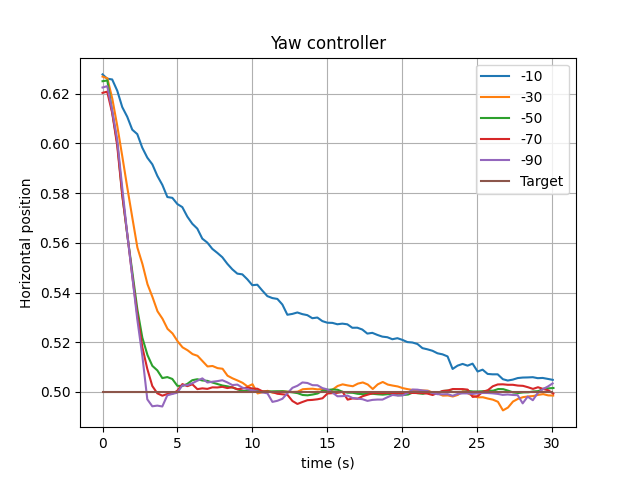
\includegraphics[width=.52\textwidth]{img/pid/yaw/yaw_pos_prop_i0_d0.png}
%   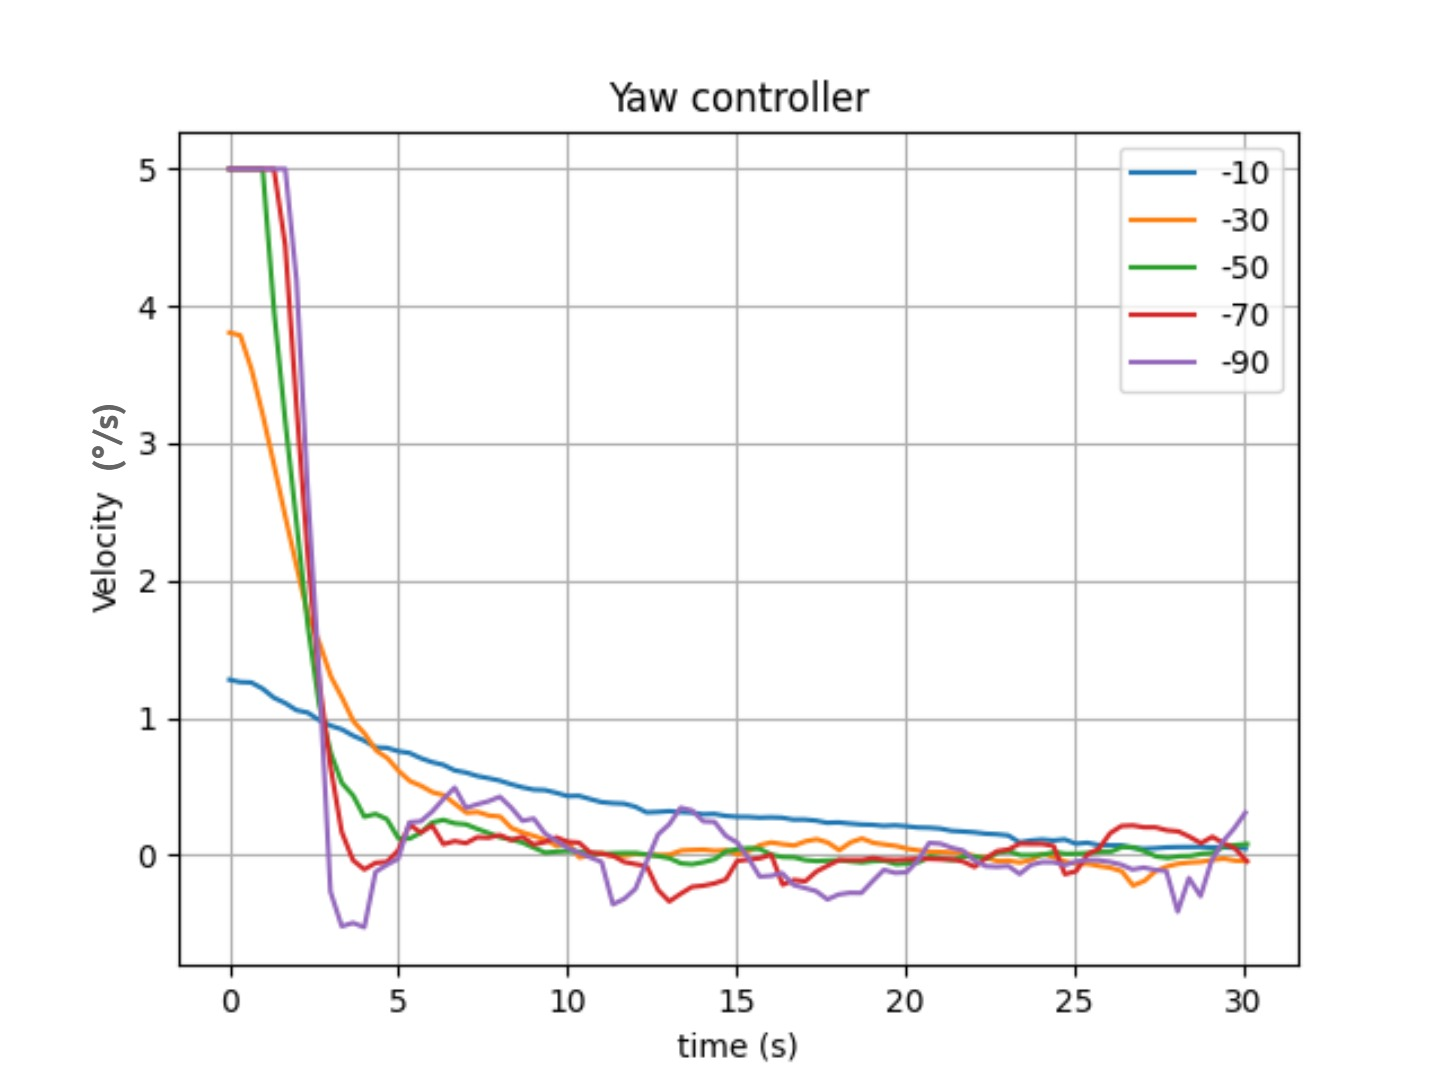
\includegraphics[width=.52\textwidth]{img/pid/yaw/yaw_vel_prop_i0_d0.jpg}}
%   \caption{Variation of (a) input position and (b) output velocity for different values of $K_{P}$ and $K_I=0$, $K_D=0$ while the yaw controller is engaged.}\label{fig:tune-yaw-prop}
% \end{figure}





\subsection{Forward controller}

After the yaw controller is tuned, it is time to move to the forward controller.
The process will be the same as for the yaw controller. Looking at the process gain in this case, it can be noted that a positive output in the controller creates a positive velocity in the forward direction, drawing the vehicle closer to the target person. The input variable is the height of the detected person in the camera field of view, normalized to the height of the field of view, which increases as the drone gets closer to the target. Therefore, a positive output velocity results in an increasing input to the controller, which means that the controller gain already has the correct sign.

The starting position for tuning the forward controller needs to present an offset from the reference position in the distance between the person and the vehicle (x-axis). To achieve this, the person model will be situated at the $x=500, y=0$ coordinates, with the vehicle remaining at the origin in the simulated world. The chosen starting position (closer than the reference point) will result in an initial negative velocity output to move the vehicle away from the person. Figure \ref{fig:tune-ref-pos-fwd} shows the starting position in the simulator.


\begin{figure}[H]
  \centering
  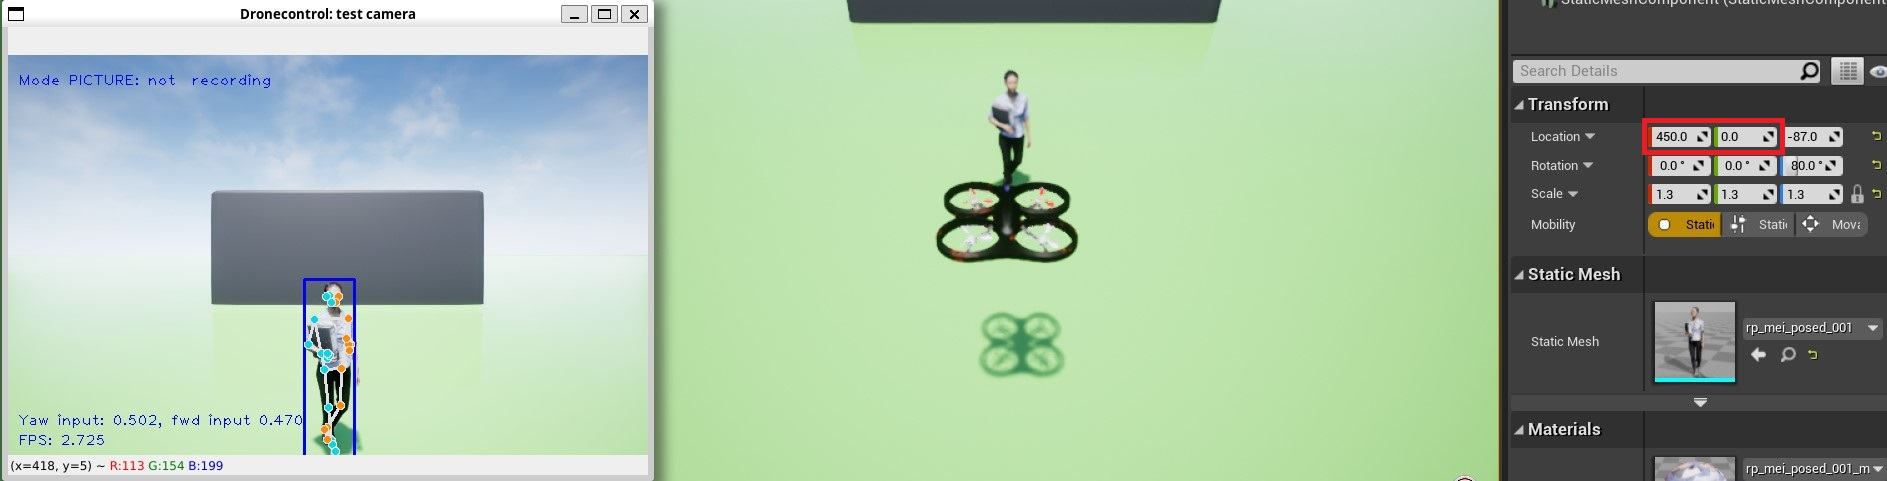
\includegraphics[width=\textwidth, keepaspectratio]{img/pid/tune-ref-pos-fwd.jpg}
  \caption{Starting position of the simulator for tuning the forward controller. The human model is situated 450 units forward and centred from the vehicle position.}\label{fig:tune-ref-pos-fwd}
\end{figure}



\subsection{PID tuning validation}
\label{subsec:pid-test-controller}

The final validation of the tuning obtained for the controllers will be performed using the \texttt{test-controller} tool described in Section \ref{subsec:pid-tools}. The goal is to check the step response of the controllers for different starting distances and validate their performance when engaged simultaneously. For the first test, the starting distances will vary along the y-axis, and for the second one, they will vary along the x-axis.

In the first test, the positions will vary along the y-axis, meaning that the figure will move from left to right in the field of view of the vehicle. The y-coordinates to be tested will range from -150 to 150 units in increments of 50, while the x-coordinate of the figure in the simulated world will remain fixed at $x=500$.

The results of the first run are shown in Figure \ref{fig:validate-yaw}. The y-coordinates tested range from -150 to 150 units in increments of 50, while the x-coordinate of the figure in the simulated world remains fixed at $x=500$. These changes in position mean that the figure moves from left to right in the field of view of the vehicle, following a line parallel to the lateral axis of the vehicle. To counteract this movement, both the yaw and forward controllers need to engage to reach the reference position.

The plots in Figure \ref{fig:validate-yaw} depict the changes in the normalized horizontal distance and normalized figure height detected by the person recognition algorithm during the time it takes for the vehicle to reach the target distance from the human figure for each tested start position. The target is considered reached when the error is less than 2\% and the output speed at the controller is less than 10\% of the maximum value. The full execution of the \texttt{test-controller} tool with varying lateral positions can be seen in the video found in the project's \href{https://l-gonz.github.io/tfg-giaa-dronecontrol/videos/test-yaw-controller}{page}\footnote{\url{https://l-gonz.github.io/tfg-giaa-dronecontrol/videos/test-yaw-controller}}.

\begin{figure}[H]
  \centering
  \makebox[\textwidth][c]{
  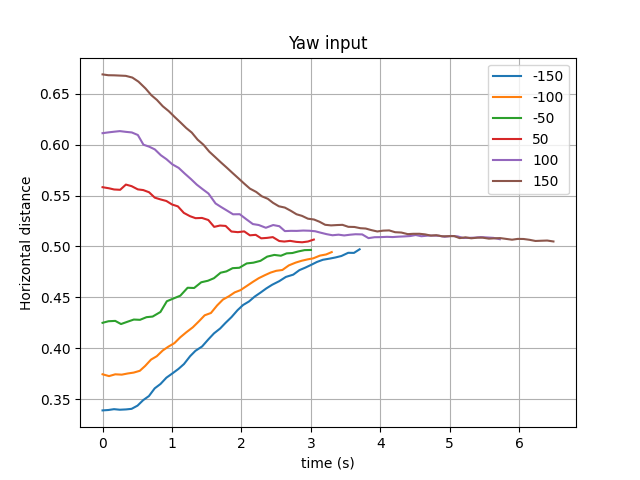
\includegraphics[width=.52\linewidth]{img/pid/validation_yaw.png}
  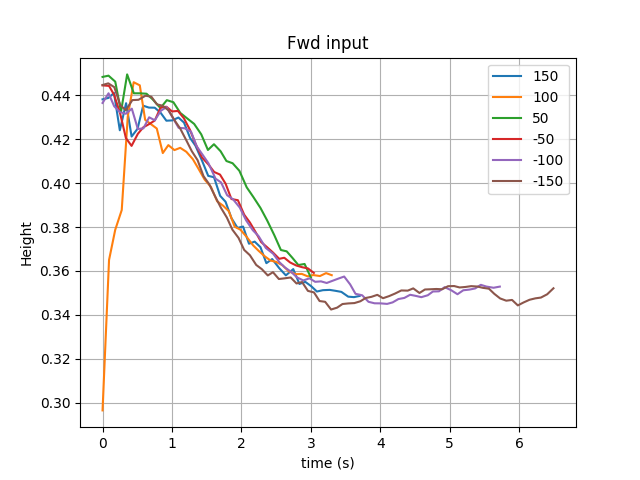
\includegraphics[width=.52\linewidth]{img/pid/validation_yaw_2.png}}
  \caption{Changes over time in detected horizontal position and height as input for the controllers with different starting positions in the y-axis.}
  \label{fig:validate-yaw}
\end{figure}

During execution, the yaw controller introduces a negative yaw velocity when the figure is on the left half of the camera's field of view and a positive yaw velocity when the figure is on the right half, aiming to achieve a target horizontal distance of 0.5 (centred in the camera image). On the other hand, the forward controller outputs a negative forward velocity to reduce the detected height of the figure from around 0.44 to the target value of 0.36.

Looking at Figure \ref{fig:validate-yaw}a, it can be observed that most of the time is spent initiating the movement towards the target. Once the vehicle starts moving, there is not much difference between the -50 and the -150 steps in the time it takes to reach the target position, with the former taking around 3 seconds and the latter taking approximately 3.6 seconds. 

In Figure \ref{fig:validate-yaw}b, the trajectories appear quite similar since the starting distance to the target is the same for all the cases. For each run, the controller guides the vehicle to move backwards, ensuring that the figure stays sufficiently far away, resulting in a decrease in the detected height. Additionally, a detection anomaly can be observed in Figure \ref{fig:validate-yaw}b. For the starting position at $y=100$ (yellow line), there is a brief initial period where the detected height is very small due to a detection error in the first frames processed by the computer vision algorithm. However, within half a second, the detection stabilizes, and the controller successfully guides the vehicle to the target position without significantly impacting the time taken or the final position. This demonstrates that the controllers are capable of recovering from detection errors without compromising the vehicle's movement.


\begin{figure}[H]
  \centering
  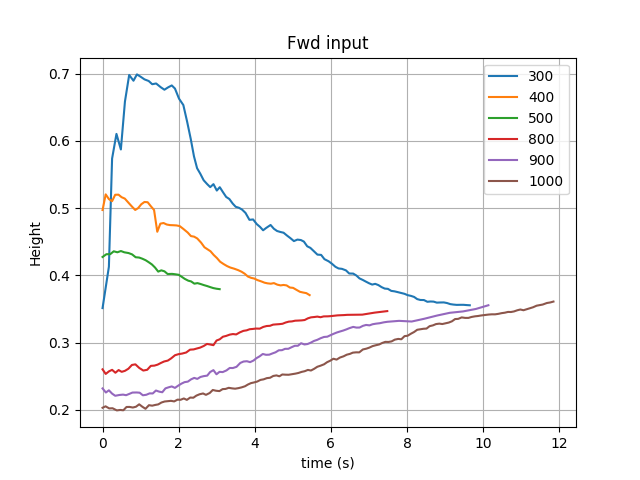
\includegraphics[width=.7\textwidth, keepaspectratio]{img/pid/validation_fwd.png}
  \caption{Changes over time in detected height as input for the forward controller with different starting positions in the x-axis.}
  \label{fig:validate-fwd}
\end{figure}


To further validate the performance of the forward controller, the \texttt{test-controller} tool can be used with varying positions along the x-axis. This means that the tests are conducted with the human figure at different distances along the longitudinal axis of the vehicle, closer and further away than the reference distance. Throughout the process, the figure is kept centred in the camera's field of view (y position remains 0). Therefore, in this scenario, the yaw controller does not need to be considered.

Figure \ref{fig:validate-fwd} illustrates the changes over time in the input to the forward controller for each starting position as the vehicle moves towards the target position. The graph highlights significant differences in how the controller responds to positions closer or further away from the target distance. When the person is very close to the vehicle, there are substantial differences in detected heights for minor changes in longitudinal distance, leading to the rapid movement of the vehicle away from its start position. Conversely, when the person is further away from the vehicle than the target, the same differences in distance are associated with minor differences in detected height. As a result, the controller determines a smaller velocity output compared to the cases when the person is closer to the vehicle. Consequently, it takes a longer time for the vehicle to reach the target position.

Notably, even when the person is so close to the vehicle that part of their figure falls outside the camera's field of view, the pose detection mechanism functions well enough to estimate the person's continued position outside the image. This can be seen on Figure \ref{fig:validate-fwd} for the case of $x=300$, where the detected height starts lower than it should be and gradually increases as the full person starts to fit in the camera's field of view.
\\ \\


\begin{figure}[H]
  \centering
  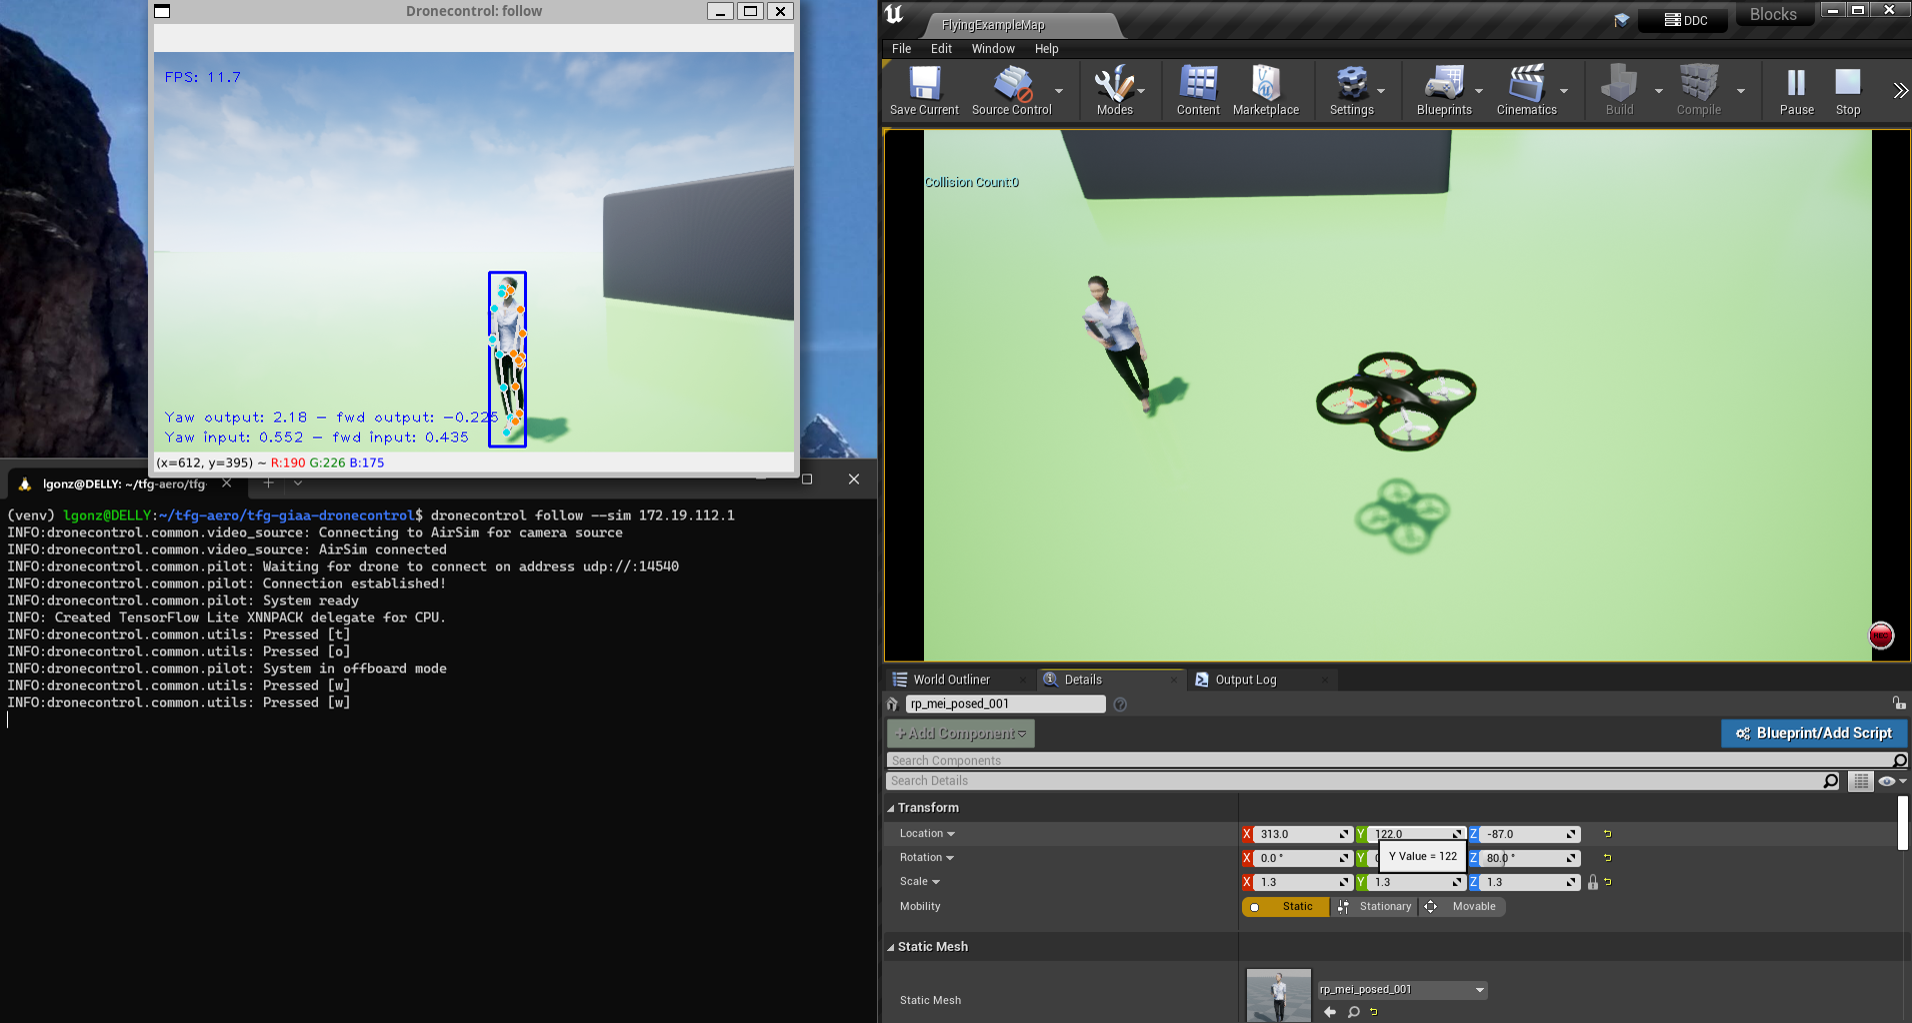
\includegraphics[width=\textwidth, keepaspectratio]{img/video-follow-sitl.png}
  \caption{Single frame from the video showing the movement of the drone in response to changes in the position of the tracked person.}
  \label{fig:airsim-test-follow}
\end{figure}

Overall, the results of the validation process indicate that the tuned controllers perform effectively, and accurately follow the person across different starting positions, even when detection errors occur. They successfully respond to variations in the person's distance and angle from the vehicle, allowing for accurate tracking and movement towards the target relative position.

The selected coefficients for the controllers can now be applied to the complete follow solution in order to assess the expected performance of the vehicle in real flights. To provide a visual demonstration, a video showcasing the drone's movement using these parameter values can be accessed \href{https://l-gonz.github.io/tfg-giaa-dronecontrol/videos/test-sitl-follow}{here}\footnote{\url{https://l-gonz.github.io/tfg-giaa-dronecontrol/videos/test-sitl-follow}}. Additionally, Figure \ref{fig:airsim-test-follow} displays a frame extracted from the video, giving a glimpse of the drone's behaviour during the follow operation.



